%!TEX encoding = utf8
%!TEX TS-program = xelatex
\documentclass[12pt, twoside]{book}
%\usepackage[T1]{fontenc}
% \usepackage[utf8]{inputenc}
\usepackage[spanish, english]{babel}
\usepackage[table,xcdraw]{xcolor}
%% FONTS: libertine+biolinum+stix
% \usepackage[mono=false]{libertine}
% \usepackage[notext]{stix}
%\usepackage{fontspec}
\usepackage{setspace}
\usepackage[hidelinks, linkcolor=USred]{hyperref}
\usepackage{longtable}
\usepackage{hhline}
\usepackage{booktabs}

%\usepackage{MinionPro}
%\usepackage{MnSymbol}
%\setmainfont{Minion Pro} 
%\usepackage[textlf,mathlf]{MinionPro}
%\usepackage[minion,vvarbb,cmbraces,cmintegrals]{newtxmath}
%\defaultfontfeatures{Mapping=tex-text}
%\setmainfont
%[BoldFont=MinionPro-Bold.otf,
% ItalicFont=MinionPro-It.otf,
% BoldItalicFont=MinionPro-BoldIt.otf]
% {MinionPro-Regular.otf}

 
%\newfontfamily\headingfont[ItalicFont=MinionPro-BoldIt.otf]{MinionPro-Bold.otf}
%%%

\title{Machine Learning in Parkinson's Disease Diagnosis}
\author{Max Wang}
\date{\today}

% ======================
% = Páginas de títulos =
% ======================
\makeatletter
\edef\maintitle{\@title}
\renewcommand\maketitle{%
    
  \begin{titlepage}
  \parindent=0pt
  \begin{flushleft}
  \vspace*{1.5mm}
  \setlength\baselineskip{0pt}
  \setlength\parskip{0mm}
  
  \begin{center}
%   \sffamily College Of Engineering\\[4pt] \hspace{-10pt}\& Computer Science
  \end{center}
\centering
\includegraphics[width=0.3\linewidth]{anulogo.jpg}
\vspace{-10pt}
\begin{center}
   \sffamily Australian National University
  \end{center}
  \end{flushleft}
  \vspace{1cm}
  \bgroup
  \huge \bfseries
  \begin{center}
  {Machine Learning in \\Parkinson's Disease Diagnosis}
  \end{center}
  \egroup
  \vspace*{.5cm}
  \begin{center}
  {\large{Bachelor's Thesis}}\\
  {\LARGE{\@author}}
  \end{center}
  \vspace*{5cm}
  \begin{flushright}\sffamily{Supervised by: \\[-4pt]
Dr Deborah Apthorp\\[-4pt]
Dr Hanna Suominen }
  \end{flushright}
   \end{titlepage}
   \pagestyle{tfg}
   \renewcommand{\chaptermark}[1]{\markright{\thechapter.\space ##1}}
   \renewcommand{\sectionmark}[1]{}
   \renewcommand{\subsectionmark}[1]{}
  }
\makeatother

% ======================================
% = Color de la Universidad de Sevilla =
% ======================================
\usepackage{tikz}
\definecolor{USred}{cmyk}{0,1.00,0.65,0.34}

\usepackage{caption}
\usepackage[font={},figurename=Fig.,labelfont={it, color=USred,bf}]{caption}
% =========
% = Otros =
% =========
\usepackage[]{tabularx}
\usepackage[]{enumitem}
\setlist{noitemsep}

% ==========================
% = Matemáticas y teoremas =
% ==========================
\usepackage[]{amsmath}
\usepackage[]{amsthm}
\usepackage[]{mathtools}
\usepackage[]{bm}
\usepackage[]{thmtools}
\usepackage{amssymb}
%\usepackage{bbold} 
\usepackage[quiet]{mathspec}
\defaultfontfeatures{Mapping=tex-text}
\setmathsfont(Digits)[Uppercase=Regular,Lowercase=Regular]{MinionPro-Regular.otf}
\setmathsfont(Latin)[Uppercase=Italic,Lowercase=Italic]{MinionPro-It.otf}
\setmathsfont(Greek)[Uppercase=Regular,Lowercase=Italic]{MinionPro-It.otf}
\setmathrm{Minion Pro} 
\setmainfont[Ligatures         = {Common,TeX}, 
SmallCapsFeatures = {Letters     = SmallCaps,%
	Numbers     = Lowercase,
	Kerning     = Uppercase,
	LetterSpace = 5},
    BoldFont=MinionPro-Bold.otf,
	ItalicFont=MinionPro-It.otf,
	BoldItalicFont=MinionPro-BoldIt.otf]
	{MinionPro-Regular.otf}

%\defaultfontfeatures{Mapping=tex-text}
%\setmainfont
%[BoldFont=MinionPro-Bold.otf,
% ItalicFont=MinionPro-It.otf,
% BoldItalicFont=MinionPro-BoldIt.otf]
% {MinionPro-Regular.otf}


%\usepackage{unicode-math} % try sans-style=upright
%\usepackage{xltxtra}

\newcommand{\marcador}{\vrule height 10pt depth 2pt width 2pt \hskip .5em\relax}
\newcommand{\cabeceraespecial}{%
    \color{USred}%
    \normalfont\bfseries\itshape}
\declaretheoremstyle[
    spaceabove=\bigskipamount,
    spacebelow=\smallskipamount,
    headfont=\cabeceraespecial\marcador\itshape,
    notefont=\cabeceraespecial\itshape,
    notebraces={(}{)},
    bodyfont=\normalfont,
    postheadspace=1em,
    numberwithin=chapter,
    headindent=0pt,
    headpunct={.}
    ]{importante}
\declaretheoremstyle[
    spaceabove=\medskipamount,
    spacebelow=\medskipamount,
    headfont=\normalfont\itshape\color{USred}\centering,
    notefont=\normalfont\centering,
    notebraces={(}{)},
    bodyfont=\normalfont\centering,
    postheadspace=1em,
    numberwithin=chapter,
    headindent=0pt,
    headpunct={.}
    ]{normal}
\declaretheoremstyle[
    spaceabove=\medskipamount,
    spacebelow=\medskipamount,
    headfont=\normalfont\itshape\color{USred},
    notefont=\normalfont,
    notebraces={(}{)},
    bodyfont=\normalfont,
    postheadspace=1em,
    headindent=0pt,
    headpunct={.},
    numbered=no,
    qed=\color{USred}\marcador
    ]{demostracion}

% Los nombres de los enunciados. Añade los que necesites.
\declaretheorem[name=Note, style=importante]{note}
\declaretheorem[name=Highlight, style=importante]{highlight}
\declaretheorem[name=Corollary style=normal]{corollary}
\declaretheorem[name=Propositon, style=normal]{proposition}
\declaretheorem[name=Lemma, style=normal]{lemma}

\declaretheorem[name=Fig, style=normal]{fig}

\declaretheorem[name=Theorem, style=importante]{theorem}

\let\proof=\undefined
\declaretheorem[name=Demonstration, style=demostracion]{proof}

\newcommand*{\specialcellbold}[2][b]{%
  \bfseries\sffamily\color{USred}
  \begin{tabular}[#1]{@{}c@{}}#2\end{tabular}%
}

\def\specialcell#1{$\vtop{\halign{\hfil##\hfil\strut\cr#1\cr}}$} 

\def\specialcellright#1{$\vtop{\halign{\hfil##\hfil\strut\cr#1\cr}}$} 

\renewcommand\emph[1]{\textit{\color{USred}{#1}}}
% ============================
% = Composición de la página =
% ============================
\usepackage[
	a4paper,
    margin=1.2in
%     textwidth=80ex,
]{geometry}

\linespread{1.3}
\parskip=14pt plus 1pt minus .5pt
\frenchspacing
% \raggedright


% ==============================
% = Composición de los títulos =
% ==============================

\usepackage[explicit]{titlesec}

\newcommand{\hsp}{\hspace{20pt}}
\titleformat{\chapter}[hang]
    {\Huge\sffamily\bfseries}
    {\textcolor{USred}{\thechapter}\hsp\textcolor{USred}{\vrule width 2pt}\hsp}{0pt}
    {#1}
\titleformat{\section}
  {\normalfont\Large\sffamily\bfseries}{\textcolor{USred}{\thesection}\space\space}
  {1ex}
  {#1}

\titleformat{\subsection}
  {\normalfont\large\sffamily}{\textcolor{USred}{\thesubsection}\space\space}
  {1ex}
  {#1}
  
\titleformat{\subsubsection}
  {}
  {}
  {0ex}
  {\textcolor{USred}{\sffamily{\textbf{#1}}}}
  
  
\renewcommand\thefootnote{\textcolor{USred}{\arabic{footnote}}}

 \titlespacing{\section}{0ex}{1.2ex plus .1ex minus .5ex}{-0.4ex}
  
 \titlespacing{\subsubsection}{0ex}{0.6ex plus .1ex minus .5ex}{-0.7ex}

 \titlespacing{\subsection}{0ex}{1ex plus .1ex minus .5ex}{-0.6ex}

% =======================
% = Cabeceras de página =
% =======================
\usepackage[]{fancyhdr}
\usepackage[]{emptypage}
\fancypagestyle{plain}{%
    \fancyhf{}%
    \renewcommand{\headrulewidth}{0pt}
    \renewcommand{\footrulewidth}{0pt}
}
\fancypagestyle{tfg}{%
    \fancyhf{}%
    \renewcommand{\headrulewidth}{0pt}
    \renewcommand{\footrulewidth}{0pt}
    \fancyhead[LE]{{\normalsize\color{USred}\bfseries\thepage}\quad
                    \scriptsize{\MakeUppercase{\maintitle}}}
    \fancyhead[RO]{\scriptsize{\MakeUppercase{\rightmark}}%
                    \quad{\normalsize\bfseries\color{USred}\thepage}}%
}
                    
% =============================
% = El documento empieza aquí =
% =============================
\begin{document}

\maketitle
\begin{spacing}{-0.2}
\tableofcontents
\end{spacing}


\mainmatter


\chapter*{Abstract}
\addcontentsline{toc}{chapter}{Abstract}
\markright{Abstract}
Parkinson's disease (PD) is a degenerative neurological disorder, affecting around 1\% of the population by the age of 70. There is currently no objective test for PD and studies suggest expert misdiagnosis rates of up to 34\%. Hence, there is interest in investigating if machine learning can provide a more reliable and objective diagnosis.

Current machine learning literature test a model's ability to differentiate between already diagnosed PD and control subjects. This setup does not mirror real-life diagnosis as the primary difficulty neurologists face is excluding disorders with similar symptoms and individuals exhibiting minimal symptoms. Most studies are also based on small (<50) datasets which suffer from a tendency to bias and overfitting due to  Freedman's paradox. A large dataset of individuals pre-diagnosis to confirmed diagnosis would be optimally be used to assess machine learning in PD.  

This thesis investigates the applicability of machine learning in PD diagnosis by testing a model's ability to diagnose PD using symptoms unobservable by a neurologist. Current literature is replicated on the much larger 6,000 participant mPower dataset, consisting of crowdsourced recordings from smartphone sensors. Results showed that the simple models used in current literature are insufficient for a reliable diagnosis using the large and noisy mPower data. More powerful and robust models were developed by consolidating recent ideas EEG and non-linear signal processing, deep learning and computer vision, resulting in improvement from XX\% to YY\% accuracy.
 

%This thesis focuses on answering the question: ``what can machine learning offer the field of PD diagnosis?''. We approached this by investigating the ability for machine learning to differentiate PD and non-PD participants based on symptoms neurologists could not identify. 

%We propose a number of techniques to handle the noise in the mPower data and show that the simpler machine learning models used in past works are insufficient to handle 

Results suggest that machine learning can offer a valuable source of information for experts as these models quantify symptoms differently from experts. --more discussion here--

\chapter*{Introduction}
\addcontentsline{toc}{chapter}{Introduction}
\markright{Introduction}
This thesis has been written for all audiences, however a background in machine learning may be useful to understand and follow some assumptions in the methodology. The work spans multiple disciplines and I have opted to summarise these fields concisely and provide references to seminal or well-written papers in the area for the reader interested in a more in-depth understanding. These papers will also provide the mathematical formulation of the signal processing and machine learning models which have been abstracted in favour for the intuition behind them.

Throughout the thesis I have used highlights and footnotes to improve flow and reading. Highlights convey or re-iterate important information for those skim-reading and footnotes\footnote{\emph{Footnotes} provide contextual background information} provides contextual background information.

\vspace{5pt}
\begin{figure}[h]
\cabeceraespecial\marcador\itshape Highlight.\hspace{12pt} 
\normalfont \color{black} Highlights re-iterate crucial information.
\end{figure}
\vspace{-2pt}

The thesis is organised as follows:

Chapter \ref{bgchapter} summarises Parkinson's Disease and relevant prior work in the field of feature extraction and machine learning. The remainder of the thesis is written with the assumption that the reader understands this background, enabling it to be very concise. 

Chapter \ref{ourwork} begins with a literature review of relevant works in PD machine learning. 

Major contributions are...

%Prcessing power was a significant limitation. All processing was done on a roasted potato.

\chapter{Background}
\label{bgchapter}
\textit{Parkinson's disease} (PD) is a major health problem, affecting around 1\% of the population by age 70 \cite{savittdiagnosis1}. PD is a degenerative neurological disorder characterised by a regression of movement, speech and memory. There is currently no objective test for PD and diagnosis is especially difficult in its early stages as symptoms have not fully manifested \cite{brooksdiagnosis25}. Studies suggest that motor symptoms only manifest once 20-40\% of dopamine\footnote{
\emph{Dopamine} is a neurotransmitter that aids communications between neurons. As PD targets dopamine producing neurons, this leads to a decline in functionality of the Basal Ganglia which is associated with motor and cognitive control.  } producing cells have deteriorated~\cite{bernheimer1973brain}. The exact underlying causes of Parkinson's disease are still unknown~\cite{savittdiagnosis1}.


\begin{table}[h]
\centering

\caption{Symptoms of Parkinson's disease~\cite{savittdiagnosis1}. Although commonly associated with tremor, only around 70\% of patients experience resting tremor~\cite{pdtremorpercent2}.}

\begin{tabular}{c c c}
\toprule
{\specialcellbold{Movement}} &
{\specialcellbold{Voice}} &
{\specialcellbold{Non-motor}}\\
\midrule
\specialcell{Resting Tremor\\[4pt]
Rigidity\\[4pt]
Bradykinesia\\
(Slow Movement)\\[4pt]
Dyskinesia\\
(Involuntary Movement)\\[4pt]
Akinesia \\
(Freezing of Gait)}
&
\specialcell{
Reduced Volume\\[4pt]
Monotonous Speech\\[4pt]
Imprecise Articulation\\[4pt]
Slurred Speech\\[4pt]
Hesitant Speech
}
&
\specialcell{
Hallucinations\\[4pt]
Reduced Cognitive Ability\\[4pt]
Sleep Disorders\\[4pt]
Mood Disorders\\[4pt]
Vision Problems\\[4pt]
Physical Changes\\
}\\
\bottomrule
\end{tabular}
\end{table}


Current treatments provide temporary relief from symptoms and have been shown to slow disease progression \cite{slowprog1, slowprog2, slowprog3} . Thus, an accurate early diagnosis is crucial to ensuring a higher quality of life later in life. 

PD is currently diagnosed with a subjective test by a neurologist~\cite{tolosadiagnosis26}. This test generally involves qualifying visible symptoms such as tremor and dysphonia, and assessing the patient's response to Levodopa\footnote{\emph{Levodopa} is the most common medication for Parkinson's disease. It is converted to dopamine --- replenishing the patient's deficit --- however it often results in side-effects such as depression and fatigue.}. As visible symptoms do not manifest until later stages, an early stage diagnosis is rare. There has been research in qualifying minor changes in speech \cite{hazan2012,earlyvowel}, sleep, olfactory and gastrointestinal behaviours \cite{earlynonmotor, genemarkers} as early markers of the disease. 


The primary difficulty in diagnosis is differentiating from other Parkinsonism\footnote{\emph{Parkinsonism} movement disorders are those with similar symptoms to PD.} disorders such as Multiple System Atrophy, Supranuclear Palsy and Essential Tremor~\cite{parkinsonismdifferential1}. Confirmation of diagnosis is generally only possible with an autopsy. As there is no definitive test and symptoms resemble other neurological disorders, misdiagnosis rates are high. Studies suggest a misdiagnosis rate is high, ranging from 9--34\% depending on methodology~\cite{tolosadiagnosis26, brooksdiagnosis25, jankovic2000evolution}. 


\begin{highlight}[Diagnosis]
PD is diagnosed subjectively by a neurologist. As many disorders have similar symptoms, the misdiagnosis rate is high --- up to 34\%.
\end{highlight}

As there is no consensus for PD diagnosis, the search for a more objective measure for PD is a hot topic in the research community. This ranges from more standardised diagnosis criteria such as the UK Parkinson's Disease Society Brain Bank criteria \cite{tolosadiagnosis26,brainbank,hughesdiagnosis100} to discovering more quantifiable biomarkers such as gene expression \cite{genemarkers, genome} and proteins in bodily fluids \cite{biomarkerfluid}. Although the discovery of objective biomarkers shows promise, it is likely that cost would be prohibitive for most early stage patients.

\section{Machine Learning in Parkinson's Disease}
Machine Learning can be broadly defined as a suite of computational techniques that address the challenge of making sense of the ever increasing volume and complexity of data generated in, for example, modern information dense healthcare system. It will be examined in greater depth in section~\ref{machinelearning}.

Machine learning presents an objective and low cost solution to diagnosing PD. There has been a large body of work in the field however the applicability all current work is limited due to the cost and difficulties associated with gathering a sizeable dataset. A majority of datasets used in literature consist of fewer than 40 subjects. Reported results are therefore prone to biases in the dataset, Freedman's paradox\footnote{\emph{Freedman's paradox} describes a common issue in model fitting where variables with no predictive power appear important. It is especially prevalent when the number of features exceeds the number of data points.}~\cite{freedmanparadox} and overfitting on cross validation~\cite{overfittingcv}. Thus, it is difficult to empirically compare results of different papers.

%. An example of bias would be the PD subjects coincidentally having naturally deeper voices than the control subjects. Thus, comparisons of results are difficult. 

\begin{highlight}
It is difficult to compare and evaluate work in PD machine learning due to variation in data and small dataset sizes.
\end{highlight}

There has been preliminary investigation in the applicability of machine learning in differentiating PD and other Parkinsonism disorders with promising results~\cite{esser2011assessment, PDessentialtremordifferentiation}. However a majority of literature in the field uses machine learning to differentiate between PD and control subjects. This artificial setup simplifies the complexities involved in a neurologist's diagnosis for PD. As patients have already been diagnosed with PD, they likely exhibit noticable symptoms. Neurologists must perform diagnosis in early stages when symptoms are not evident and must consider the possibility of any number of causes for the symptoms. Current methods in machine learning only show its ability to detect the symptoms associated with PD and are difficult to relate to real world diagnosis. 

\begin{highlight}
Current research tasks machine learning to differentiate between PD and control subjects. This is a much simpler problem than what is faced by neurologists who have to rule out a number of other possibilities for symptoms.
\end{highlight}

To precisely compare the effectiveness of machine learning to neurologist diagnosis, a large \emph{longitudinal dataset} following subjects pre-diagnosis to a confirmed diagnosis would be required. Such a dataset would be very costly and logistically difficult to collect. To advocate the collection of such a dataset, some evidence of machine learning's applicability to PD diagnosis will be required. This thesis will investigate methods of assessing machine learning's applicability to Parkinson's disease without such a dataset.  

Another proposed application for machine learning for PD is telemonitoring~\cite{splittledysphonia2009, sptsanastelemonitor2010}. A patient's progression of PD is monitored with a scale, the most common being the MDS-UPDRS~\cite{updrs} which quantifies the extent of 27 motor and non-motor symptoms on an integer scale between 0-4, with 0 representing no evidence of symptoms and 4 indicative of severe symptoms. It is recommended that PD patients visit a specialist every 4-6 months to track progression --- this is costly and inconvenient. Machine learning offers the opportunity for patients to track their progress at home with their smartphone or other wearables~\cite{cancela2016monitoring}. Monitoring is a viable avenue for machine learning given current datasets, however will not be explored in this thesis as the primary focus is diagnosis.

\begin{highlight}[UPDRS]
The MDS-UPDRS~\cite{updrs} scale quantifies the extent of 44 motor and non-motor symptoms on a scale of 0-4. It is currently assessed by a neurologist.
\end{highlight}

The machine learning process for classification can generally be divided into two steps:
\begin{enumerate}[noitemsep, topsep=-10pt]
\item \emph{Feature extraction --- } From the raw input data from devices such as Accelerometers or microphones, features such as pitch and amplitude are quantified. 

\item \emph{Feature and Model selection -} A machine learning model is selected and its hyperparameters tweaked to to best suit the problem.  The set of features used by the model is often reduced using feature selection~\cite{featureselection} and dimensionality reduction~\cite{pca, ica} due to the curse of dimensionality\footnote{The \emph{curse of dimensionality} states that  exponentially more training data is often required for each additional feature to ensure a complete and reliable model.}~\cite{curseofdimensionality}. 
\end{enumerate}

\section{Feature Extraction and Signal Processing}
Feature extraction is the process of converting raw input data (\emph{signals}) into meaningful numerical values\footnote{This is not required for all sensors data (e.g cameras and MRIs) however is generally required for any time-series sensor.}. For example, with sensors such as microphones, features such as pitch and volume may be extracted. Features should relate to the machine learning task as most machine learning models perform poorly as more unrelated features are added. Understanding raw input data and extracting useful features is a primary component in the field of \textit{digital signal processing}. 

Movement related problems are the primary manifestation of symptoms considered by a neurologist when diagnosing PD. Human vision is very advanced and captures and processes a great deal of information about the world around us. Through years of experience, we have learned the general behaviour of human movement, hence minor tremor and slight deviations from normal gait are very noticeable. However, our ability to differentiate between forms of irregular gait is more limited~\cite{parkinsonismdifferential1}. Although sensors such as IMUs can only a capture a fraction of the information of human eyes, it is possible that they are better at detecting the differences between forms of irregular gait~\cite{parkinsonismdifferential2}.

\begin{highlight}
Our senses are good at detecting deviations from normal gait/speech, but are less proficient at detecting differences between types of abnormal gait/speech. 
\end{highlight}

Although speech is only a single component of the 44 component UPDRS~\cite{updrs} scale, it has received a great deal of attention in machine learning. There is evidence that speech is one of the earliest indicators of PD \cite{earlyvowel} and there already exists a large body of work in the field of speech feature extraction~\cite{ostextbook}. Furthermore, microphones are able to capture a similar level of information as human ears --- there is much less information loss compared to sensors used to measure movement\footnote{Excepting motion capture, which we will cover in section \ref{movementfeatures}.}. 


Table \ref{pdsensors} summarises prior work in feature extraction related to PD. As most datasets consist of data from a single sensor, machine learning focuses on quantifying a single symptom of Parkinson's disease based on that sensor. Literature can be classified as diagnosing PD with movement or voice features and currently more research focuses on movement~\cite{review2013,review2015}.


\begin{table}[h]
\caption{Prior work in the field of PD diagnosis. The signal processing of sensor data is often more important that the machine learning model.}

\label{pdsensors}
\centering
\begin{tabular}[t]{c c c}
\toprule
{\specialcellbold{Movement}} &
{\specialcellbold{Voice}} &
{\specialcellbold{Non-motor}}\\
\midrule

\begin{tabular}[t]{@{}l@{}}Resting Tremor\\ 
\hsp IMUs\protect\footnotemark~\cite{duval2004detection,salarian2007tremor,palmerini2011tremor}\\
\hsp Smartphones~\cite{arora2014high,smartphonemjfoxB,smartphonemjfoxlion}\\[4pt]
Postural Sway\\ 
\hsp Force Plates~\cite{rocchi2006identification}\\
\hsp IMUs~\cite{imupostural,palmerini2011tremor}\\[4pt]
Gait\\ 
\hsp Force Walkways~\cite{begg2006neural,roiz2010gait,khorasani2014hmm}\\
\hsp Video~\cite{roiz2010gait}\\
\hsp Multiple IMUs~\cite{barth2011biometric,renaudin2012step,sijobert2015implementation}\\[4pt]
Handwriting~\cite{drotar2015handwriting,drawing}\\[4pt]
Motion Capture~\cite{das2011quantitative}\\[4pt]
Tapping~\cite{tapping,zhan2016high}
\end{tabular}
& 
 
\begin{tabular}[t]{@{}l@{}}Words and\\sentences\\\cite{hazan2012,compareis15pd,orozco2015voiced}\\[4pt]
Sustained vowel\\phonation\\
\cite{splittledysphonia2009, cnockaert2008,sakar2012}\end{tabular}
&
\begin{tabular}[t]{@{}l@{}}Demographics\\[4pt]
UPDRS Patient\\Questionnaire~\cite{nonmotordiagnosis,ppmigood}\\[4pt]
Physical Changes\\
\hsp Gene Expression~\cite{genemarkers,geneprediction}\\
\hsp MRI~\cite{mri1,mri2, mri3}\\
\hsp EEG~\cite{eegnonlinearpd, eegslowingpd}\\
\hsp Olfactory~\cite{nonmotordiagnosis}\\
\hsp REM sleep~\cite{nonmotordiagnosis, ppmigood}\\
\hsp Cerebrospinal Fluids~\cite{ppmigood}\\
\hsp Gastrointestinal~\cite{gastrointestinal}\end{tabular}
\\
\bottomrule
\end{tabular}
\end{table}

\addtocounter{footnote}{-1}
\footnotetext{Inertial Measurement Units (\emph{IMUs}) are electronic devices which measure both acceleration (x,y,z) and direction (pitch, roll, yaw) over time. This is generally done with an accelerometer and gyroscope.}

There is evidence that PD is heterogeneous and symptoms are present in distinct subsets \cite{subtypes, thenganatt2014parkinsonsubtypes}, however the underlying reasons not well understood. Studies have reported speech dysfunction present in  74-94\% of patients with PD \cite{ramig2008speech, sppercentage2,sppercentage3,sppercentage1}. Tremor is reported in 70\% of patients~\cite{pdtremorpercent1} and Akinesia in 80\%~\cite{pdtremorpercent2}. As neurologist diagnosis relies on judgement from observation, there is the possibility that some of these symptoms exhibit in a form imperceptible to a neurologist but detectable by a high resolution sensor. 

\begin{highlight}
It is possible that some subtypes of PD exhibit symptoms imperceptible to a neurologist but detectable by a high resolution sensor. 
\end{highlight}

Unless there is evidence that `\textit{micro-symptoms}' are present in all people with PD, feature extraction in each of these areas are equally as important. Section \ref{speechbio} explores some of the biological causes of these symptoms and we will investigate the existence of  micro-symptoms in section X.X


Section \ref{featuresummary} summarises all features that will be used in this paper. Feature extraction is not a simple task and information about the signal is almost always lost in the process. More recently, biologically inspired neural networks have been proposed to bypass the feature extraction step and extract information from raw representations of data. These will be covered in section \ref{neuralnetworkintro} and their applicability investigated in section X.X.

\subsection{General Signal Processing}
This thesis will focus on signal processing for time-series sensor data. The signal can be represented as an array with time on one axis and the sensor measurements on the other. The \textit{frequency} of a signal refers to the rate at which measurements are made (in measurements/second). For example, an average microphone would record the value of a sound wave at around 44.1kHz whereas an IMU would record six values for acceleration and rotation in the \textit{x, y} and \textit{z} direction at a frequency of 100Hz (phones) to 4000Hz. \textit{Noise} refers to deviations between the measured and true values, generally introduced by low quality recording equipment. This section outlines simple signal processing techniques which can be applied in most domains.


\emph{Moments} are basic statistical descriptors of a signal, with the first three moments representing mean, variance, skewness. Typically up to five moments are used in the signal processing of biological signals. For waveform signals such as voice, mean is generally uninformative and variance corresponds to volume whereas with accelerometer data the mean represents the average velocity of acceleration.  The zero or mean \emph{crossing rate} is a measure of how rapidly the signal oscillates around a certain value.

\emph{Entropy} describes the amount of information in a piece of data if it were modelled by a Bernoulli scheme. In the context of signal processing, it is a simple measure of the complexity of a signal. When there are two dimensions of data (e.g, $x$ and $y$ of an accelerometer) \emph{mutual information} and \emph{cross correlation} can be applied. Mutual information is a measure of the amount of information obtained of one signal when observing the other and cross-correlation is a measure of the similarity of the two signals. For continuous time signals these measures are approximate by binning the values, with a recommended $\sqrt{\frac{len}{5}}$ bins~\cite{entropymeasures}.

The \emph{Fourier} transform is one of the most fundamental tools in signal processing, decomposing a time-series signal into the magnitudes of frequencies that compose it. Given an accelerometer signal, the Fourier transform can be used to determine the amount of tremor in each frequency band - for example, PD tremor is exhibited as an increase in tremor in the 3.5-7Hz bands~\cite{duval2004detection}. The \textit{short time}\footnote{\emph{Short time} signal processing involves analysing short `windows' of the data to understand how it evolves over time. This provides more information but increases the complexity of analysis.} \textit{Fourier transform} (STFT) is often used when modelling evolving signals such as those generated during speech and walking.


% \ref{spectrogram}


\subsection{Voice}
PD diagnosis with vocal features is a promising option for diagnosis with machine learning as microphones are readily available and capture a comparable level of information to ears. Little~et~al.~(2009)~\cite{splittledysphonia2009} shows that audio from a phone is of sufficient quality to perform diagnosis with reasonable accuracy. This gives rise to the possibility of self diagnosis with a smartphone. However current feature extraction algorithms are sensitive to noise so robustness must be improved or bad recordings detected and filtered.


\subsubsection{Biological Background}
\label{speechbio}
Speech production consists of two components: the vocal folds and vocal tract. 

The vocal folds are housed in the larynx and consists of a flap called the \emph{glottis} which can be opened and closed. During speech production (phonation), air is expelled from the lungs builds pressure below the glottis. The imbalance of pressure below and above the glottis causes it to oscillate, producing sound. Muscles in the vocal folds enable adjustment the frequencies of sound produced within a certain range. The lowest of these frequencies --- the \textit{fundamental frequency}, \emph{$f_0$} --- correlates to duration of one oscillation and is denoted as the \textit{glottal cycle} or \textit{pitch period}. The higher frequencies are referred to as the \textit{harmonics} or \textit{overtones}. Physical characteristics such as age and especially gender affect the size of the vocal folds and range of sounds producible. 

The vocal tract comprises the components between the larynx and lips such as the mouth and nose. These components act as a resonator, `shaping' the sound by amplifying and attenuating certain frequencies produced by the vocal folds. The vocal folds and tract can be viewed as a \emph{source-filter model}, where the vocal folds (source) generates the sound (signal) which is shaped by the vocal tract (filter). 


Traditionally, the source-filter relationship of the vocal tract was assumed to be \textit{linear}\footnote{Mathematically, a \emph{linear function} $f$ satisfies $f(a+b) = f(a) + f(b)$ and $f(ab) = af(b)$.} and \textit{time invariant}\footnote{\emph{Time invariant} filters produce the same result for the same data independent of time or position.}. This assumption greatly simplifies the the analysis of speech and grants the use of a rich set of tools in the well-understood field of linear, time invariant systems theory. However, recent works in analysing speech provide strong evidence that these linear assumptions do not hold for most speech signals~\cite{nonlineardisorder, little2007biomechanically,titze2008nonlinear}. Non-linear signal analysis is still an experimental field and most algorithms estimate the true properties of underlying phenomena . Even determining the fundamental frequency from sustained vowel phonation is an inexact science as evident in Tsanas~et~al.~(2014)~\cite{f0estimation}.


PD vocal symptoms can be broadly classified as dysphonia~\cite{spworkshoptitze} --- impairment in the production of sounds and dysarthria~\cite{rosen2006parametric} --- difficulties in the articulation of speech. Dysphonia arises from problems in the vocal folds and dysarthria the vocal tract. 

\emph{Dysphonia} is often described as a `breathy' or `hoarse' voice. As fine motor control is diminished in people with PD, they exhibit incomplete vocal fold closure. Turbulent airflow causes each glottal cycle to vary more than a healthy speaker. However, similar phenomenon occurs when the vocal cords are damaged or irritated by causes such as colds. It is unknown whether differentiation between neurologically and physically cause dysphonia is possible.  

\emph{Dysarthria} arises from the loss of both motor and cognitive control. People with dysarthria experience hesitant speech as a result of slower cognition and slurred or imprecise articulation from the loss of fine motor control in the vocal tract. It is generally more difficult to to quantify as signal processing must be done in the short time domain. 


\subsubsection{Speech Signal Processing}
Parkinson's disease diagnosis with speech exists as two distinct subfields: quantifying dysarthria in spoken sentences and quantifying dysphonia with sustained vowels (e.g, `aaaaah...'). To obtain a clinical level diagnosis, both dysphonia and dysarthria related features will likely have to be considered.


\begin{figure}[h]
	\label{spectrogram}
	\centering\centerline{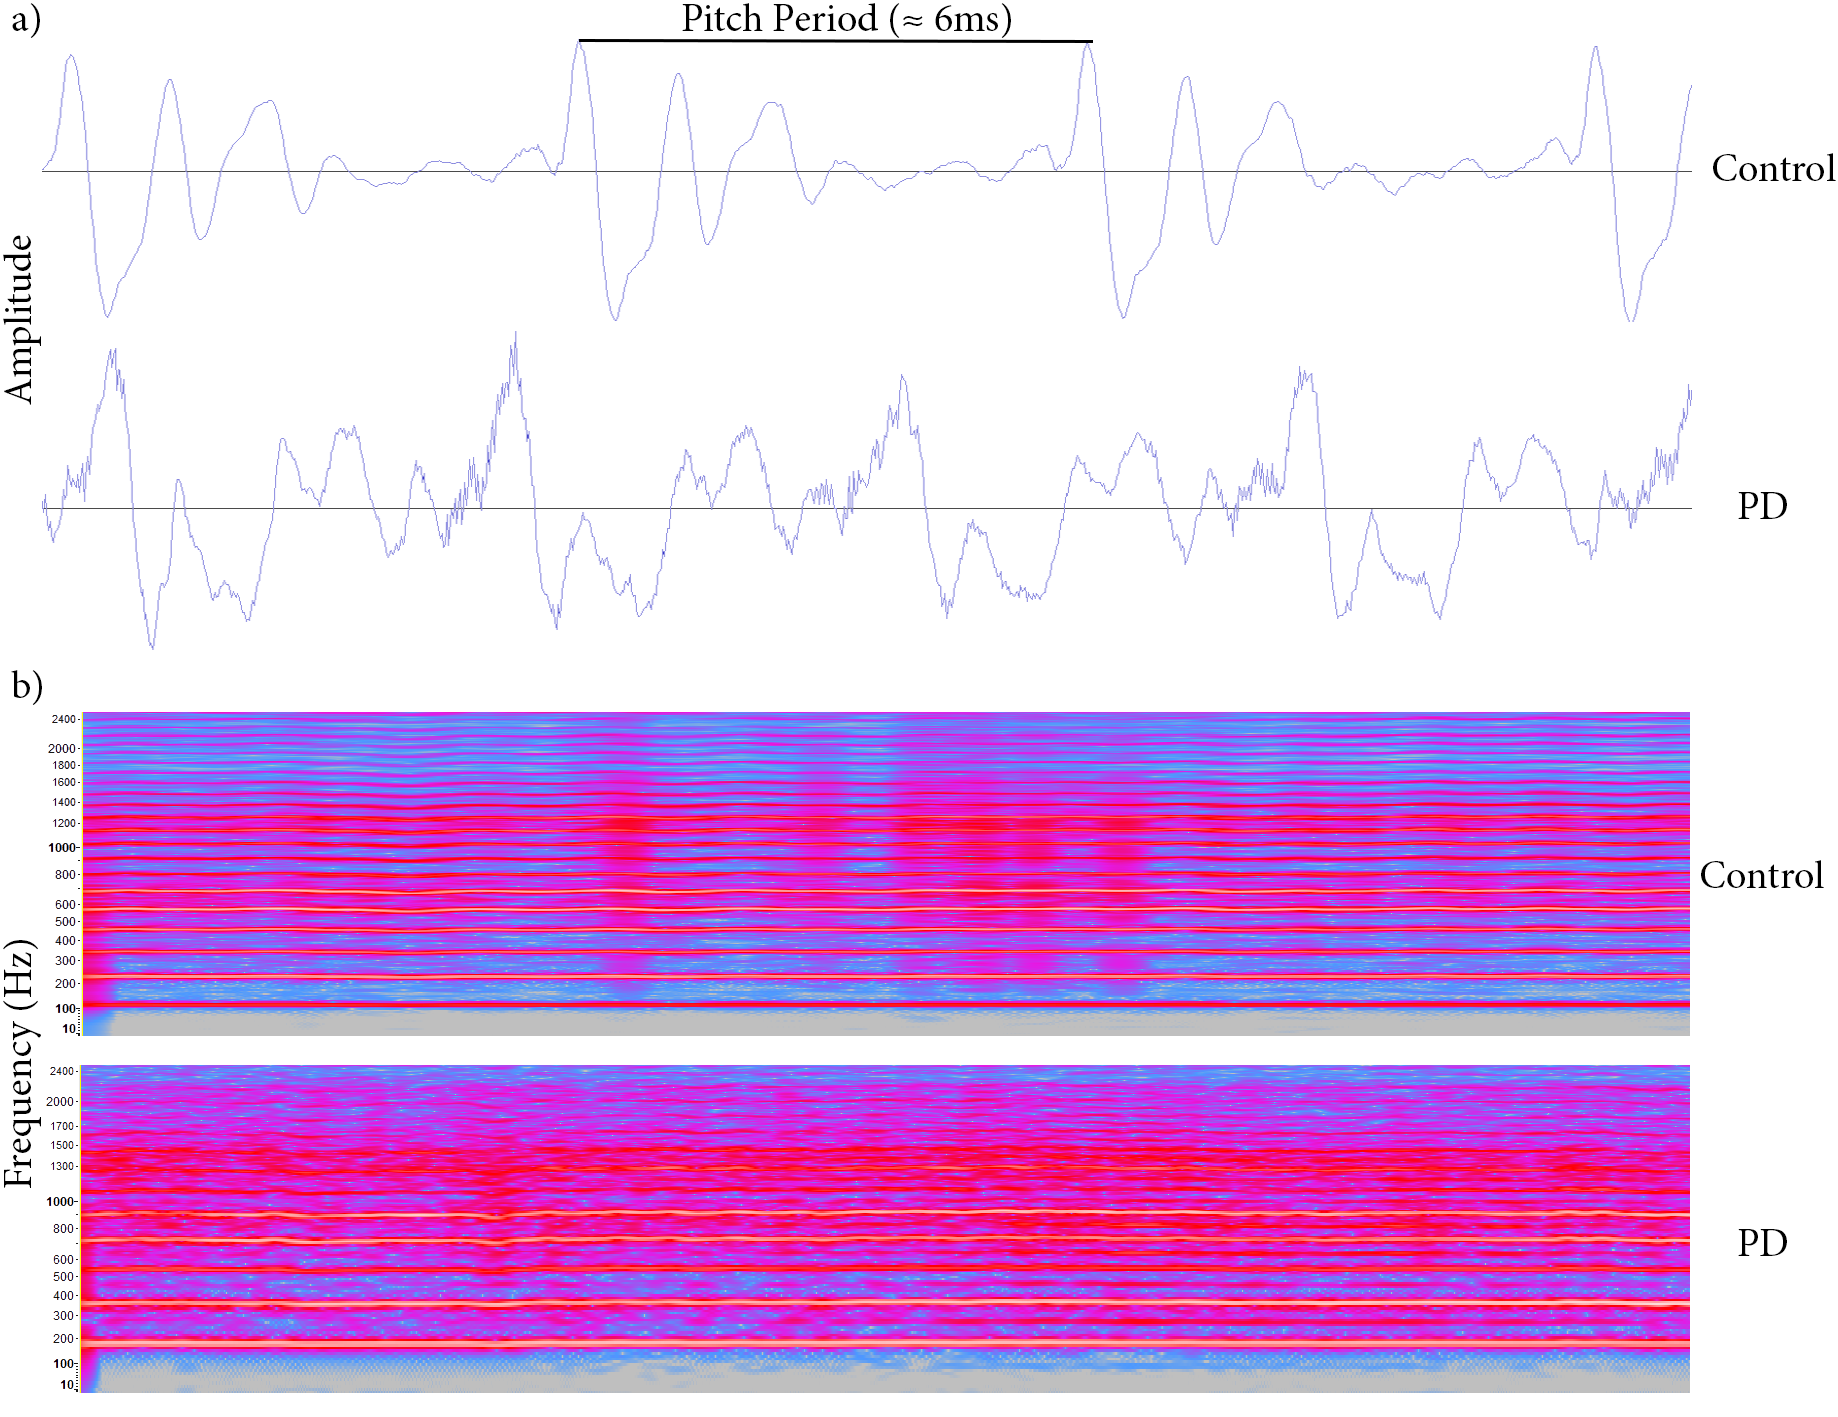
\includegraphics[width=1.2\linewidth]{timespectrogram.png}}
	\caption{A visualisation of prominent dypshonia in sustained vowel phonation on the time (above) and short-time frequency domain (below, Mel-scale~\cite{mfscale}). Cases are generally not as extreme and the natural variation in voice makes differentiation a difficult task.}
\end{figure}


Although changes in speaking patterns (dysarthia) are very perceivable to human ears, features such as slurring or hesitation can only be roughly estimated with current technologies. There are also a number of complexities involved in modelling \emph{spoken language}, with a wide variation of accents and styles. Hazan~et~al.~(2012)~\cite{hazan2012} investigates PD diagnosis on English and German sentences, however does not use any short-time features.  Hazan~et~al. also observes that machine learning models trained on the English speakers do not generalize well to the German speakers and vice versa. 

The Interspeech 2015~\cite{compareis15pd} competition featured a sub-challenge where the extent of PD dysarthria (as rated by the UPDRS) was to be estimated based on sentence and word pronunciations. The challenge dataset consists of pronunciations of isolated words and sentences from 50 patients in a controlled environment with a professional grade microphone. The best performing papers in this sub-challenge only managed Pearson correlations of 0.4 to 0.64 against neurologist diagnosis~\cite{hahm2015parkinson,grosz2015assessingis15,williamson2015segment}.

However recent works point to evidence that speech can be a powerful predictor given better signal processing approaches. Vasqeuz et~al.~(2015)~\cite{vasquez2015automatic} is able to enhance noisy PD speech data using a technique proposed in Wang~et~al.~(2007)~\cite{wang2007speechenhancement} which decomposes speech into signal and noise subspaces. Orozco~et~al.~(2015)~\cite{orozco2015voiced} quantifies the transitions between voiced and unvoiced speech and presents significantly better results compared to using voiced speech as in prior works.

\emph{Sustained vowel phonations} are the preferred method of quantifying dysphonia. Although features used in the general speech signal processing are applicable in dysphonia quantification, features developed specifically for dysphonia may be more robust as they are based on the non-linear model of speech production~\cite{splittledysphonia2009, splittlenonlinear2007}. Dysphonia specific features generally quantify the variation in each glottal cycle, relying on an an accurate fundamental frequency estimation algorithm~\cite{f0estimation}. 

\begin{highlight}
As dysarthria is difficult to quantify, dysphonia based signal processing methods currently show more promise.
\end{highlight}

Early dysphonia analysis is based on variations of jitter, shimmer and the harmonics-to-noise ratio. \emph{Jitter}~ measures the variation in the length of each glottal cycle, and \emph{shimmer}~\cite{shimmerjitter,jittertime} the variation in amplitude (volume). The harmonics-to-noise ratio (\emph{HNR})~\cite{HNRintro} measures the amount of noise in a signal, which correlates with the `hoarseness' or `breathiness' from an incomplete closure of the glottis.  The Glottal to Noise Excitation (\emph{GNE}) ratio was introduced by Michaelis~et.al~(1997)~\cite{gne} and is a more reliable measure of dysphonia than HNR~\cite{gneratio}. 

\label{dfadescription}
More recently, methods used in non-linear dynamical systems\footnote{Dynamical systems theory is used to describe the behaviour of deterministic systems which appear to exhibit unpredictable behaviour based on a number of initial conditions. Dynamical systems are often viewed as a stochastic process for the purpose of analysis.} have been shown to be effective to dysphonia quantification. Detrended Fluctuation Analysis (\emph{DFA}) was originally introduced by Peng~et~al.~\cite{dfa} as a measure of the autocorrelation of a signal. Little~et~al.~(2007)~\cite{splittlenonlinear2007} shows this correlates with the amount of turbulent airflow in speakers with dysphonia. Little~et~al.~(2007) also proposes Recurrence Period Density Entropy (\emph{RPDE}) which characterises the repetitiveness of a signal, which is generally lower for speakers with dysphonia due to jitter and shimmer. As the method does not rely on the detection of the fundamental frequency it may be more robust for dysphonic speakers. Little~et~al.~(2009)~\cite{splittledysphonia2009} builds upon RPDE to develop Pitch Period Entropy (\emph{PPE}) which is a better measure of the impaired control of pitch experienced by PD patients.

Tsanas~et~al~(2012)~\cite{tsanas2012novel} extends GNE to develop Vocal Fold Excitation Ratios (\emph{VFER}) and also introduces the Glottal Quotient (\emph{GQ}). GQ measures the standard deviation of the duration when the glottis is opened and closed and is founded on the principles of the DYPSA~\cite{dypsa} fundamental frequency estimation algorithm. We refer to Tsanas~(2012)~\cite{spoverview} for a more detailed summary of the signal processing involved.

Mel-Frequency Cepstral Coefficients (\emph{MFCC}) have long been used for speech recognition~\cite{mfcc}, and have also shown promise in detecting dysphonia~\cite{mfccml}. They are the most common and often the only feature used in speech recognition systems however lack interpretability and is very sensitive to noise~\cite{mfccrobust}. There are also a variety of feature sets used in general speech classification, such as the 6,368 in the 2013 Intespeech ComParE set~\cite{is2013}. Although not all of these features may measure dysphonia, they are effective in fields such as speaker trait classification and may be useful in complex machine learning models. The incidence of PD varies based on age, gender and race~\cite{ageracial,racial}, and it is likely that dysphonia presents itself differently depending on speaker traits. We refer to Eyben~(2015)~\cite{ostextbook} for a comprehensive description of these features as well as a summary of feature sets used in speech classification.

\subsection{Movement}\label{movementfeatures}
Despite a similar amount of literature existing in both movement and voice feature extraction, signal processing in the voice domain is more developed. Feature extraction for movement data diverges into a number of subfields, each developing different measurements for different sensors to quantify the extent of a movement disorder. Features are crafted specifically for dyskinesia\footnote{\emph{Dyskinesia} describes the presence of involuntary, often `jerky' movements.} and akinesia\footnote{\emph{Akinesia} is the impairment of voluntary movement.} quantification. The signal processing techniques used in movement disorder quantification are basic compared to methods in voice and EEG.

People with PD exhibit increased tremor, particularly in the 3.5-7hz range~\cite{duval2004detection} as well as distinct patterns of sway which can be quantified by recurrence analysis~\cite{palmerini2011tremor, posturalswaylongitudinal}. These are best measured when the subject attempts to stand as still as possible. Both IMUs and force plates are able to quantify this --- IMUs have the advantage of being cheaper and more accessible however have lower resolution and may not be spatially accurate. There has not yet been a study comparing the information content of the two. The amount of tremor can be easily quantified with a Fourier transform, and recurrence can be quantified with general signal processing techniques such as DFA (see \ref{dfadescription}).

It is also possible to quantify gait with IMUs. Barth~et~al.~(2011)~\cite{barth2011biometric} and Sijobert~et~al.~(2015) \cite{sijobert2015implementation} propose gait estimation algorithms for IMUs attached to the foot and shank respectively. It is also possible to estimate gait with handheld or in-pocket IMUs as done in Renaudin~et~al.~(2012)~\cite{renaudin2012step} and Diaz and Gonzalez~\cite{diaz2014step} respectively. However existing algorithms do not perform to the standards required to detect akinesia and are not very robust. Force Walkways and motion capture are more accurate alternatives for measuring gait however are more costly and only available in a clinical context. 

Although expensive and difficult to setup, motion capture presents the possibility of completely quantifying all movement related components. However, feature extraction has not evolved to take advantage of the additional information and a significant amount of training data would likely be required to realise its full potential. Das~et~al.~(2011)~\cite{das2011quantitative} uses motion capture on 4 PD and 2 control subjects, however does not explore any spatial features beyond what is provided by multiple accelerometers. Pose recognition in video is also an rapidly developing field which proposes similar capabilities to motion capture at a fraction of the cost. Current models are promising, however are not precise enough to be used in combination with akinesia detection.

\subsubsection{Smartphones}
Smartphones are becoming increasingly common, even in developing countries. As they contain a number of sensors such as accelerometers, microphones and cameras, they are a promising tool in \textit{telemedicine}, where PD can be remotely diagnosed or monitored. The universal nature of smartphones makes large PD datasets possible, with the 8,000 patient mPower~\cite{mpower} dataset used in this paper crowdsourced from smartphone users.

Smartphone studies generally use features presented in speech and accelerometer research, along with additional tests such as memory or tapping tasks~\cite{tapping}. However the resolution and accuracy of smartphone sensors greatly varies and introduces significant noise to the data. The influence of smartphone models on results has yet to be investigated, and it is unknown whether generalizing between phones is possible. Smartphone step and motion mode recognition\footnote{\emph{Motion mode recognition} involves classifying whether the user has their phone in their pocket, hand, bag  }~\cite{motionmoderecognition, li2010multimodal} is a similar research area, however techniques are less applicable as measures are often more coarse.


Little~et~al.~(2009)~\cite{splittledysphonia2009} provides evidence that a high quality microphone is not required to classify dysphonia, obtaining good results on a dataset of 33. Brunato~et~al.~(2013)~\cite{smartphonemjfoxlion}, Boussios~et~al.~(2013)~\cite{smartphonemjfoxB} and Arora~et~al.~(2014)~\cite{arora2014high} also manage to obtain good results with simple accelerometer based features. However all of these models have been tested on small datasets, which are prone to overfitting on cross validation~\cite{overfittingcv}, bias and uninformative predictors~\cite{freedmanparadox}. 


Zhan~et~al.~(2016)~\cite{zhan2016high} conducts a smartphone feasibility study on the largest dataset to date --- 121 PD and 105 control. Participants were recruited into the study and asked to asked to conduct tasks such as walking, saying `aaaah...' and alternated tapping~\cite{tapping}. However, Zhan~et~al. obtained results barely above the conditional baseline when predicting on features from all tasks (71\% accuracy). This result is also especially poor considering that the mean (standard deviation) age of PD subjects was 57.6 (9.4) and control 45.5 (15.5). A similar result may be obtained by a model classifying with age alone. This result is in direct contradiction with the previous works such as Arora~et~al.~(2014)~\cite{arora2014high} which reported 98.0\% accuracy on very similar accelerometer features. It is evident that reported results must be taken with a grain of salt. A possible cause is that Zhan~et~al. does not control the android smartphone used, hence the sensor data collected varies significantly between devices. Zhan~et~al. also uses very basic features to quantify speech, neglecting the state of the art speech signal processing features used in other works~\cite{ostextbook, spoverview}. 


\subsection{EEG}
Electroencephalogram (EEG) signal processing presents an interesting challenge as the characteristics of an EEG signal are less well understood compared to speech and motion. Although many features have been crafted specifically for diagnosis of PD and Alzheimers with EEG~\cite{eegnonlinearpd, eegalzheimers}, this section will only cover those which may be applicable to speech and movement.

A variety of EEG signal processing techniques are inspired by non-linear dynamical systems theory. It is believed that EEG signals are generated by non-linear coupling interactions between neuronal populations~\cite{eegalzheimers}. Patients suffering from neurodegenerative disorders often exhibit decreased complexity in EEG patterns, believed to be caused by the a decrease in  non-linear cell dynamics~\cite{jelles1999decrease}. Features developed with EEG signal processing aim to characterise the dynamic structure of this system. As these features are not inspired by human senses, these features are the very promising for the task of measuring the presence of symptoms undetectable by a neurologist. 

\begin{highlight}
The nature of features related to EEG make them very promising for the task of measuring the presence of symptoms undetectable by a neurologist.
\end{highlight}

The \emph{Lyapunov Exponents} quantify the divergence of two systems with infinitesimally similar initial conditions. The Largest Lyapunov Exponent (\emph{$L_1$}) characterises the chaos\footnote{Chaos refers to the sensitivity of a dynamic system to its initial conditions.} or rate of divergence of a system and is commonly estimated with Rosenstein's algorithm~\cite{rosenstein1993practicallyapunov} which reconstructs the system's dynamics using a time delay technique\footnote{Additional Lyapunov exponents generally require known equations describing the system~\cite{lyapunovall}.}. The $L_1$ has long been used in the EEG analysis of sleep and as a feature for machine learning~\cite{eeglyapunov1, eeglyapunov2}. More recently, the $L_1$ has been applied to analyse the non-linearity of speech~\cite{banbrook1999speechlyapunov, kokkinos2005nonlinearlyapunov}, gait and balance ~\cite{dingwell2000nonlinearlyapunov, howcroft2014analysisgaitlyapunov, liu2015analysislyapunov}.

%The term as coined by Mandelbrot in 1967~\cite{mandelbrot1967long}

The \emph{fractal dimension} is another measure commonly used in the analysis of EEG and other dynamical systems along with the LLE. It represents the ratio of the log change in detail to log change in scale of a signal\footnote{The coastline paradox is the observation that as you measure a coastline with increasingly smaller measuring sticks, the measured coastline length will increase. The \emph{fractal dimension} would measure the ratio of change in length as of the `stick' used to measure the coastline is made shorter.}~\cite{mandelbrot1967long}. A higher value implies a more complex signal and the fractal dimension of an EEG signal with open vs closed eyes and normal vs epileptic states are observably smaller~\cite{eegfractal, seizuredimensions}. The fractal properties exhibited in neuronal control are reflected in heartbeat and gait~\cite{fractalgait} with force plate data from elderly and Parkinsonism subjects showing a significant increase in fractal dimension compared to healthy young subjects~\cite{hfdcop, fractalpd, fractalbalance}. Esteller et~al.~\cite{fractaldimensions} compares algorithms estimating the fractal dimension of signals.

The \emph{Hurst} exponent characterises the autocorrelation or long-range dependence of a signal~\cite{hurst1965long}. For self-similar signals, the Hurst exponent relates directly to the fractal dimension. In general the measures are independent with the Hurst exponent characterising the global rather than local properties of a signal~\cite{hurstfractal}. A Hurst exponent less than 0.5 characterises the signal `switching' between high and low values, 0.5 characterises random walk like behaviour, and values greater than 0.5 imply positive autocorrelation. Like fractal dimension, the Hurst exponent is a valuable tool in the analysis of gait and balance~\cite{duarte2000fractal}. Detrended Fluctuation Analysis (DFA) is essentially a generalisation of the Hurst exponent for non-stationary\footnote{Non-stationary systems are those with properties which evolve over time.} stochastic processes and has been applied in dysphonia diagnosis~\cite{splittlenonlinear2007}. Although DFA is the more robust measure, the disparity between the measures may reveal information on the dynamics of the system.

\emph{Fisher Information} is a measure relating to the uncertainty of measuring a variable (signal) about the unknown parameters modelling its distribution~\cite{fisherentropy}. It is applicable in quantifying non-linear dynamics~\cite{fisherinfo} and is often applied in the analysis of EEG~\cite{martin1999fisherinfoeeg}. General entropy will not differentiate two sequences where the frequency of each variable is the same, however the sequences 0,0,0,0,1,1,1,1 and 0,1,0,0,1,1,0,1 are clearly generated by different stochastic processes. \emph{Approximate} and \emph{sample entropy} are similar measures which aim to quantify this unpredictability in a signal~\cite{apsampentropy, apentropy}. The multi-scale sample entropy~\cite{multiscaleentropy} is especially powerful tool in the analysis of biological signals~\cite{samplegaitmulti, sampleheart}. Although these are a prominent feature in EEG analysis, they are rarely used in voice and movement analysis. 


\subsection{Summary of Features}
This section summarises all the features covered in previous sections which are used in the construction of models presented in this thesis, which are based on audio and accelerometer signals. The libraries and parameters used to implement are covered in detail in section \ref{implementation}. Features are organised by field of introduction or by the field they are most commonly applied in. All relevant general and EEG features are extracted for both the audio and accelerometer models used in this thesis. Additionally, RPDE and DFA are used as a feature for the accelerometer data.

\label{featuresummary}
% \centering
\bgroup
\def\arraystretch{1.3}%
\begin{longtable}{r p{114mm}}
\caption{Features and techniques which are applicable to any signal processing problem.}\\
\multicolumn{2}{c}{\specialcellbold{General Signal Processing}} \\
\toprule
Moments & Statistical features --- mean, variation, skewness, kurtosis, etc.\\
Crossing Rate & Rate the signal oscillates around a value --- usually zero or the mean.\\
\specialcellright{Information\\ \hspace{1em}Theoretic} & Entropy, mutual information, cross-correlation and related measures based on the information content of signal. \\
Spectral Flux & Rate at which the power spectrum changes\\
Fourier & Transforms the signal from time domain to frequency domain. Quantifies the \textit{power} of a signal at a given frequency.\\
Wavelet & A variation of the Fourier transform with a different bases, allowing it to quantify both time and frequency\\
\specialcellright{\hspace{3em}Energy\\Operators~\cite{tkeo}}& Quantifies the instantaneous amplitude and frequency of a signal. Common operators are Teager-Kaiser (TKEO) and Squared (SEO) \\
\bottomrule 
\end{longtable}

\begin{longtable}{r p{114mm}}
	\caption{Dysphonia signal processing generally quantifies the variation in each glottal cycle during speech production}\\
\multicolumn{2}{c}{\specialcellbold{Speech -- Dysphonia}} \\
\midrule
 \specialcellright{Power\\Cepstrum} & From the inverse Fourier domain. Commonly taken in the Mel-log scale~\cite{mfscale}, resulting in the MFCC~\cite{mfcc}. Minimal interpretability, however is the primary feature used in speech recognition~\cite{mfccml}. \\
Pitch~\cite{f0estimation} & Although obtainable with a Fourier transform, pitch often refers to estimating the exact duration of each glottal cycle.\\
Loudness & The volume of a sound in relation to human hearing. Only meaningful if recording setup is strictly controlled.\\
Formants & The resonance frequencies of an audio sample.\\
HNR~\cite{HNRintro,HNRperiodic} & Measures the ratio of noise in a voiced signal (signal to noise)\\
Jitter~\cite{jittertime} & Measures of the variation between the length of each glottal cycle. \\
Shimmer~\cite{shimmerjitter} & Measures of the variation of amplitude between each glottal cycle. \\
LPCC~\cite{lpcc} & Coefficients of an \textit{autoregressive} model which measures how well a signal can be modelled linearly by its previous values.\\
GNE~\cite{gne} & An extension of HNR by Michaelis et~al.~\cite{gne} to improve reliability in dysphonia quantification\\
VFER~\cite{tsanas2012novel} & An further extension of HNR, building upon the theory of GNE.\\
EMD-ER~\cite{EMDER} & Another technique developed based on non-linear speech theory to quantify signal to noise\\
GQ~\cite{tsanas2012novel} & Measures standard deviation of duration the glottis is opened vs closed.\\
DFA~\cite{splittlenonlinear2007, dfa} & Detrended Fluctuation Analysis. A generalisation of the Hurst exponent which measures the self-similarity of a time series.\\
RPDE~\cite{splittlenonlinear2007} & Measures the repetitiveness of a signal, specifically designed with non-linear speech as the target.\\
PPE~\cite{splittledysphonia2009} & Measures the variation in successive glottal cycles.\\
\specialcellright{\hspace{1.9em}Wavelet\\Measures~\cite{sptsanastelemonitor2010}} & A set of 180 measures for dysphonia based on wavelet transforms to the $f_0$ of speech introduced by Tsanas~et~al.~(2011)~\cite{tsanas2011nonlinear}.\\
\specialcellright{GeMAPS~\cite{geneva}} & A minimal acoustic feature set of 58 or 87 (eGeMAPS) parameters that performs well in general speech classification~\cite{ostextbook}.\\
\specialcellright{\hspace{1.3em}Interspeech\\ComParE~\cite{compareis13featureset}} & An exhaustive 6,368 feature set for general speech classification~\cite{ostextbook}. Feature/dimensionality reduction generally improves performance unless data is plentiful.
%\\\specialcellright{Hammarberg\\ \hspace{0.2em} Index~\cite{hammarberg1980perceptual}} & The ratio of the strongest energy peak from 0-2kHz versus 2-5kHz. The \textit{Alpha Ratio} is similar, measuring the largest peak 50Hz-1kHz versus 1kHz-5kHz.\\
\\
\bottomrule
\end{longtable}


\begin{longtable}{r p{114mm}}
	\caption{There are few movement specific features, with most based on simple measures of postural sway or irregular gait.}\\
\multicolumn{2}{c}{\specialcellbold{Movement}} \\
\midrule
\specialcellright{\hspace{2.5em}Fourier\\\hspace{2.7em}Bands} & The power in bands such as 3.5hz-7hz compared to 7hz-12hz are the primary features used to detect Parkinsonism tremor.\\
Jerk~\cite{jerkfeature} & The change in acceleration. The jerk signal may be more effective when combined with certain signal processing methods.\\
\specialcellright{Sway\\Area} & Simple measures such as bounding ellipse can quantify the amount of sway. A 95\% CI is often taken to remove outliers.\\
\specialcellright{Cadence\\Measures} & The steps per minute, variation in time taken for each step, difference between left and right stride times.\\
\specialcellright{\hspace{1em}Stride\\Measures} & The length of each step and variation in step lengths. This was not measured as leg length is not available in the dataset used~\cite{diaz2014step}.
\\ 
\bottomrule
\end{longtable}



\begin{longtable}{r p{114mm}}
	\caption{EEG signal processing is often based on dynamical systems theory. These features may be effective in detecting the presence of symptoms invisible to neurologists.}\\
\multicolumn{2}{c}{\specialcellbold{EEG}} \\
\midrule
\specialcellright{\hspace{3.6em}Hjorth\\Parameters~\cite{hjorth}} & Three simple statistical measurements of a signal which have been used as features in EEG and IMU models~\cite{hjorthsmartphone}.\\
\specialcellright{\hspace{2em}Lyapunov\\Exponents~\cite{rosenstein1993practicallyapunov}} & Characterises the divergence of systems with close initial conditions. The largest exponent (LLE)~\cite{dingwell2000nonlinearlyapunov} is most commonly used. \\
\specialcellright{\hspace{3.3em}Fractal\\Dimension~\cite{mandelbrot1967long}} & A measure of how the detail in a signal changes with the scale at which it is measured. The Higuchi~\cite{hfd} and Petrosian~\cite{petrosian1995kolmogorov} fractal dimensions are used in this thesis.\\
\specialcellright{\hspace{3.2em}Hurst\\Exponent~\cite{hurst1965long}} & Characterises self-similarity. DFA is a generalisation of the Hurst Exponent and is robust to non-stationary signals. The difference in measurements may be informative.\\
\specialcellright{Fisher Info~\cite{fisherentropy}} & Quantifies the non-linear dynamics in the system generating a signal.\\
\specialcellright{\hspace{1.1em}Ap/Samp\\Entropy~\cite{apentropy}} & Approximate and sample entropy quantify the unpredictability of a signal. Multiscale entropy increases information content~\cite{multiscaleentropy}.\\
\specialcellright{\hspace{2.9em}SVD\\Entropy~\cite{svdentropy}} & A measure of complexity. The entropy of the orthogonal vectors from singular value decomposition needed to describe the signal.
\\
\bottomrule
\end{longtable}


\egroup
% \end{table}
\section{Machine Learning}
\label{machinelearning}
\begin{highlight}
Fundamentally, the goal of machine learning is to use past data to make accurate predictions about new data. 
\end{highlight}

Machine Learning tasks can be classified as classification or regression, and supervised or unsupervised. Classification involves predicting the \textit{class} of a datapoint --- for instance, distinguishing PD from control --- whereas regression involves predicting a numerical value, such as the UPDRS motor scores. In supervised learning, the data is \textit{labelled} with the ground truth --- i.e, whether the patient has PD --- whereas an unsupervised model must find patterns in the data without any prior knowledge. This section will focus specifically on \emph{supervised binary classification} (two classes). 


Supervised binary classification can be viewed as `learning' a model which given a set of numerical input features, predicts a class 0 or 1. This can be visualised as a function $f : \mathbb{R}^d \mapsto \{0,1\}$ where $d$ is the number of features used in the model. The edge where the $f$ transitions from zero to one is denoted the decision boundary (or `hyperplane') which partitions the data into the two classes. 


\begin{figure}[h]
\label{binaryclass}
\centering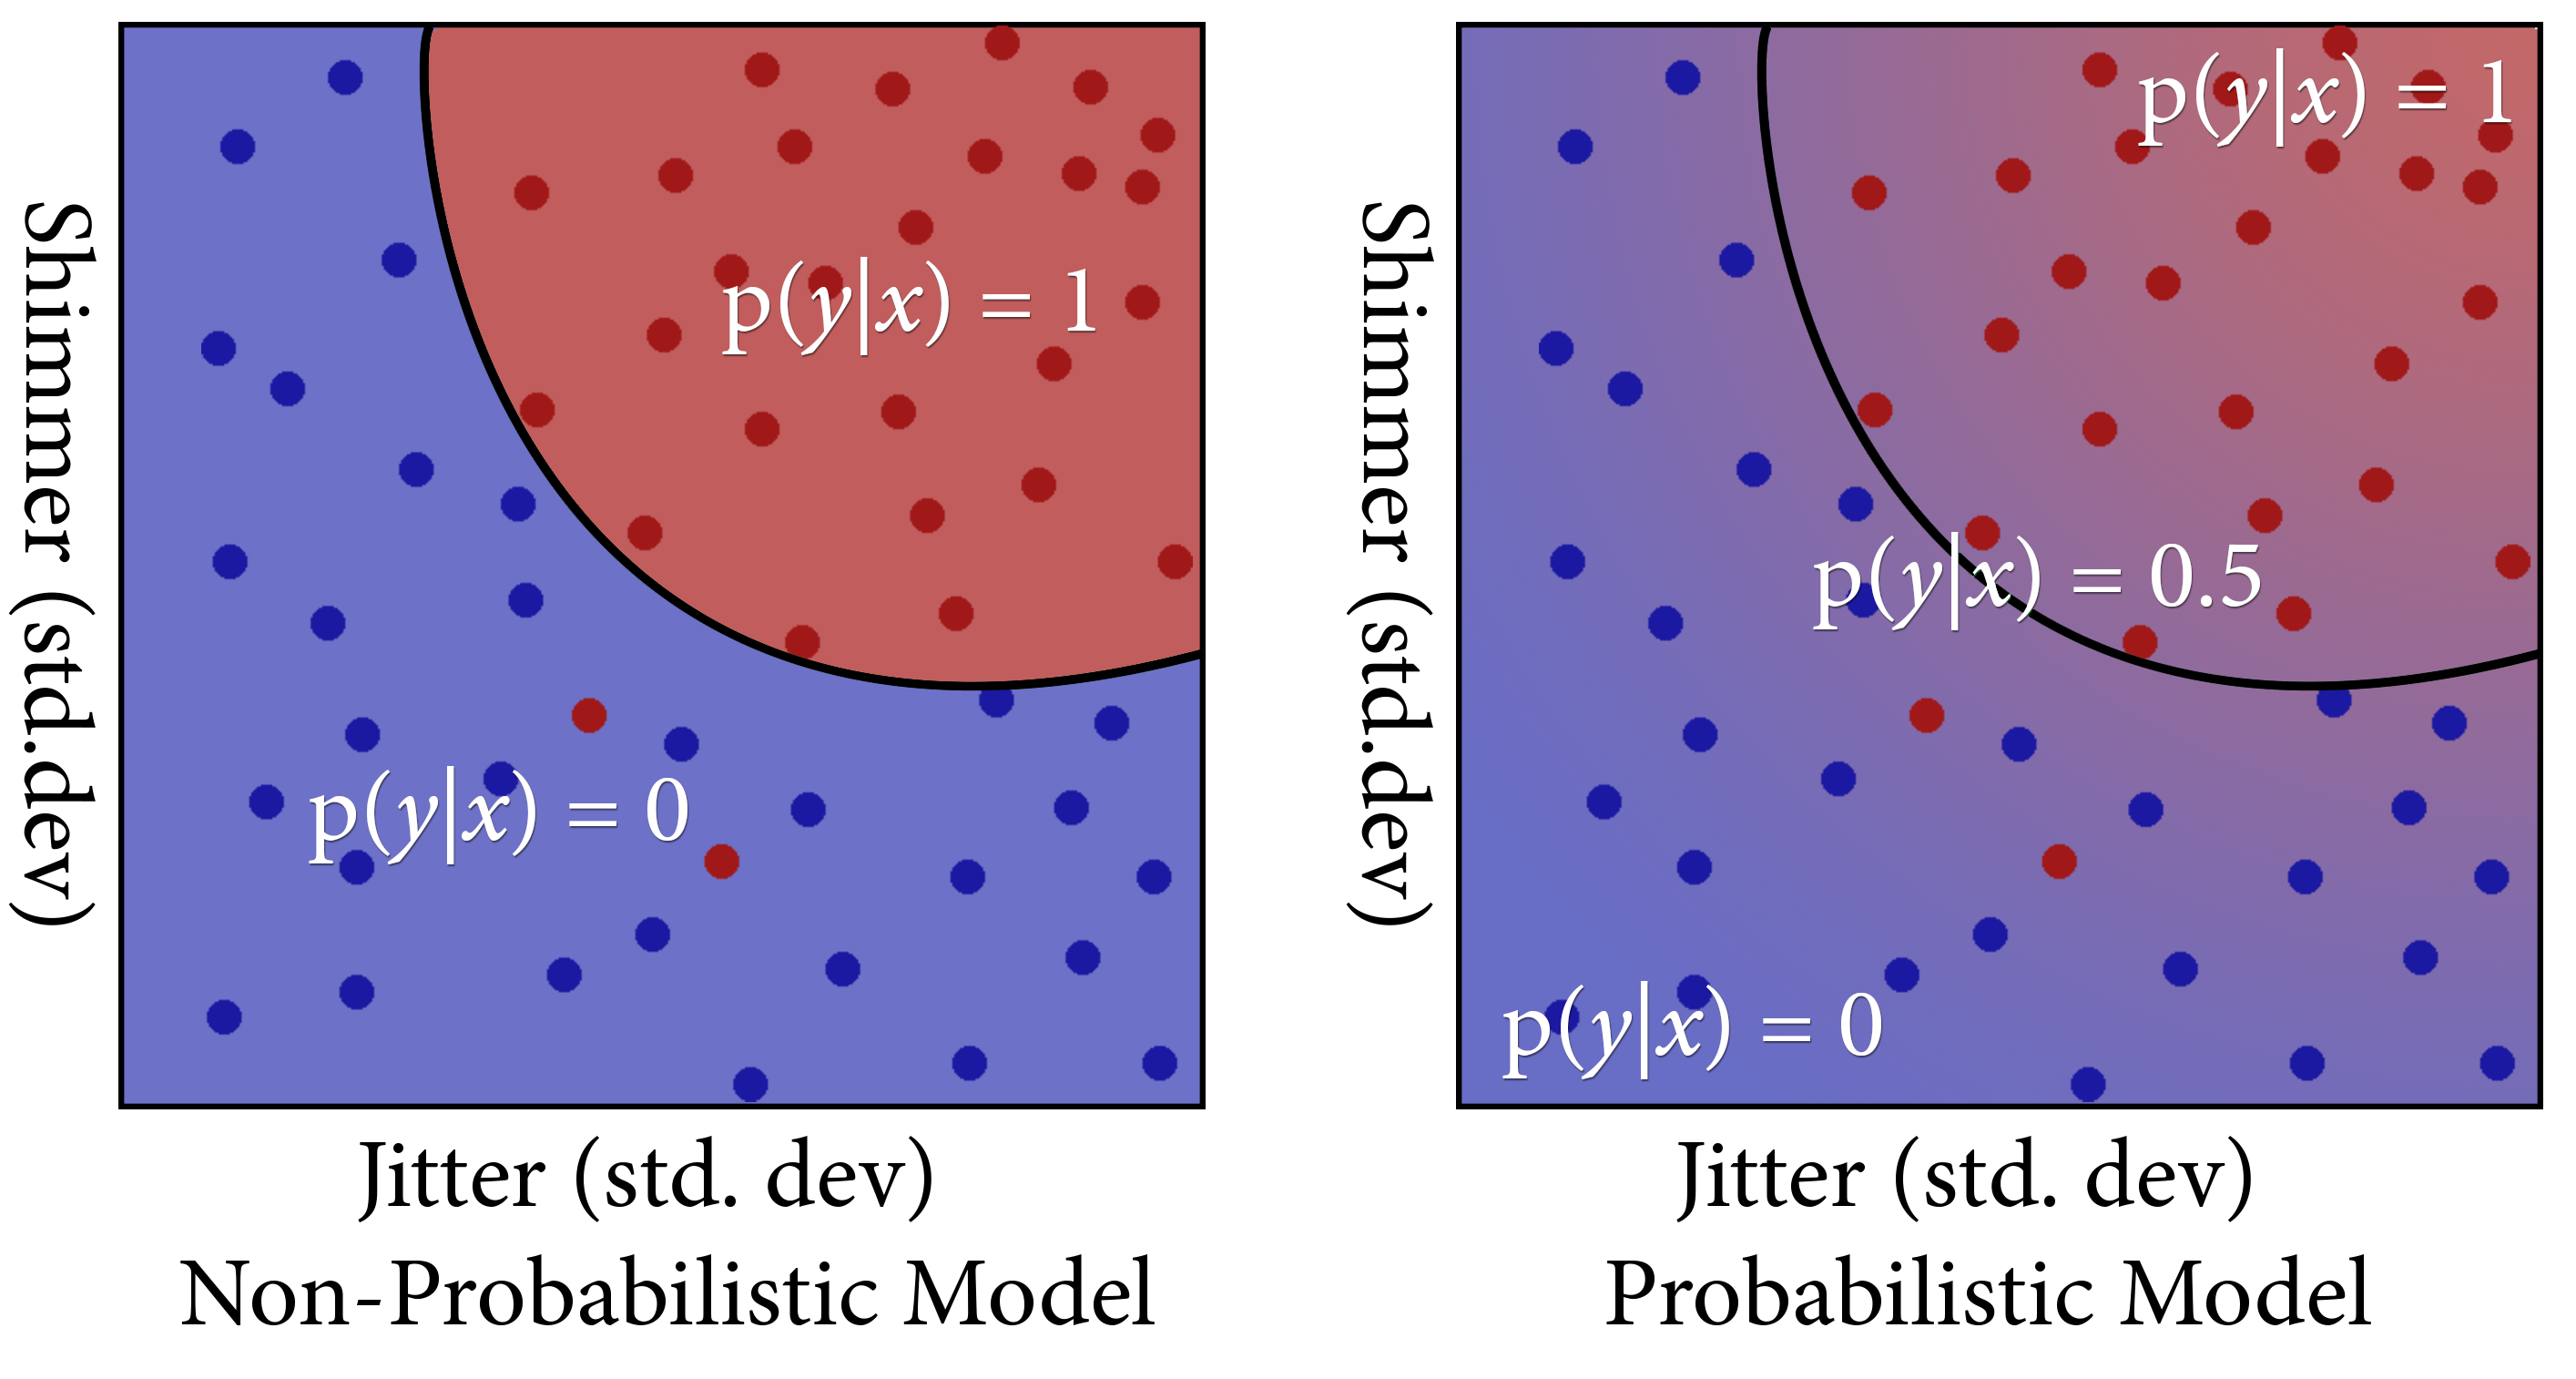
\includegraphics[width=0.7\linewidth]{binaryclassification2.png}
\caption{A visualisation of binary classification with two features. Data is rarely as `clean' as this artificial example.}
\end{figure}

Traditional machine learning models were built on statistical foundations. The mathematical backing these models are solid and the models well understood. However, the mathematics of these models were developed on assumptions that are rarely satisfied with real world data. Models such as deep neural networks have started to rise to popularity recently due to their modelling power. However the behaviour of deep neural networks are poorly understood and difficult to analyse.    

Most models have strengths in different areas, and very rarely does a model strictly dominate another. The choice of model is often informed by the data. For example, models like deep neural networks may perform well when data is plentiful, however in small datasets the very simple decision tree may greatly outperform neural networks\footnote{These will be explained in section \ref{traditionalmodels} and \ref{neuralnetworkintro}}.



\begin{highlight}
There is no `best' model --- the choice of model is informed by the data.
\end{highlight}

The predictive error in any model can be decomposed as \emph{irreducible error}, \emph{bias} and \emph{variance}. Irreducible error occurs when the features used are too noisy\footnote{\emph{Noisy} in the context of machine learning of signal processing relates to the inherent variance of a measure. An inaccurate, low quality sensor can be considered `noisy'.} or unrelated to accurately predict the data. An optimal model cannot achieve beyond this irreducible error. Bias describes a model `fitting' the data poorly and is evident in a model with low accuracy. Variance describes how `unstable' a model is --- a model with high variance may score 100\% accuracy but generalize poorly to new data. A model with high variance is essentially predicting results by `memorisation.' Fitting a model with high variance is often known as \emph{overfitting}. The bias-variance tradeoff~\cite{biasvarnn} is a fundamental problem in machine learning, describing the difficulty in reducing bias without increasing variance and vice versa. 

Models often have one or more adjustable parameters to balance bias and variance. These parameters are tuned with intuition combined with some form of search~\cite{gridsearch, tpe}. 

\begin{figure}[h]
\label{overfitex}
\centering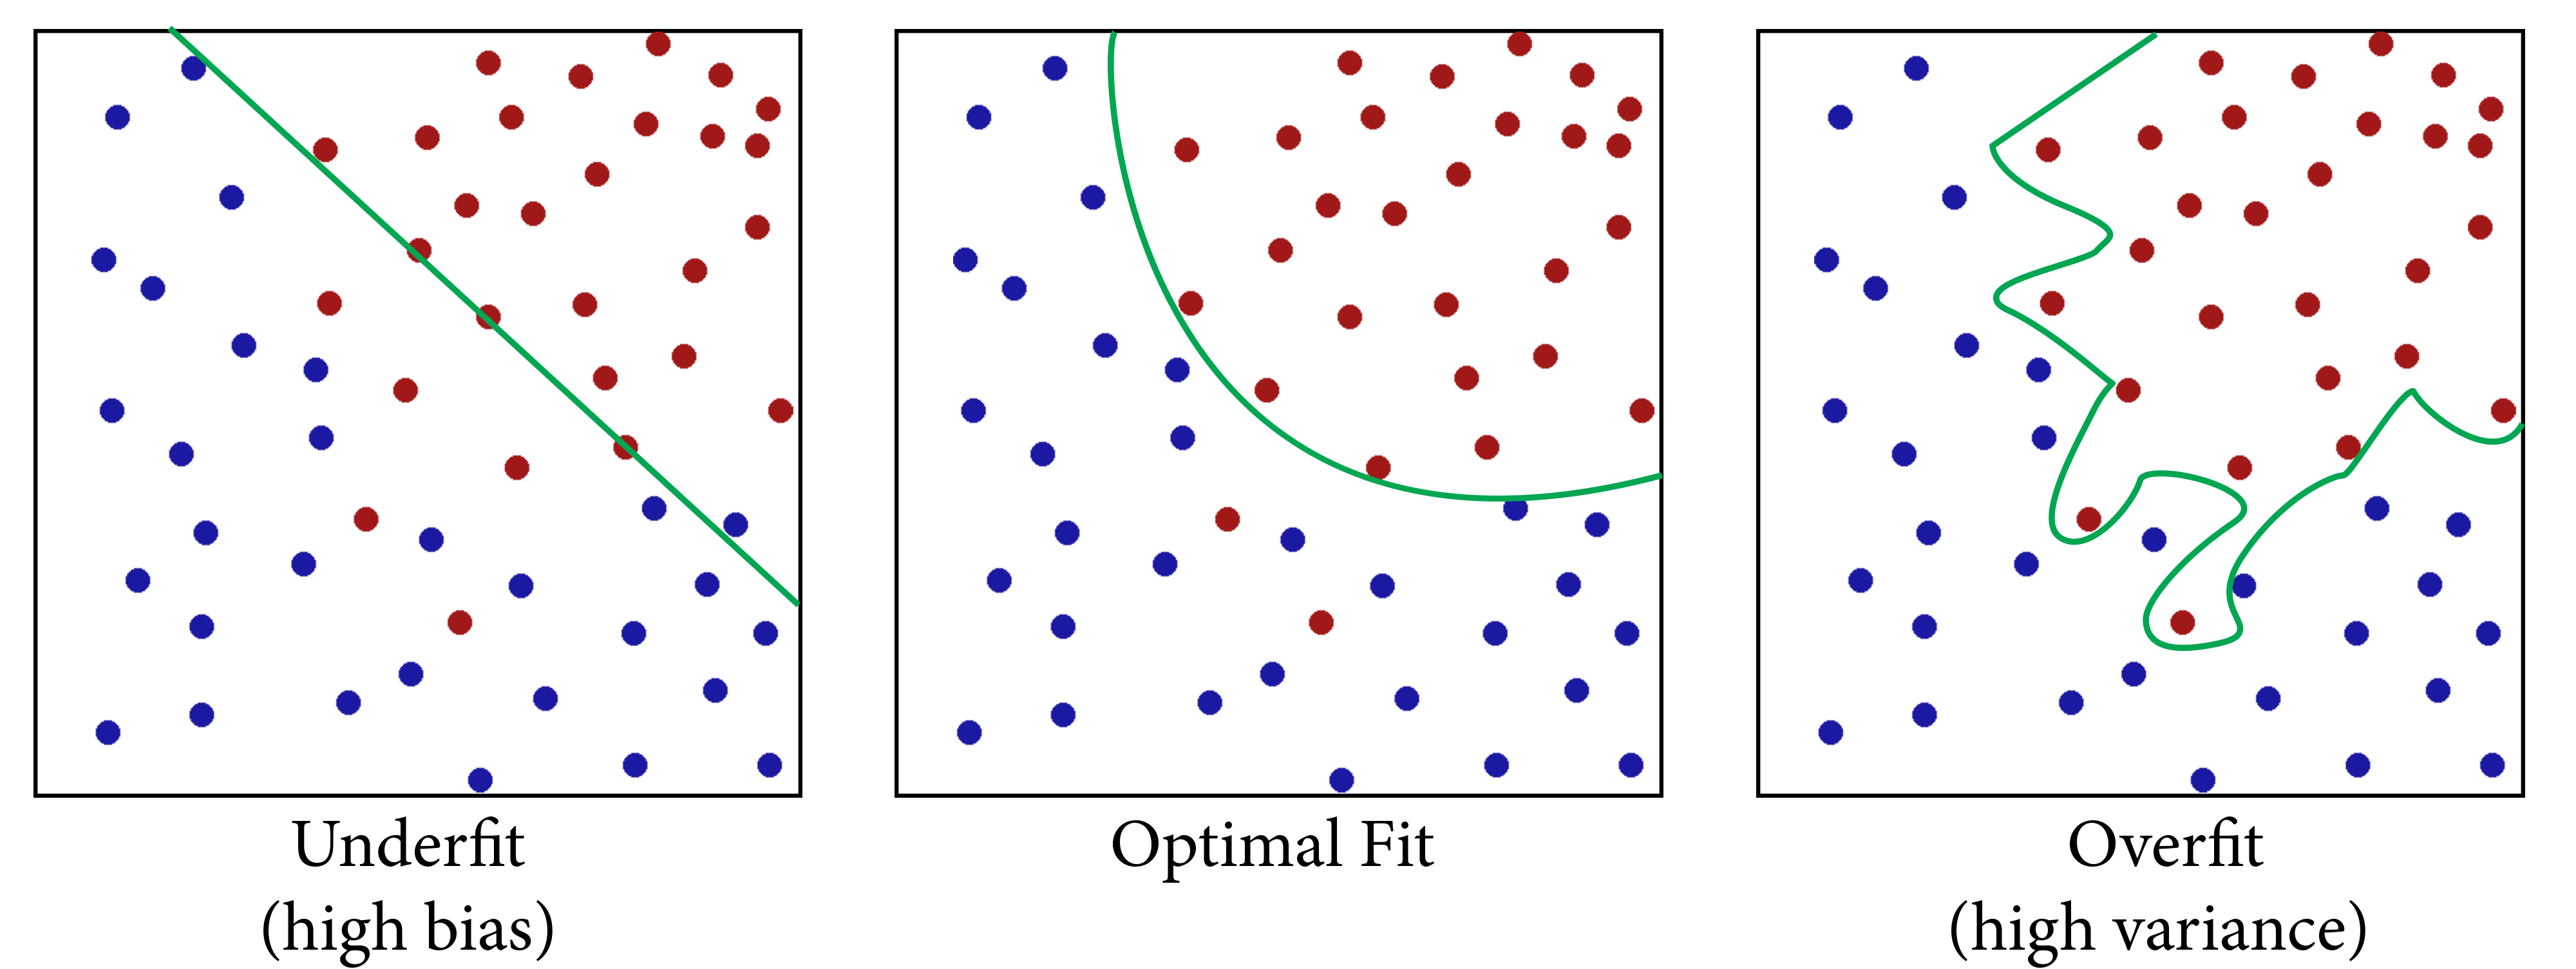
\includegraphics[width=1\linewidth]{overfit2.png}
\caption{Machine learning models and their parameters must be carefully chosen to ensure the optimal fit.}
\end{figure}

Overfitting is a major issue in machine learning as data is limited and models are often too complex to analyse. Visualising and detecting overfit may be simple when fitting a function in two dimensions, however it is significantly more difficult when the input has thousands of dimensions. A model that has overfit will appear to predict the data well, however fails to generalize to new data. Cross Validation is the gold standard in machine learning when it comes to model evaluation and recognising overfitting however it is not uncommon to find textbook examples which apply it incorrectly. Cross validation and other techniques used for model evaluation will be discussed in detail at section \ref{detectoverfit}. Like any statistics based field, careful analysis of the results is required and unfortunately this of often neglected in machine learning literature.


The following sections will cover three common models, random forest classifiers, support vector machine and neural networks. The mathematical formulation of these models is abstracted in favour for intuition behind their behaviour. We refer to Bishop~et~al.~(2005)~\cite{prml} for a more formal description of these models.

 
\subsection{Traditional}
\label{traditionalmodels}
Traditional models are the approach favoured in current literature~\cite{review2013} due to the limited data and their interpretability. The two most popular models used are \emph{Random Forests} (of decision trees) and Support Vector Machines (\emph{SVM}). Both of these are suitable for small datasets as they are relatively resistant to the curse of dimensionality. However both are also non-probabilistic classifiers\footnote{In general. Methods of generating pseudo-probability with SVMs have been proposed~\cite{svmprobabilistic}}. There exists models which are inherently probabilistic such as Gaussian Processes however they are less commonly used as they generally offer lower performance than decision boundary based classifiers.

\emph{Random Forest}~\cite{randomforests} classifiers are derived on the concept of Bootstrap Aggregation  (\textit{bagging})~\cite{bagging} where the results of multiple models are aggregated to obtain better performance than any of the constituent models alone. Random forests aggregate \emph{Decision Trees} which are one of the simplest and most common approaches to data mining and machine learning. 

\begin{figure}[h]
\label{decisiontree}
\centering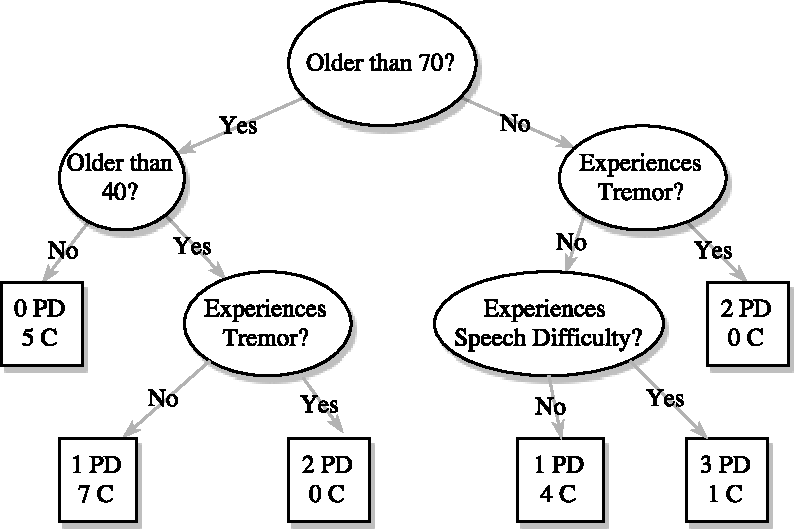
\includegraphics[width=0.8\linewidth]{decisiontree.pdf}
\caption{A simple Decision Tree with cutoff depth 3. Data is split by rules until a leaf contains only one class exists or a cutoff criterion is satisfied.}
\end{figure}

Decision Trees are simple to interpret and are robust against high dimensional data. However, determining the optimal decision rules at each node as well as the optimal cutoff criterion is a NP-complete problem. Decision rules are often developed based on greedy algorithms related to information criterion or search. A deep decision tree is prone to overfitting whereas a shallow one underfits.

Random Forests correct for the tendency of decision trees to overfit and provide robust and consistent results regardless of hyperparameters. The two hyperparameters are the number of trees to aggregate over and the number of features used in the search to split each branch of the tree. If the number of trees used is greater than the `complexity' of the problem, additional trees will not affect results~\cite{treesinaforest}. The square root of the number of features for classification is recommended by Breiman~\cite{randomforests} and is commonly used in most applications. Hence it is rare to perform hyperparameter tuning on random forests.

\begin{highlight}
Random forests provide robust and consistent results without the need for hyperparamter tuning.
\end{highlight}

\emph{Support Vector Machines}~\cite{svm} are built on the concept of creating the optimal decision boundary. The motivation is to create decision boundary which maximises the margin\footnote{The \emph{margin} is the smallest distance between the decision boundary and any of the samples} between different classes. This can be computed by solving a Lagrangian, however, this is only mathematically possible with a linear decision boundary. As most problems are not linear, the \emph{kernel trick} is used to transform the data into a linear space.


A kernel is a measure of similarity between two data points, and the kernel trick transforms the raw input into the feature space of the kernel\footnote{Kernels perform the same role as basis functions in linear regression}. Non-linear kernels enable a SVM to fit a non-linear function however the exact non-linearity in the data is rarely known. There are uncountably many kernels, and kernels such as the Radian Basis Function (RBF), Fisher and Polynomial are commonly used\footnote{There is rich literature in developing new kernels however these are rarely applied.}. Kernels generally have adjustable parameters, such as the degree and constant coefficient for polynomial kernels. 

\begin{figure}[h]
	\label{svm}
	\centering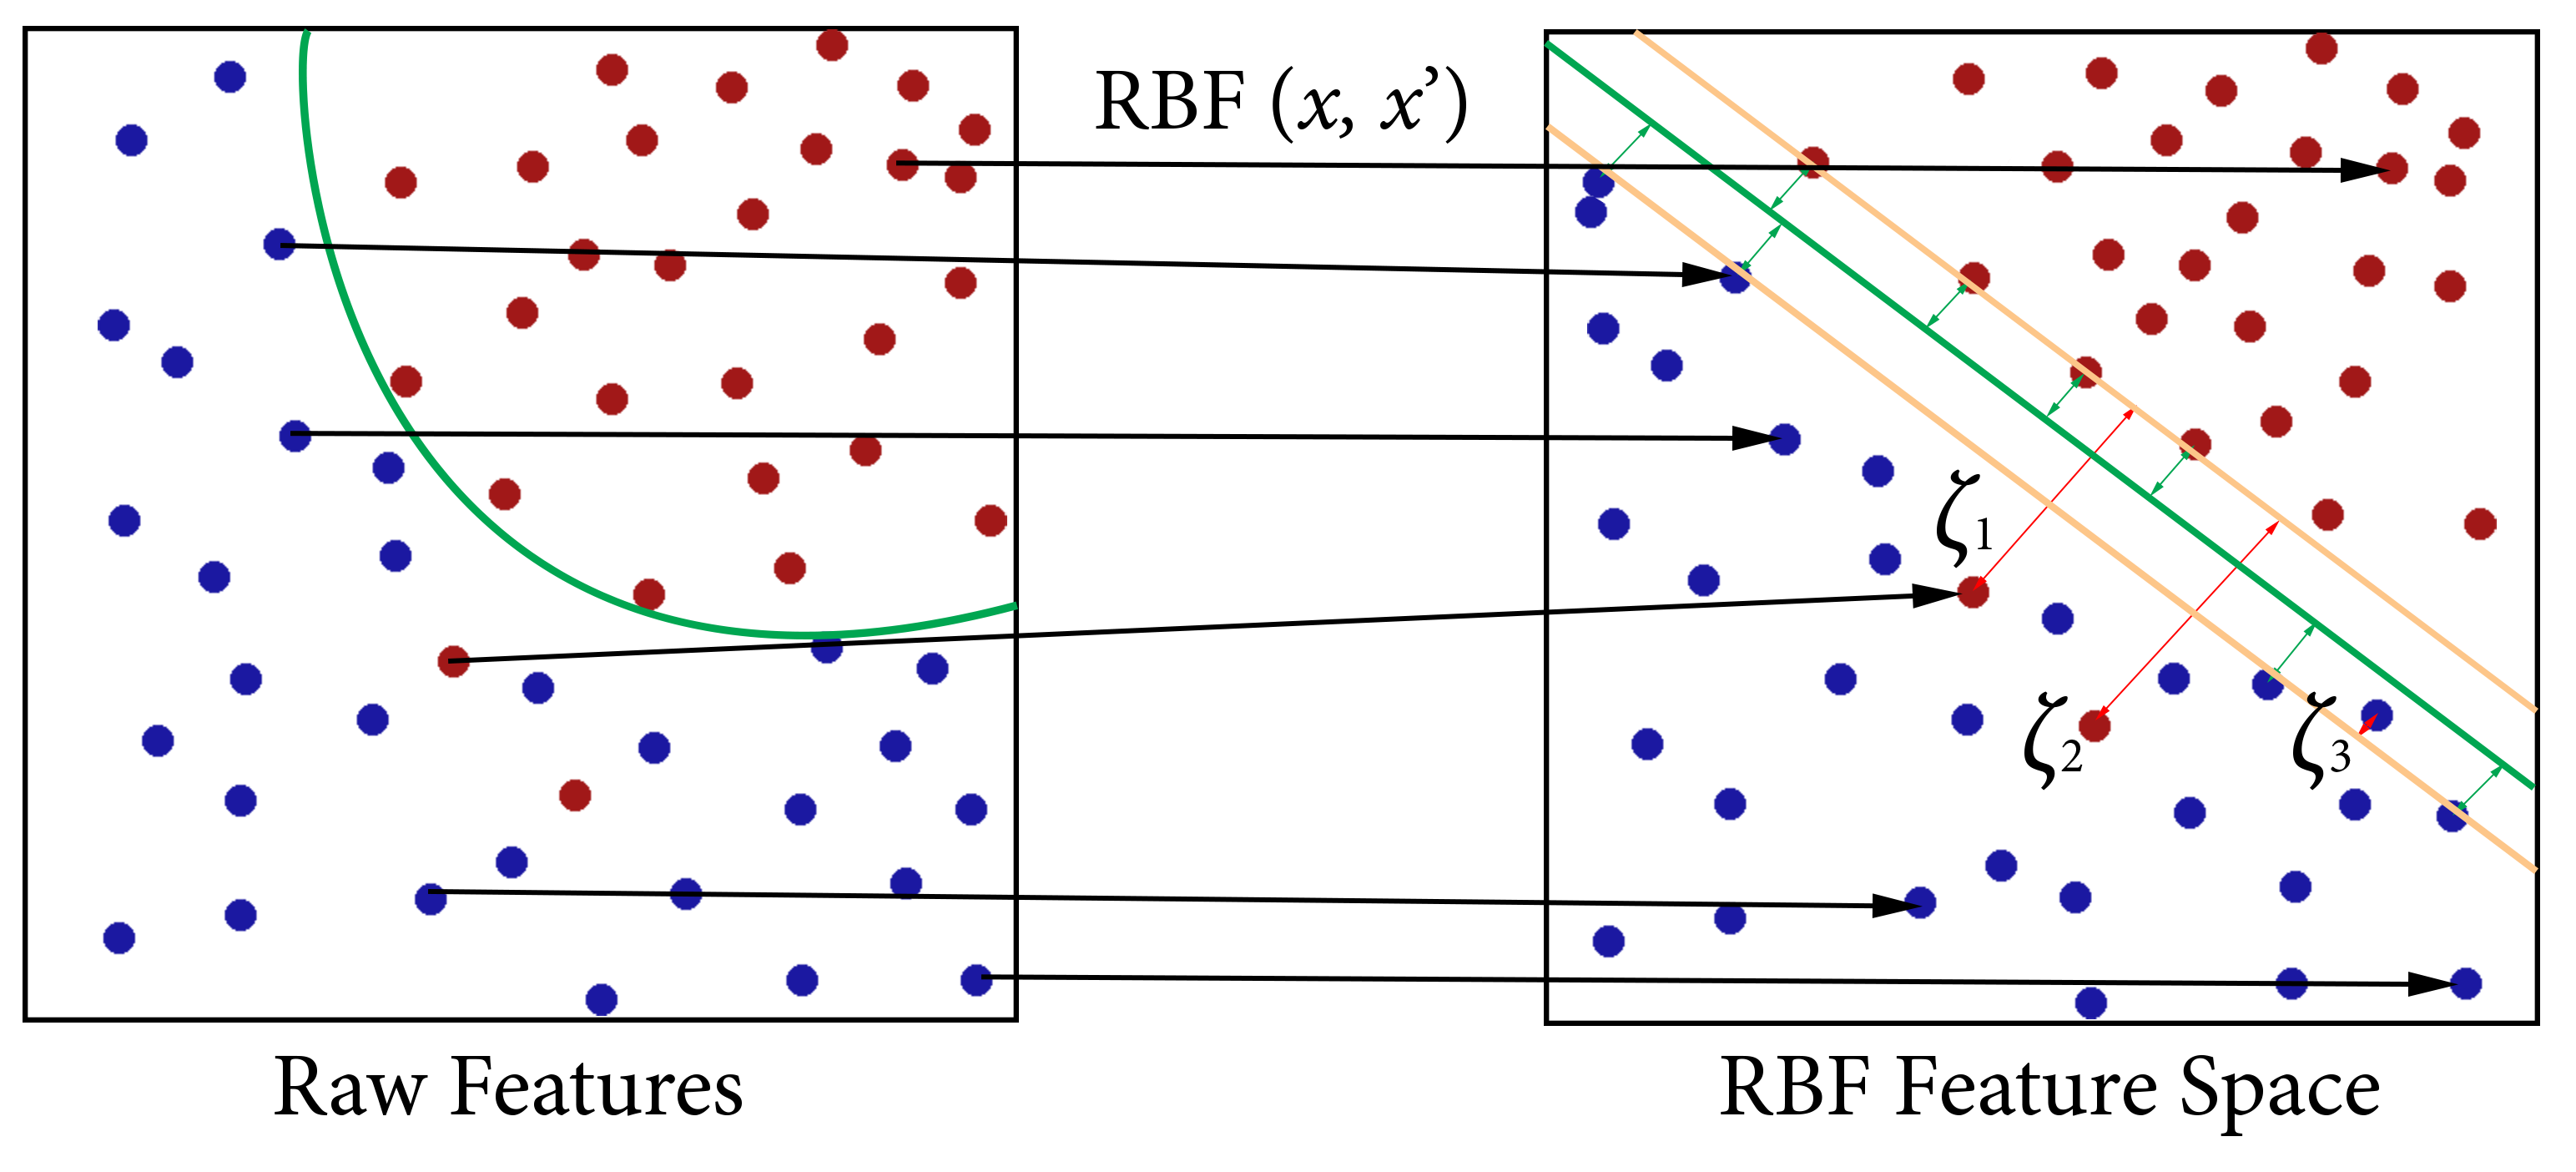
\includegraphics[width=0.8\linewidth]{svm.png}
	\caption{A RBF kernel is used to transform the data into a more linearly separable space. $\zeta_i$ denote slack variables which lie beyond the margin (depicted by beige lines). }
\end{figure}

The original SVM algorithm was not able to handle cases where data was not separable. Cortes and Vapnik~(1995)~\cite{svmsoftmargin} introduced slack variables $\zeta_i$, which define a penalty for data beyond the SVMs margins thus extending the use of SVMs to non-separable data. The sum of these slack variables is added to the SVM's Lagrangian equation along with a constant scaling factor $C$. The parameter $C$ balances the penalty for data beyond the margins with the size of the margin. A small $C$ is incentive to create a large margin whereas a large $C$ is incentive to minimize errors.

The combination of kernels and slack variables greatly improved the applicability of SVMs. SVMs became very popular in the machine learning community as they were simultaneously analysable and powerful. However, kernels and slack variables also introduce a number of hyperparameters, such as the scaling factor $C$ and the type of kernel and its parameters. Although intuition and knowledge of the data can guide kernel and hyperparameter choice, techniques such as grid or random search~\cite{gridsearch} are generally used to fine-tune them. However, hyperparameter tuning increases the risk of overfitting, which will be discussed in detail in section~\ref{detectoverfit}. 


\subsection{Artificial Neural Networks}
%Most traditional machine learning models are derived under the assumption of independent and identically distributed data. The

%Random forests and SVMs are 
 
Traditional machine learning models perform best when data is structurally simple. Most statistical models such are designed to fit a linear function through the data, using pre-defined basis functions or the kernel trick to reduce non-linearity. Random forests and decision trees are powerful when data is readily available, however they do not model functions of data and are less suitable when predicting unseen outliers~\cite{kramer2001propositionalization}. Neural networks are popular models used when the dataset is reasonably sized and there exists a difficult to describe structure in the input features. They are extremely powerful, however very difficult to interpret or debug and highly prone to overfitting.
 
\label{neuralnetworkintro}Although neural networks have only recently risen to the spotlight, their history begins in 1943 with the introduction of a computational model of biological neurons\footnote{\emph{Neurons} are cells which transmit information via chemical and electrical signals. They are the fundamental building block of the human brain.}~\cite{nn1943}.
In 1958, the simple perceptron learning algorithm was developed~\cite{rosenblatt1958perceptron}, which would become the building blocks of neural networks today. The fundamental concept of a neural network is connecting many perceptrons (acting as neurons) together to simulate the behaviour of a biological brain. 




\begin{figure}[h]
\label{perceptron}
\centering\includegraphics[width=1\linewidth]{perceptron.png}
\caption{The simple perceptron learning algorithm. The original incarnation could not handle inseparable data~\cite{rosenblatt1958perceptron}. Images borrowed and modified from Bishop~(2006)~\cite{prml} }
\end{figure}

A perceptron by itself is a simple machine learning model, taking input features  and outputting a value representing a class or probability. As neurons were thought to have two states --- either firing or not --- the output was passed through a Heaviside\footnote{A discontinuous function which outputs either 0 or 1, defined as $ H(x)=\begin{cases} 
      0 & x < 0 \\
      1 & x \geq 0 
   \end{cases}
$} \emph{activation function}. At the time, computational power was limited and large networks impossible to train. Early works by Minsky and Papert~(1969)~\cite{minsky1969perceptrons} were misinterpreted as stating that perceptrons were incapable of modelling the `exclusive or' (XOR) function. However Minsky and Pampert only proved this for a single perceptron and believed that multiple layers of perceptrons could model the XOR function. In 1989, it was shown that a single layer with enough perceptons is able to approximate any non-linear continuous function~\cite{nnuniversalapprox}.


\begin{figure}[h]
\label{perceptronvis}
\centering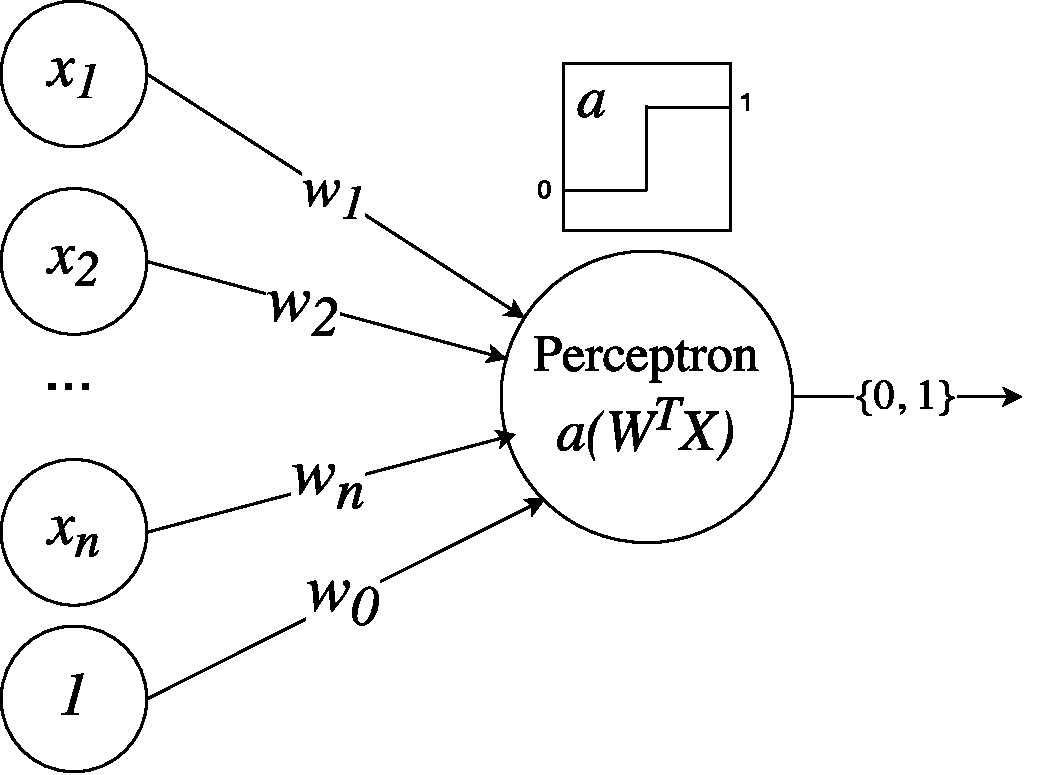
\includegraphics[width=0.5\linewidth]{perceptron.pdf}
\caption{A single perceptron node. Takes input $X$ and learns the weight vector $W$ to classify the output with the Heaviside activation function $a$.}
\end{figure}

Although multiple layers of perceptrons had always been the goal of neural network research, training them was not possible until backpropagation, a form of gradient descent\footnote{Surprisingly, Werbos' work on backpropagation~\cite{werbos1974beyond}  was lost and would be rediscovered a decade later in 1985 by Rumelhart et~al.~\cite{backproprediscover}} was introduced~\cite{werbos1974beyond}. Backpropagation required the activation function to be differentiable, hence the sigmoid\footnote{The sigmoid function is defined as $\sigma(n) = \frac{1}{1+e^{-x}}$}  replaced the Heaviside activation function. Neural networks were now able to reliably `learn' complex non-linear functions, although computational power would be a bottleneck for a couple of decades. \textit{Deep learning} or \textit{Deep neural networks} are a general term for neural networks with many (generally more than 3) layers.

%. Unlike SVMs, a kernel does not have to be predefined - a neural network is able to learn a non-linear function of the data.

\begin{highlight}
A neural network's ability to learn complex non-linear relationships provides a significant advantage over traditional models where this non-linearity must be pre-defined.
\end{highlight}

\begin{figure}[h]
\label{nnetstacked}
\centering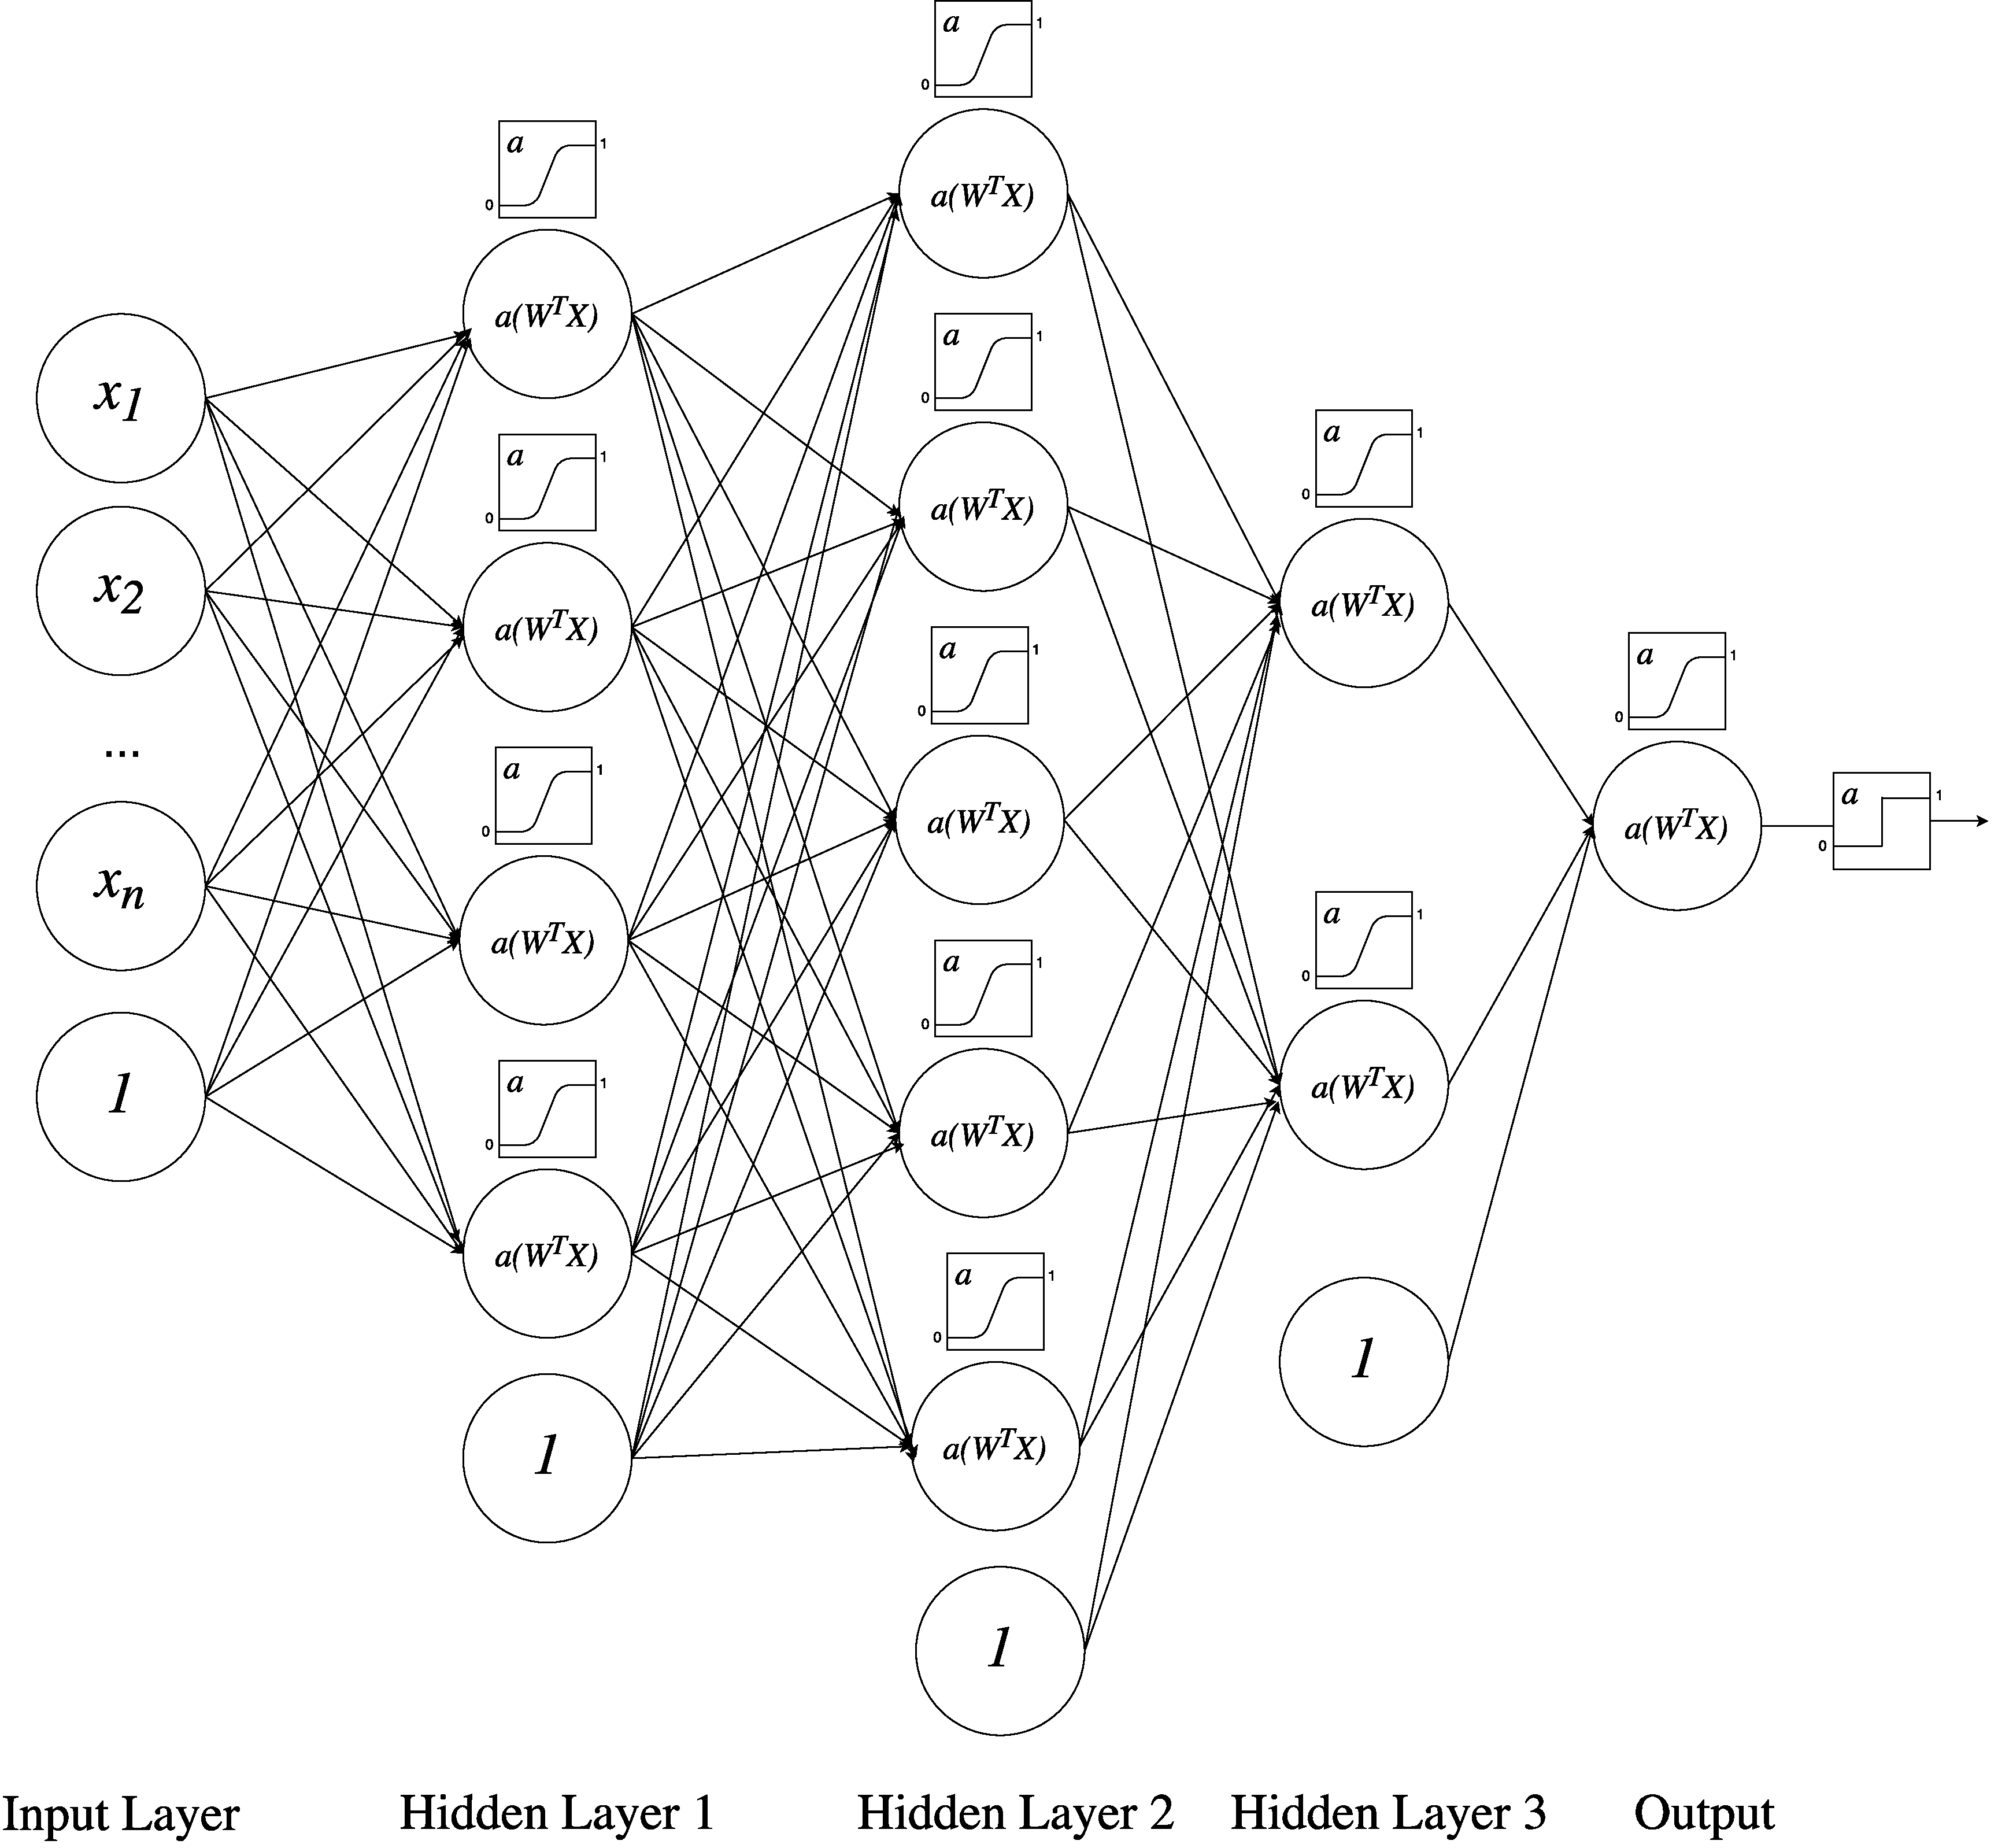
\includegraphics[width=1\linewidth]{neuralnet.pdf}
\caption{A simple 3 hidden layer fully connected neural network with sigmoidal activations. By stacking non-linear activation functions, neural networks are able to learn any non-linear function of the input. The '1' nodes represent the bias at each layer.}
\end{figure}


Neural networks are computationally expensive models and unlike traditional models, training requires optimising a non-convex function. This is computationally intractable and current neural networks are trained by finding a good local optima through gradient descent with backpropagation~\cite{convexopt}. The vanishing gradient problem~\cite{vanishinggradient} limited the depth of neural networks until the recent development of batch normalisation~\cite{batchnorm}. Previously, careful management of gradient flow was required to train deep neural networks~\cite{googlenet}. 

Two major variations of the traditional fully connected structure are convolutional and recurrent neural networks. Convolutional neural networks (\emph{CNNs}) are inspired visual cortex, where neurons are connected to local regions of the visual field. These networks contain `convolution' layers where neurons are connected to a small local region of neurons in the previous layer. These convolution layers learn a hierarchy of `features' and can negate the need for feature extraction for certain types of input data. This is especially evident in the task of image recognition, where CNNs have rapidly exceeded the performance of traditional models.


\begin{figure}[h]
	\label{cnnvis}
	\centering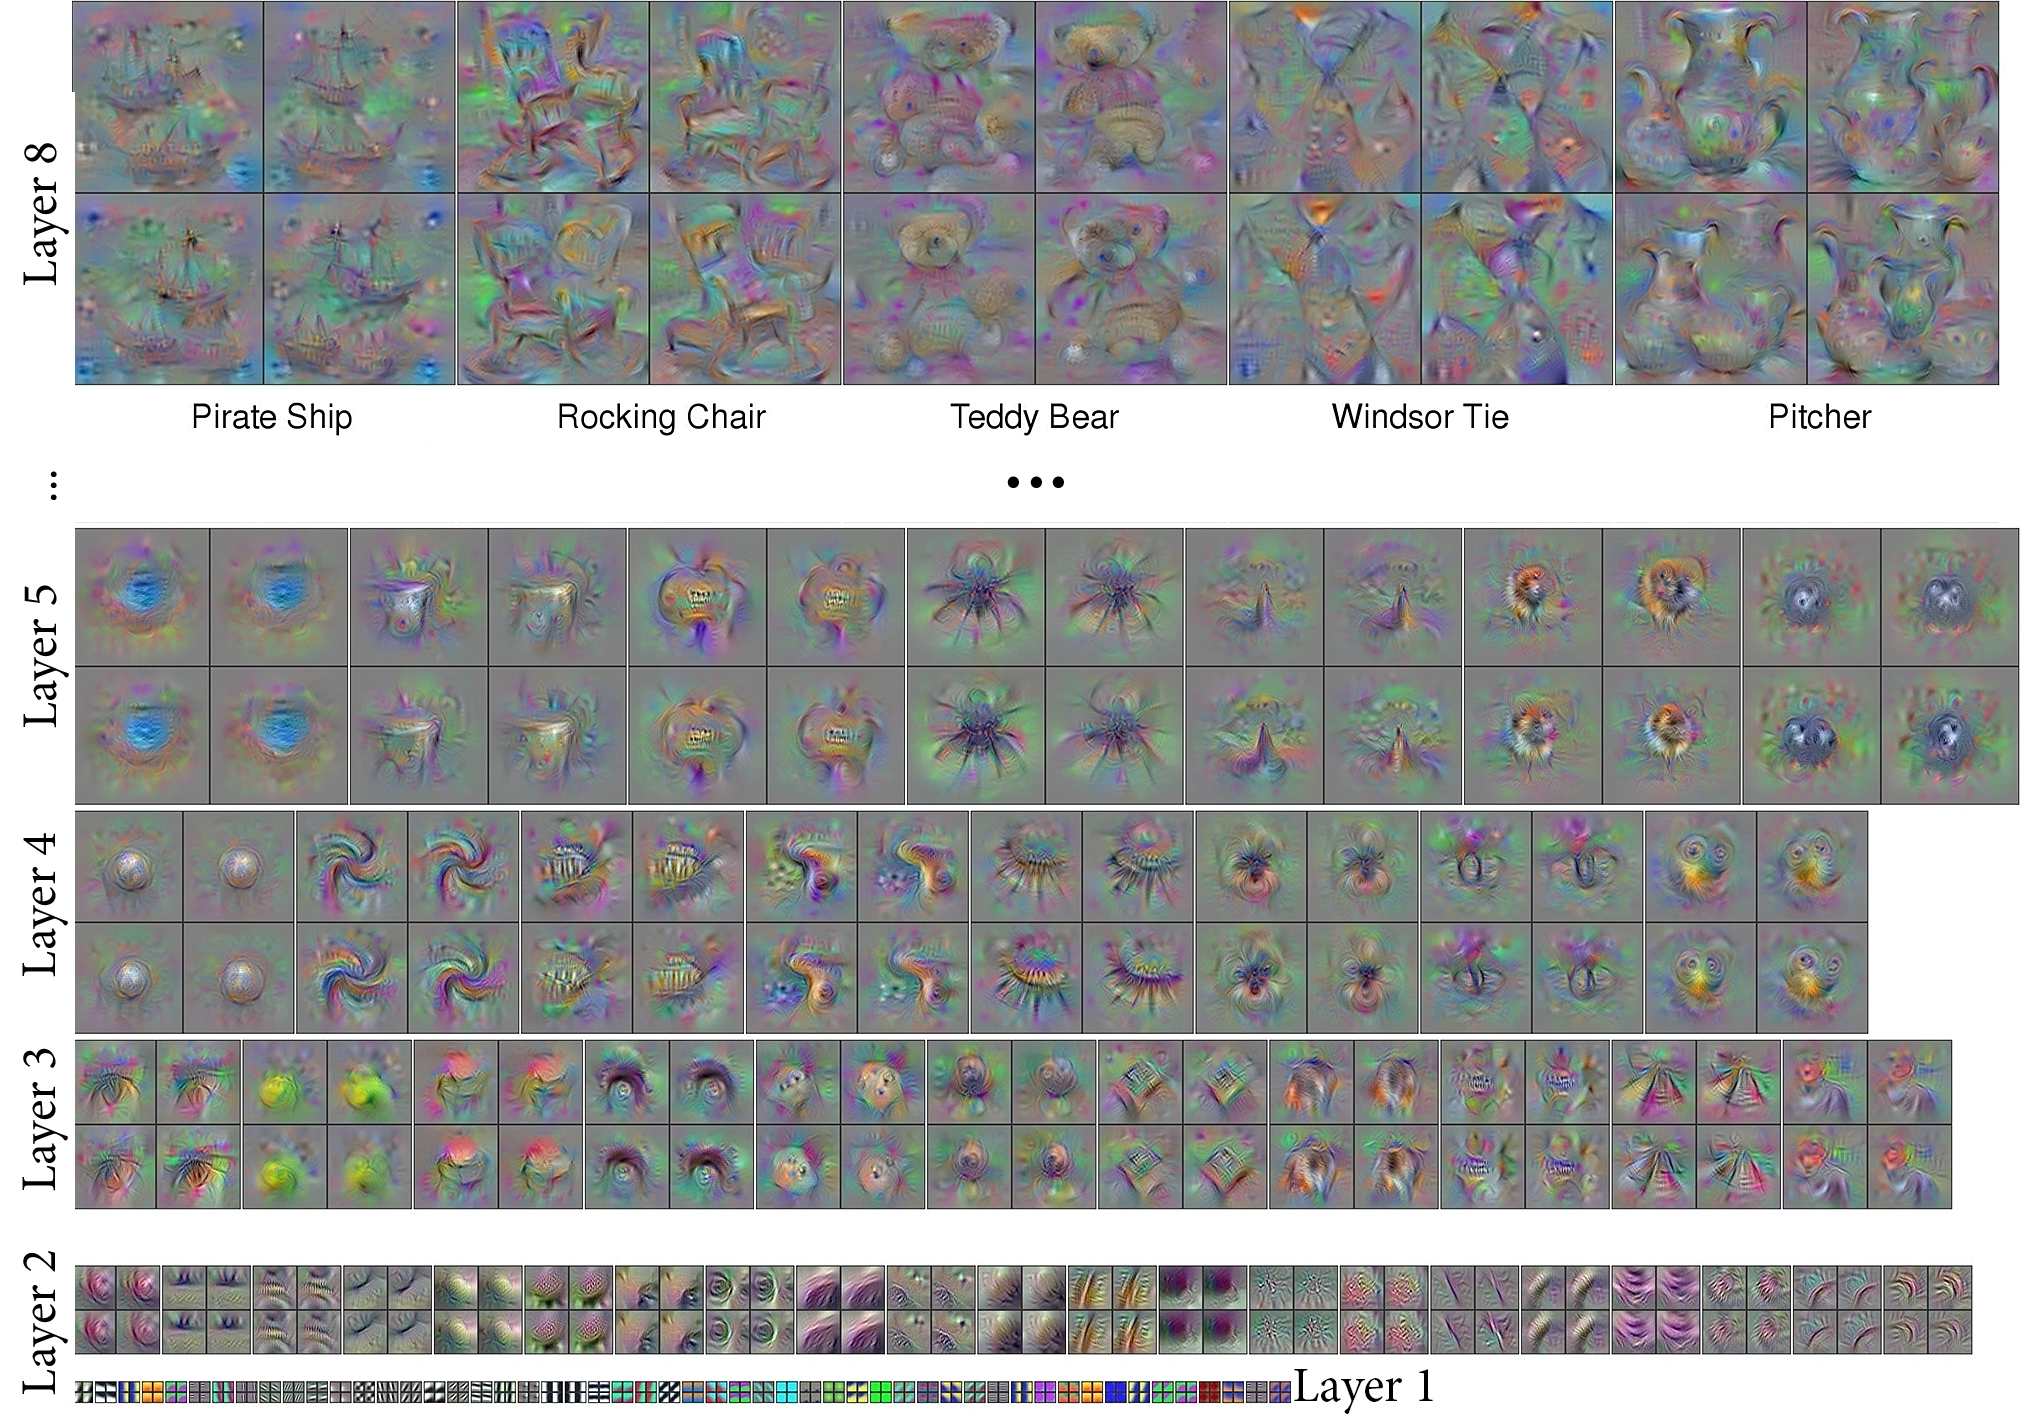
\includegraphics[width=1\linewidth]{cnnvis.png}
	\caption{A visualisation of CNN nodes from Yosinski et al.~\cite{cnnvis}. Layers capture increasingly complex relationships between pixels and act as features input into further layers. }
\end{figure}


Recurrent neural networks (\emph{RNNs}) are neural networks with cyclic connections. This essentially creates an internal state which allows neural networks to better handle temporal data and provides flexibility for the type of input and output data. There are a number of RNN variants, however long short-term memory (LSTM) nodes are applied in practice as they are more robust to the vanishing gradient problem~\cite{lstm}. A recent model combining LSTM and convolution layers has been very effective at classifying visualised EEG data~\cite{bashivan2015learning}.


\subsubsection{Neural Network Hyperparameters}
Neural networks inherently have a large number of hyperparameters. This section will provide a basic intuition behind selecting hyperparameters of a neural network. 

The most fundamental features are the width and depth of the network. In general, increasing the number of nodes in a network reduces it's bias and is more suitable when the structure of data is complex or data is plentiful. It is thought that networks with many nodes per layer (\emph{width}) are better at memorization whereas additional layers (\emph{depth}) are better at generalisation of features~\cite{cheng2016wide}. Depth can also be exponentially more valuable than width for modelling the structure of complex non-linear data~\cite{eldan2016power}. There is still no consensus on the balance between number of nodes and layers --- these must be fine tuned for particular problems with intuition and search.

A large neural network has a tendency to overfit by memorising the data. Regularisation is a method of preventing this without reducing the size of the network. In traditional machine learning, $l_1$ and $l_2$ weight regularisation is most common. This involves adding a penalty to weights, motivated by Occam's razor where a simpler model is preferred. However in the context of neural networks, weight regularisation slows convergence and complex models can still be learned with a deep enough network. {Early stopping} and {dropout} are the most common forms of regularisation in practice. 

\emph{Early stopping} involves stopping training before the optima is reached, at the point where the cross-validation accuracy starts to decrease from overfitting. \emph{Dropout} involves randomly disabling some percentage of nodes on each layer at each iteration of gradient descent~\cite{dropout}. At first, this may appear unintuitive, however the idea is to promote redundant feature representations to improve its robustness. Dropout generally outperforms weight regularisation, and a combination of dropout and early stopping is commonly applied. There are also variations of dropout such as dropconnect~\cite{dropconnect} where connnections rather than nodes are zeroed.

A major problem with the sigmoidal activation function is that as the activation approaches either 0 or 1 the gradient approaches zero. This is known as \textit{saturation} and significantly slows the convergence of gradient descent in the training process. Rectified linear units (\emph{ReLUs}) use the activation function $f(x) = \max(0,x)$ which resolve the gradient issue and are believed to be more biologically plausible~\cite{relu,relubiology}. One notable characteristic of ReLUs is that once the unit outputs zero, it is essentially `dead' as the gradient of the rectifier is zero. A number of modifications to ReLU have been proposed such as the leaky/parametric ReLU~\cite{he2015delving} ($f(x) = \max(\alpha x, x)$ for $\alpha\leq 1$), Maxout~\cite{goodfellow2013maxout}, noisy ReLU~\cite{noisyrelu} and exponential linear unit~\cite{clevert2015fast}.

The initialisation of the weights in the network will affect the solution found by gradient descent and the rate of convergence to it. Poor initialisation can result in the death of ReLUs or saturation of sigmoidal and tanh units. Glorot and Bengio~\cite{glorot2010understanding} proposed initializing the weights according to a Gaussian distribution with variance $2/(n_{\text{in}}+n_{\text{out}})$ where $n_{in}$ is the number of inputs to the node and $n_{out}$ the number of outputs. This is commonly termed Xavier initialisation and is effective for networks with sigmoidal or tanh activations however ReLUs rapidly tend to zero. He et~al.~\cite{he2015delving} proposed a small modification to fix the dead ReLU issue by setting variance to $2/n_{\text{in}}$.

The method of gradient descent, referred to as the \textit{optimizer} is also a major area of neural network research. Traditional gradient descent often gets stuck at saddle points and local minima as the gradient is zero. Non-linear techniques developed in convex optimisation such as conjugate gradient descent and (Quasi-)Newton are powerful yet rarely applied in practice due to their computational complexity. The most popular optimizers for neural networks incorporate the concept of momentum, where previous gradients are considered in the descent. Adam~\cite{adam} is one of the most recent optimizers and combines elements from two powerful optimizers before it, AdaGrad and RMSProp. Nesterov momentum~\cite{nesterov1983method} --- which has favourable properties in convex optimisation --- can also be incorporated into Adam, creating Nadam.~\cite{nadam}. 

\begin{figure}[h]
	\label{cnnvis}
	\centering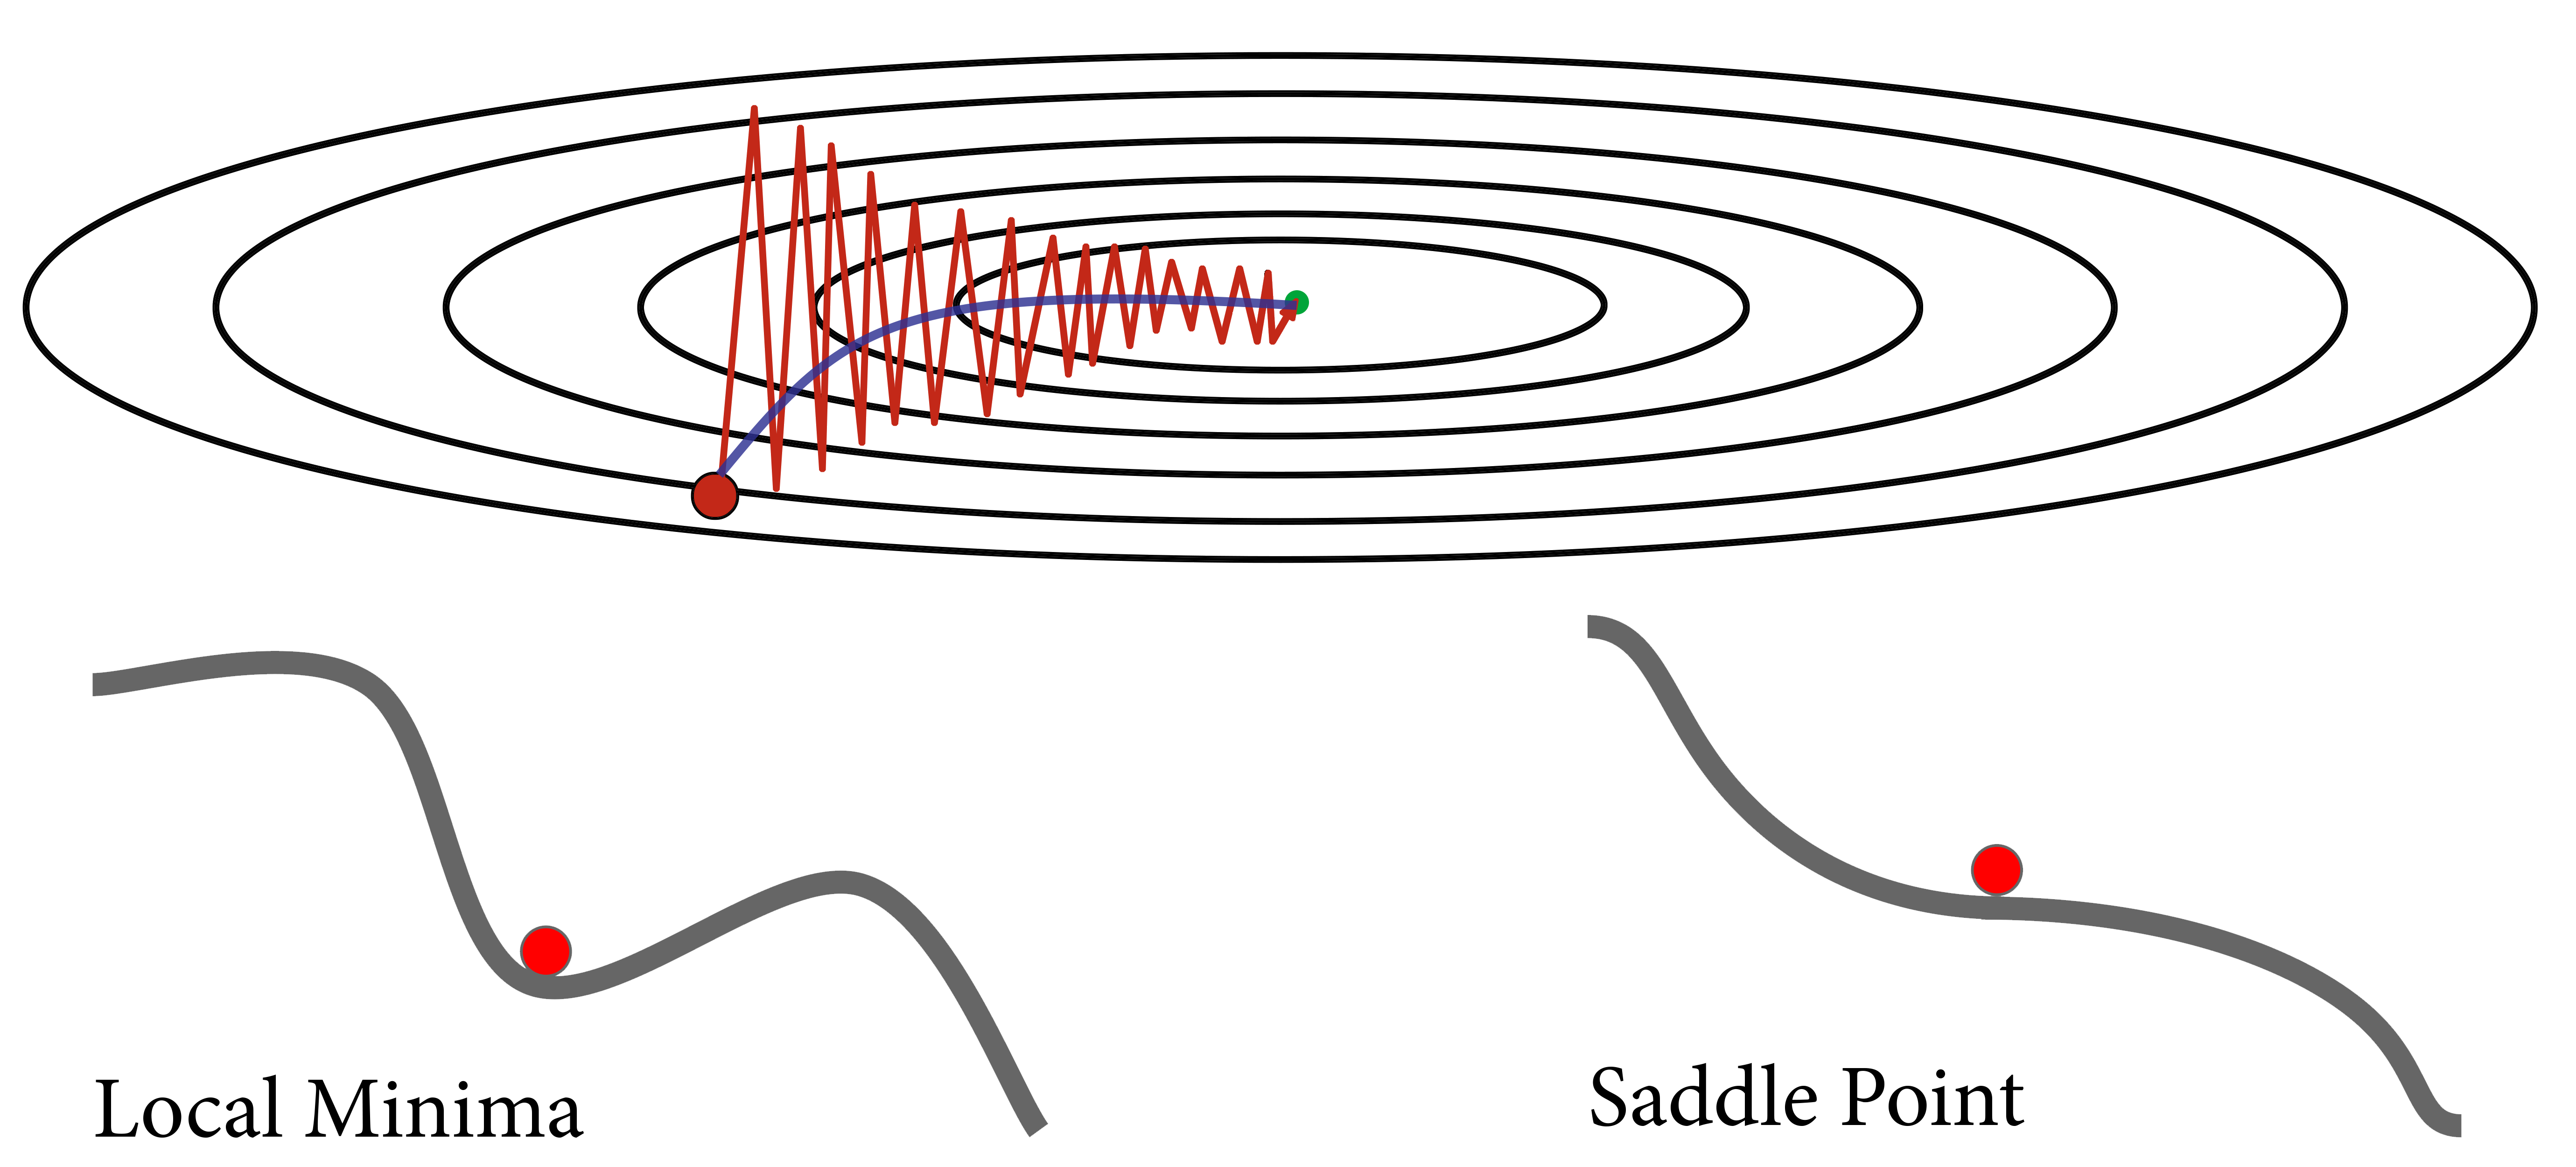
\includegraphics[width=0.82\linewidth]{gradescent.png}
	\caption{Traditional gradient descent (red curve) performs poorly in `long valleys'. Optimizers generally use momentum to simulate the behaviour of the optimal blue curve and avoid local minima. Diagram adapted from Stanford's CS231n~\cite{cs231n}.}
\end{figure}

Each optimizer also has its own hyperparameters, the most major one being the learning rate. As training is stochastic, training multiple models and using them in an ensemble often results in better performance. Loshchilov and Hutter (2016) have proposed a novel approach where the learning rate is fluctuated during training to create an ensemble in one training process~\cite{sgdrestarts}. 


\subsection{Feature Selection and Dimensionality Reduction}
The general approach to a machine learning problem is to extract as many features as possible then determine which are most relevant\footnote{There are issues with this approach such as Freedman's paradox~\cite{freedmanparadox} however resolving this is the task of model evaluation (section \ref{detectoverfit}).}. Redundant or highly correlated features reduces the performance of most machine learning algorithms. Simple models like Naive Bayes rely on the assumption that features are independent and correlated features can disproportionately weigh certain factors. Neural networks are better equipped to handle correlated and redundant features, however may require more data or training time to do so. 


\begin{highlight}
	Feature selection techniques aim to eliminate useless features and dimensionality reduction reduces the correlation between features.
\end{highlight} 

\emph{Feature selection} simplifies the model by selecting a subset of features to use. This increases the interpretability of a model, reduces the probability of cross-validation overfitting~\cite{overfittingcv} and speeds up training. Selecting an optimal subset of features is not a simple task as some features may be uninformative on its own but useful when combined with others. An exhaustive search would be required to determine the optimal subset however is computationally infeasible. Feature selection algorithms aim to quickly find a good subset and can be categorised as filters, wrappers and embedded methods. 

\emph{Filters} evaluate subsets of features by maximising various criteria such as entropy, similarity and other statistical measures. Evaluation of subsets is generally fast and results are independent of machine learning model. However a majority of filters are based on the assumption of linearity and may not be suitable when complex relationships exist between features. \emph{Wrappers} `wrap' around existing models, using cross-validation to evaluate a feature subset. This allows the selected features to be better tailored to each model. However wrappers can be computationally prohibitive when wrapping around models such as neural networks and also cater towards the model's tendency to overfit~\cite{wrapperoverfit}. \emph{Embedded} methods rely on machine learning models which inherently perform feature selection during their training, often from strong regularisation. 

The performance of these approaches are highly problem-dependent. This thesis will employ a number of state of the art supervised feature selection algorithms as depicted in table \ref{featureselection}.  We refer to Li~et~al.~\cite{skfeature} for a thorough description and comparison of these techniques. 

\begin{table}[h]
	\caption{Feature selection methods used in this thesis. Neural network forward/backwards search was not performed as resources were limited.}
	
	\label{featureselection}
	\centering
	\begin{tabular}[t]{c c c}
		\toprule
		{\specialcellbold{Filter}} &
		{\specialcellbold{Wrapper}} &
		{\specialcellbold{Embedded}}\\
		\midrule
		
		\begin{tabular}[t]{@{}l@{}}ReliefF~\cite{relieff}\\ 
		Fisher score~\cite{fisherscore}\\
		CIFE~\cite{cife}\\
		JMI~\cite{cife}\\
		ICAP~\cite{icap}\\
		MIFS~\cite{mifs}\\
		MRMR~\cite{mrmr}\\
		CFS~\cite{CFS}	
		\end{tabular}
		& 
		
		\begin{tabular}[t]{@{}l@{}}SVM/Gaussian Process\\
			Forward/Backwards\\
			Search
		\end{tabular}
		&
		\begin{tabular}[t]{@{}l@{}}RFS~\cite{rfs}\\
			ls\_l21~\cite{l21}
		\end{tabular}	
		\\
		\bottomrule
	\end{tabular}
\end{table}

Rather than eliminating features, \emph{dimensionality reduction} aims to reduce the amount of information required to represent the set of features. This reduces the correlation between features and can significantly improve performance with simpler models. The two most common forms of dimensionality reduction are the unsupervised principal component analysis (PCA) and supervised linear discriminant analysis (LDA) and variations~\cite{prml}. Neural networks can also be used to reduce the dimensionality of data by training a network to predict the input where the center hidden layer contains fewer nodes than the input. These are termed autoencoder networks and can out-perform PCA however are difficult to analyse~\cite{nndimred}.	 


\begin{highlight}
Feature selection is almost a requirement for small datasets, whereas dimensionality reduction is less commonly applied as it can obfuscate the model. 
\end{highlight}

\subsection{Model Evaluation and Handling Overfitting}
\label{detectoverfit}
The primary goal of machine learning is to train a model which will generalize well to new data. Accuracy over the entire dataset is evidently not a good metric, as an model which memorises the data (overfit) can appear to have perfect accuracy while failing to generalize to new data. Model selection and evaluation is the field in statistics which handles this. However the field is contentious --- especially as model selection performance varies based on the type of data. 

Cross validation (\emph{CV}) has become the de-facto standard in machine learning. Conceptually, CV is very simple. The primary types used in machine learning are \textit{leave one out} and \textit{k-fold}. Lets assume there are 100 data points in a dataset. In leave one out CV (LOO), 99 data points are used to train a model, and 1 data point to test and evaluate the performance. This is repeated over each  data point and the average result taken as the generalization accuracy. K-fold is similar, however rather than using only one data point, the data is split into $k$ groups, training on $k-1$ and testing on $1$ group. For example, 2 fold CV involves training on fold 1 and testing on fold 2 then training on fold 2 and testing on fold 1. Common values of $k$ are 2, 5 and 10.   

In summary, we will be performing 10 fold cross-validation with random stratification\footnote{\emph{Stratification} involves ensuring there are an equal number of classes in each set. In this case, people with and without PD. } repeated 10 times. This results in a set of 100 accuracy values after taking the mean accuracy of each fold of cv for each model. The same stratification sets are used, and Bayes factor~\cite{bayesianttests} is used to test if the mean performance of one model is greater than the other. This decision will be justified in the next section with more background into model selection and hypothesis testing provided.

\subsubsection{Model Selection and Hypothesis Testing}
\label{msht}
K-fold and LOO CV are the de-facto standards in machine learning, and it is rare to look for alternatives. They provide a good estimate for generalisation error, are easy to implement and fast to evaluate. Leave one out CV allows almost all the data to be used in training. When the data is clean (high signal to noise ratio) LOO performs nearly unbiased estimations~\cite{crossvalsurvey}. However LOO has been criticized for preferring models with a high variance and is less computationally feasible for large data sets~\cite{kohavi1995study}. Kohavi~(1995)~\cite{kohavi1995study} instead recommends 10 fold CV in the general case. CV variations such as exhaustive and Monte-Carlo CV exist however they are not recommended by statistical literature~\cite{kfoldvsloo, crossvalsurvey}. 

There are a number of catches when performing CV:
\begin{itemize}
	\item CV requires validation data to be independent from training data. In medical contexts it is common to have multiple recordings from a single patient. Recordings from the same patient are likely to share similar attributes and cross-validating naively over the whole dataset can easily overfit.
	\item When performing hyperparameter optimisation the CV score is often used as a metric. The risk that the best model fits the validation sets well by pure chance increases as more parameters are explored~\cite{overfittingcv}.
\end{itemize}

Overfitting cross-validation is difficult to detect without additional data and is a major issue in small datasets. A common approach is to take a subset of data as the `test' data which remains unseen in hyperparameter optimisation, however this is infeasible when there is not enough data to create a test set large enough for results to be meaningful. Ng~(1997)~\cite{overfittingcv} proposes an algorithm to select from a number of competing hypothesis. Repeating k-fold CV with different division of folds can also reduce the likelihood of models overfitting CV by chance. Bouckaert~(2003)~\cite{bestcvempirical} recommends 10 fold CV repeated 10 times after extensive empirical testing.

Accuracy is the most basic and intuitive measure of performance, however it has been the subject of a number of criticisms. Firstly, it is susceptible to the false positive paradox\footnote{The false positive paradox occurs when there is a very low incidence of a positive results in the target population. For example, when only 1\% of the population suffer from PD, a model which only predicts `no PD' will be completely uninformative yet perform better than any model which predicts PD sometimes.} and may not be a good representation of a model's effectiveness in difficult tasks. Sensitivity, or true positive rate is a measure of the percentage of positive classes correctly identified and specificity or true negative rate measures the percentage of correctly identified negative examples. The \emph{$F_1$ score} is the harmonic mean of sensitivity and specificity and is an effective measure of model performance when classes are unbalanced. 

Secondly, accuracy does not take into consideration the confidence of a model's predictions. The area under the ROC (Receiver Operating Characteristics~\cite{rocauc}) curve (\emph{AUC}) was proposed as a better alternative to accuracy. The ROC curve is created by plotting sensitivity and specificity at all confidence thresholds and the area under ROC was believed to be a more robust and statistically consistent measure of model performance~\cite{aucgood}. However recent empirical experiments have shown that AUC favours particular models~\cite{aucmislead2} and it has been criticised for being incoherent~\cite{aucmislead, aucincoherent}. Modifications to AUC have been proposed~\cite{aucmislead2, aucincoherent} however they are uncommon in practice. As a result, accuracy and $F_1$ score will be the primary performance measures utilised in this thesis as they are interpretable and model characteristic independent.


Hypothesis tests are used to determine if the results obtained in experiments are \textit{statistically significant}. After obtaining the accuracies or $F_1$ scores for each fold of cross validation, a hypothesis test should be used to determine that the difference in results is not from chance. A paired t-test is the traditional approach to testing if one population mean is greater than another. There have been criticisms of frequentist hypothesis testing promoting the publication bias~\cite{publicationbias}, citing the non-replicability crisis in psychology~\cite{replicability}. Recently, the American Statistical Association has officially endorsed Bayes factor~\cite{bayesianttests} as their preferred method of hypothesis testing~\cite{bayesfactorASA}, and mass-replication studies have shown that almost half of previous psychological research do not meet the criteria for strong evidence when Bayes factor is applied~\cite{bayesfactorempirical}. The standard two tailed Cauchy distribution is used as a prior in this thesis~\cite{bayesianttests}.


In statistics, there is no agreed upon method for model selection and evaluation. Penalization based evaluation\footnote{\emph{Penalization} based model criteria are inspired by Occam's razor, preferring simple model over a more complex one which obtains similar results as it is less likely to overfit}  criteria such as Akaline/Bayesian/General Information Criterion~\cite{aicbic,generalinfocriteriongic} and Minimum Description Length~\cite{mindescriptionlength} are common model selection techniques. However these are less suitable for machine learning as it is difficult to quantify the complexity of model such as neural networks. Cross validation is therefore the only feasible technique to compare completely different models. 
 



%Dieterrich recommends two fold, understimate variance ~\cite{bestcvapproximate}
%\cite{nounbiasedkfoldcv}




\chapter{Our Work}
\label{ourwork}
Although there is a rich selection of prior work in PD diagnosis with machine learning, the lack of a standard dataset and methods limits the comparability of different studies. There have been two large scale literature reviews, Alhrics et~al.~(2013)~\cite{review2013} and Bind et~al.~(2015)~\cite{review2015}. In these reviews it is apparent that multiple sub-fields exist and research is often confined in its own sub-field. For example, the top papers in the Interspeech 2015 PD speech challenge~\cite{compareis15pd} used methods independent of the dysphonia feature extraction previously done for PD. Research also rarely considers the results of works completed in challenges such Interspeech or Michael J. Fox Foundation Parkinson's data challenges~\cite{mjfoxchallenge2013}. It is common to find a paper failing to cite prior work which performs the same experiments. A goal of this thesis is to consolidate and distil prior work into a easily digestible format. 

\begin{highlight}
Multiple sub-fields exist in PD literature and research is often isolated within a sub-field.
\end{highlight}

Although prior works have reported good results, it is difficult to determine if these results are caused by biases in the dataset or overfitting. With any field based on empirical statistics, a publication bias exists~\cite{publicationbias} and there will exist results which are not replicable~\cite{replicability}. Section \ref{detectoverfit} details measures to avoid overfitting and evaluate models however their implementation is uncommon in applied machine learning literature. The variation of results on experiments with very similar setups shines doubt on the replicability of results for some of the best performing papers. Arora~et~al.~(2014)~\cite{arora2014high} achieves 98.0\% accuracy using smartphone IMU data from 20 participants. Zhan~et~al.~(2016)~\cite{zhan2016high} performs an experiment using all features in Arora~et~al.~(2014) as well as additional speech and tapping measures however only manages 71\% accuracy. Furthermore, the state of the in motion mode recognition rarely achieves such results despite the motion mode recognition likely being the `easier' task~\cite{motionmoderecognition}.

The following sections detail the experiments performed as part of the project. We will apply a combination techniques used in state of the art on a larger dataset to assess true performance. The mPower dataset~\cite{mpower} has been chosen for this  task and will be described in the following section.

%Although each section may be read independently, reading sequentially is recommended as later sections may reference conclusions of prior ones.
\begin{itemize}
\item Section \ref{mpower} discusses the dataset used (mPower) and how the data was filtered and pre-processed.
\item Section ....
\end{itemize}

\section{The mPower Dataset}
\label{mpower}
To minimize the likelihood of bias or overfitting, a larger dataset was required. Currently, the only publicly available dataset that satisfies the size requirements is mPower~\cite{mpower}. 

\begin{figure}[h]
\label{mpowerapp}
\centering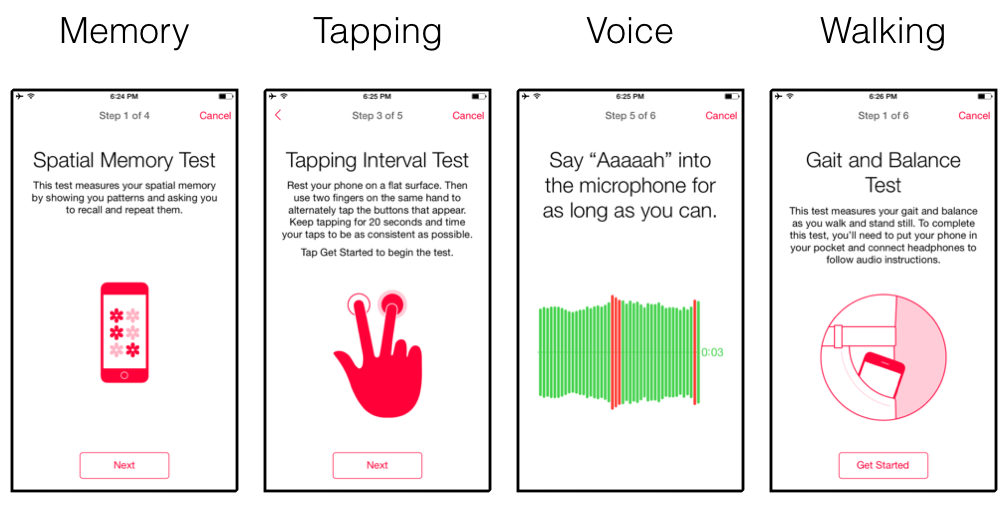
\includegraphics[width=1\linewidth]{mpower.png}
\caption{The mPower app consists of several tasks to evaluate memory, bradykinesia, voice and gait. }
\end{figure}

The mPower study began in March 2015, open to people living in the United States who owned an Apple iPhone or iPod released in 2011 or later. Upon downloading the app, the user was presented with the tasks presented in figure \ref{mpower} along with general demographics questions and UPDRS questions. Each task/questionnaire was optional and could be completed multiple times. As of writing, there are around 6,500 participants in the study, 1,100 with PD. Users come from a variety of backgrounds and may have other illnesses (however this was not recorded as part of the dataset).

The mPower dataset also contains a number of cases of young-onset Parkinson's disease\footnote{Assuming the participants are honest of their circumstances.}~\cite{youngpd1, youngpd2} which has rarely been studied in a diagnosis context. Age is a bias in the dataset as a majority of the non-PD participants in the study were young adults. Using age alone, the prediction PD $\Leftrightarrow$ age $> 52$ would result in 86.1\% accuracy.

\addtocounter{footnote}{-1}
\begin{figure}[h]
\label{overfitex}
\centering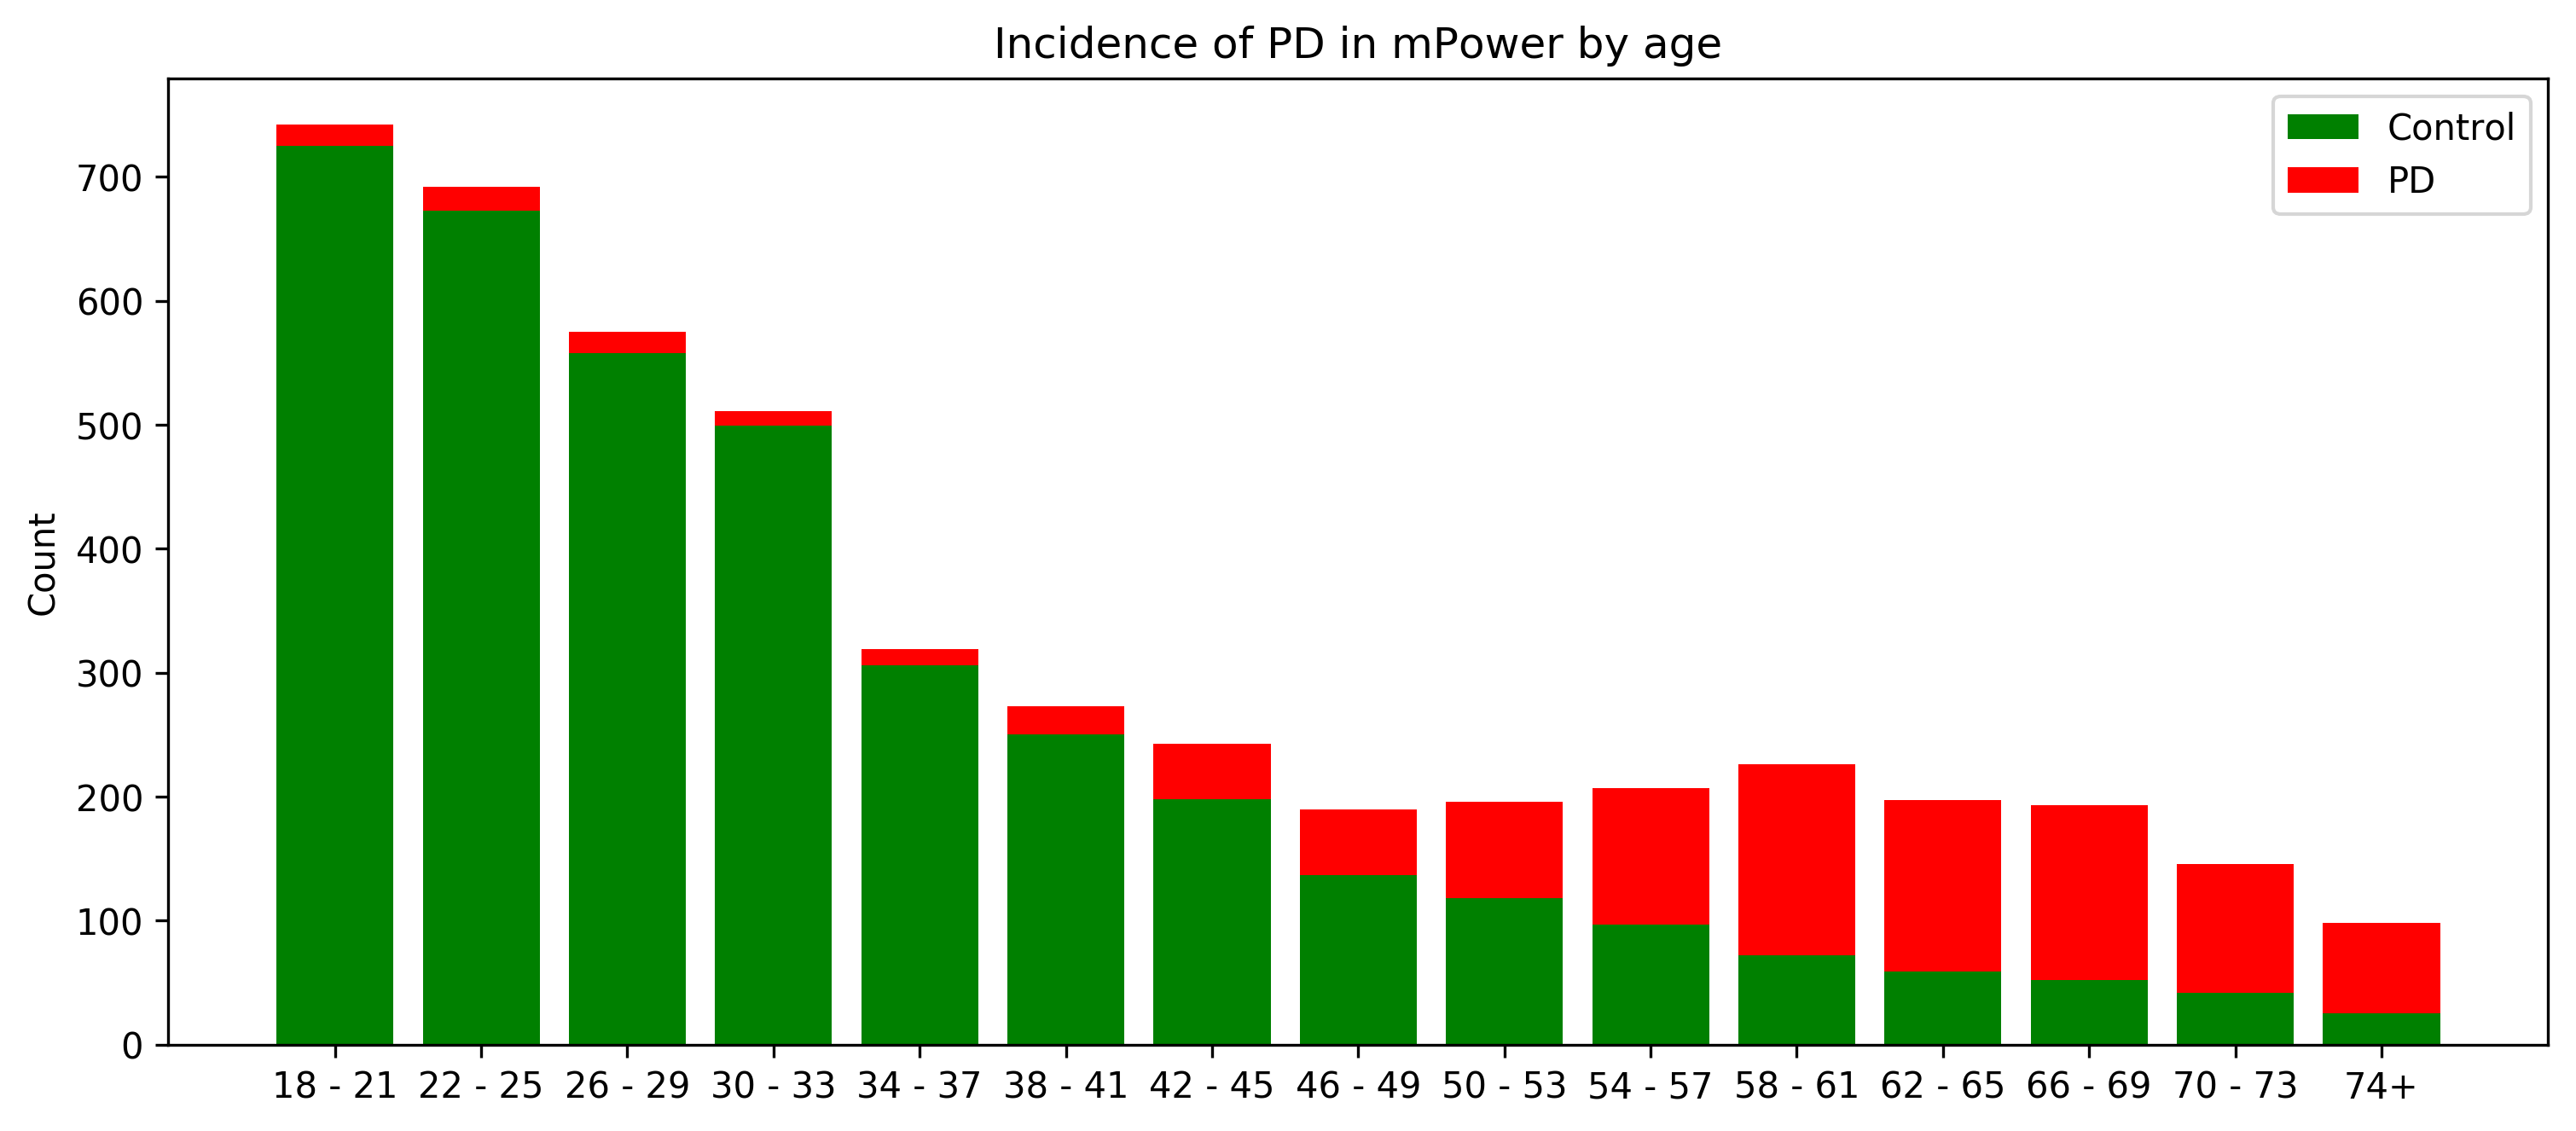
\includegraphics[width=1\linewidth]{mpowerage.png}
\caption{Age is a bias in the mPower dataset as most non-PD participants are young. There are also some cases of rare young-onset PD\protect\footnotemark.}
\end{figure}

%The mPower data study was an experiment in data-collection and was not created with machine learning as a focus. 
Despite the dataset being released to the public in early 2016 and having multiple citations from machine learning and clinical papers, there has been no machine learning study published using the mPower data. The primary issue with the data is that it is quite `noisy' --- a major issue with any crowdsourcing project without significant precautions~\cite{crowdsourcing}. 

\subsection{Preprocessing and Feature Selection.}
\label{mpowerprocess}
\emph{Vowel phonation} was captured with the single channel iPhone/iPod microphone at 44,100 Hz. Initial investigation showed that a substantial number of participants did not complete the task to an acceptable standard. Although the mPower application prevented access to the voice task when background noise exceeded a certain threshold, this threshold was too lenient. A large number of participants also failed to complete the recording task properly --- hesitation, interruptions and pronouncing vowels other than `aaaaah...' were common. There was also a large variation in the distance to the phone during recording with some participants speaking directly into the microphone creating a large amount of `wind noise'~\cite{windnoise}. 

At the time of writing, there were 65,000 speech samples from 6,000 subjects in the mPower dataset (a majority of these from a small number of users). We evaluated approximately 2,000 randomly selected samples for performing the task correctly and having acceptable levels of background noise, rejecting around 25\%. Simple metrics such as variance in short time energy and noise prior to recording were used in hand-crafted rules to rank and filter the speech samples. After filtering, 4,100 users remained, 900 with PD. The highest ranked speech sample was selected for each of the users\footnote{Optimally, all samples should be used to improve robustness, however available processing power was limited.}. Machine learning could optimize this process, however it was avoided due to the possibility of introducing bias to the data. 

The \emph{walking} task involves the participant putting their phone in the pocket or bag, walking 20 steps then standing still for 30 seconds. During this task, accelerometer and gyroscope data is continually collected at 95$\pm$7 Hz. Although in-pocket IMU gait estimation exists~\cite{diaz2014step}, mPower does not record the parameters necessary (such as leg length) to estimate parameters other than cadence. The results of Esser~et~al.~(2011)~\cite{esser2011assessment} suggests that although PD patients on average have a longer cadence, the separation is not clean.

The standing task is therefore more interesting in the context of machine learning. As the device is in the user's pocket or bag, data from the gyroscope would be minimally informative. Using gyroscope data, a rotation matrix was calculated to align the accelerometer's $z$ axis to the direction of gravity. 

\begin{figure}[h]
\label{mpowerwalking}
\centering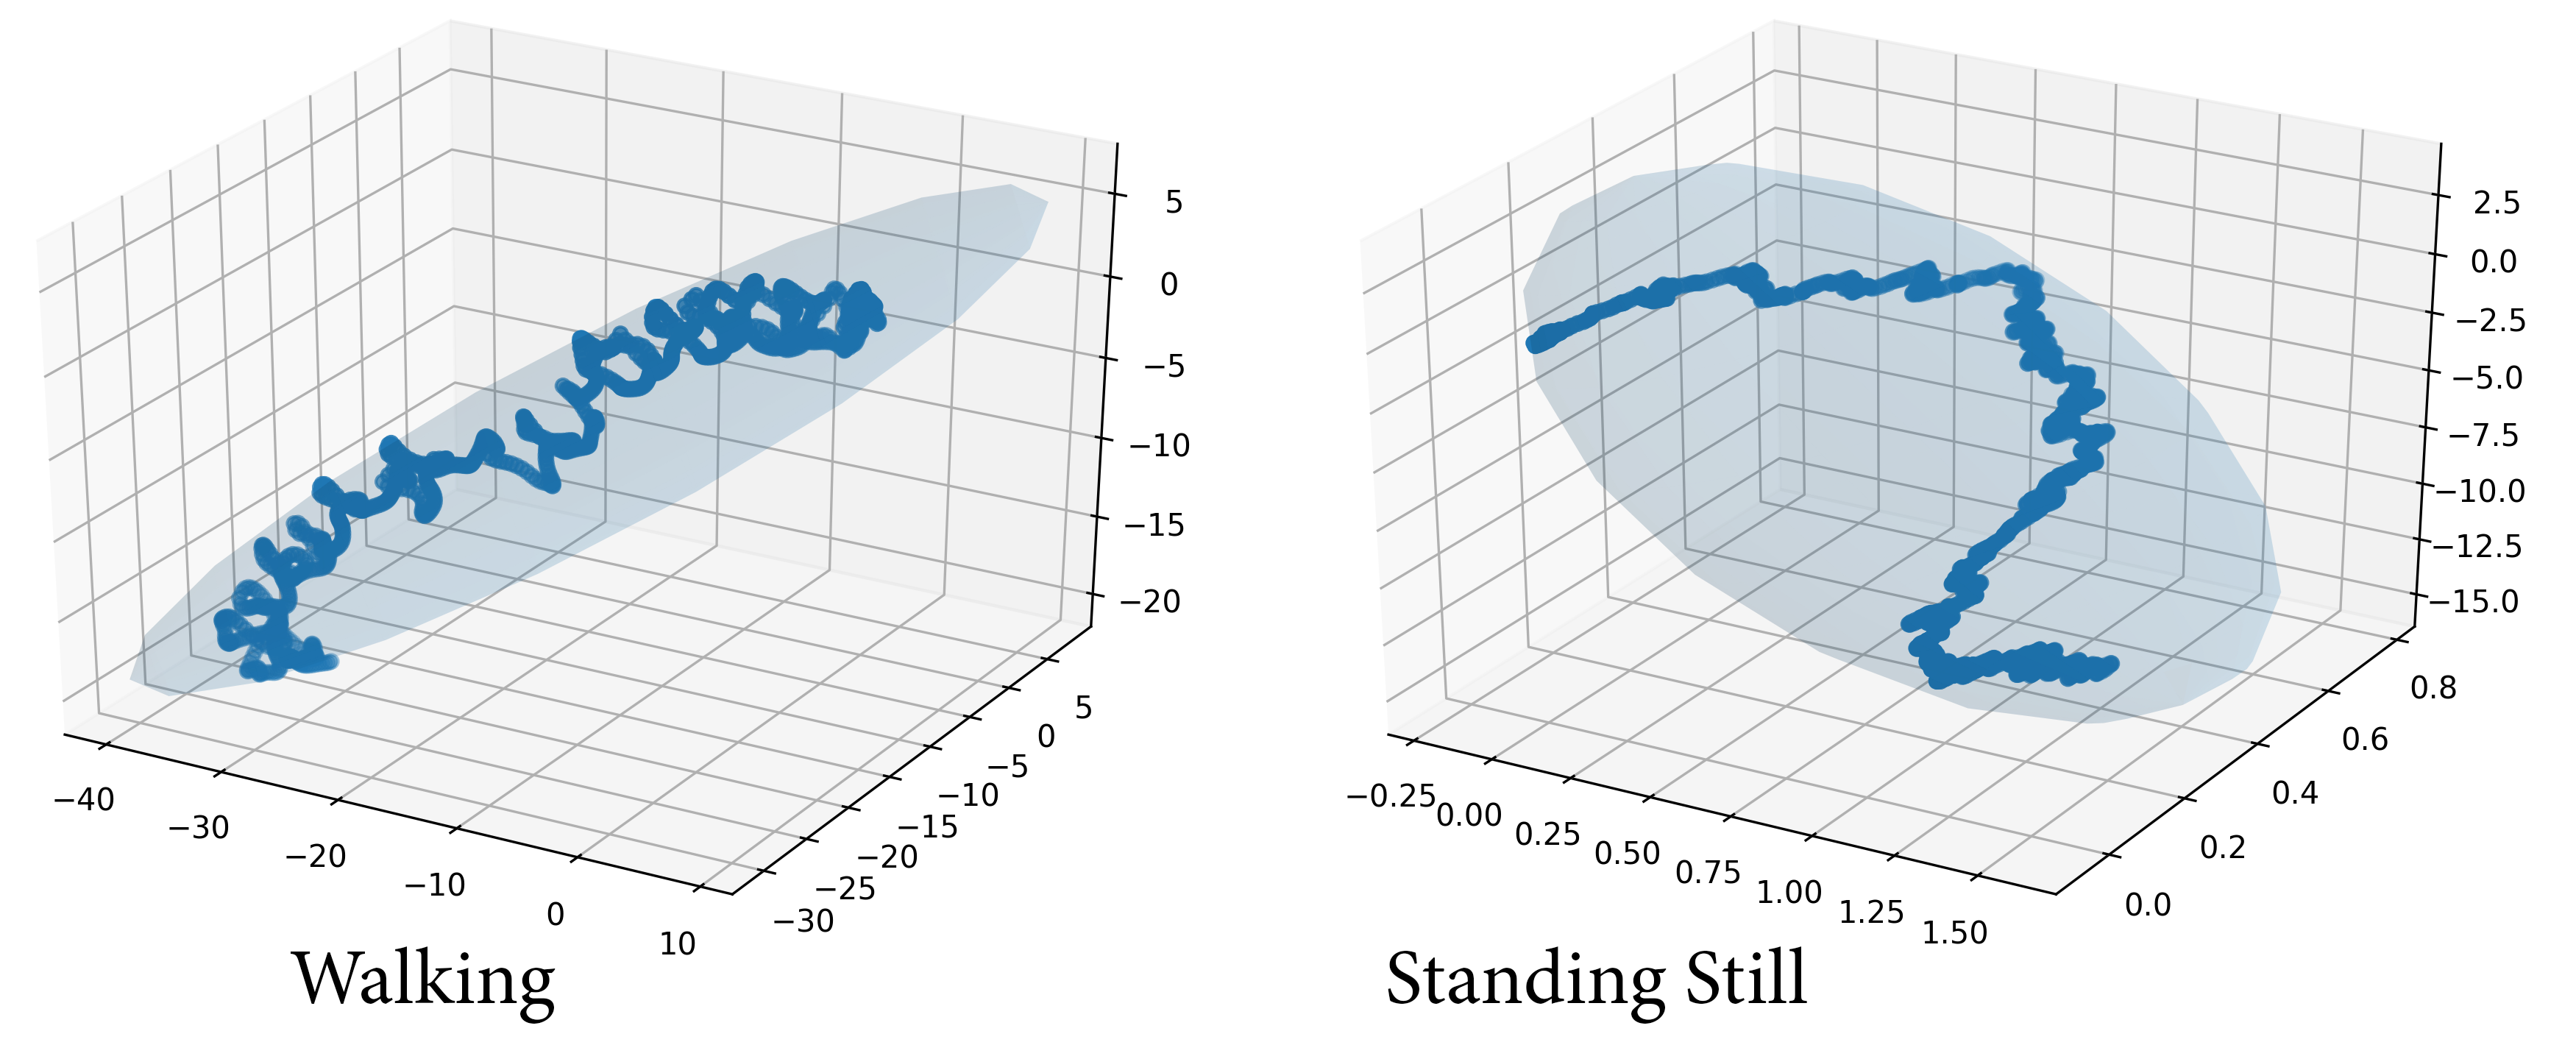
\includegraphics[width=0.8\linewidth]{pathvis3d.png}
\caption{A visualisation of device position after correcting for rotation with a bounding ellipsoid at 95\% CI. Gravity ($z$) is not subtracted.}
\end{figure}

Unlike similar experiments carried out in force plates, the subject was not instructed to stand as still as possible. A majority of subjects show a significant amount of sway which could be consciously preventable. To map the accelerometer data more closely to force plate data, a 10\textsuperscript{th} order zero-phase 1hz Butterworth highpass filter was applied. The highpass filter removes preventable sway at the cost of removing valuable sway information below 1hz~\cite{swayspectral}. 

A 16 second extract of rest data between 4s and 20s and the first 10 seconds of the walking task were used for each subject for feature extraction. The choice of these values were solely informed by the nature of the dataset, with the first four seconds of rest data containing significant movement and most recordings of variable length. Features specified in section~\ref{featuresummary} were extracted using the tools and techniques specified in section~\ref{implementationfeature}.  Feature Extraction was done on both the original and filtered data for the resting task and only unfiltered for the walking task. The motion data was then filtered and ranked based on simple criterion such as average acceleration and the best selected for each subject.

\begin{figure}[h]
\label{butterworth}
\centering\centerline{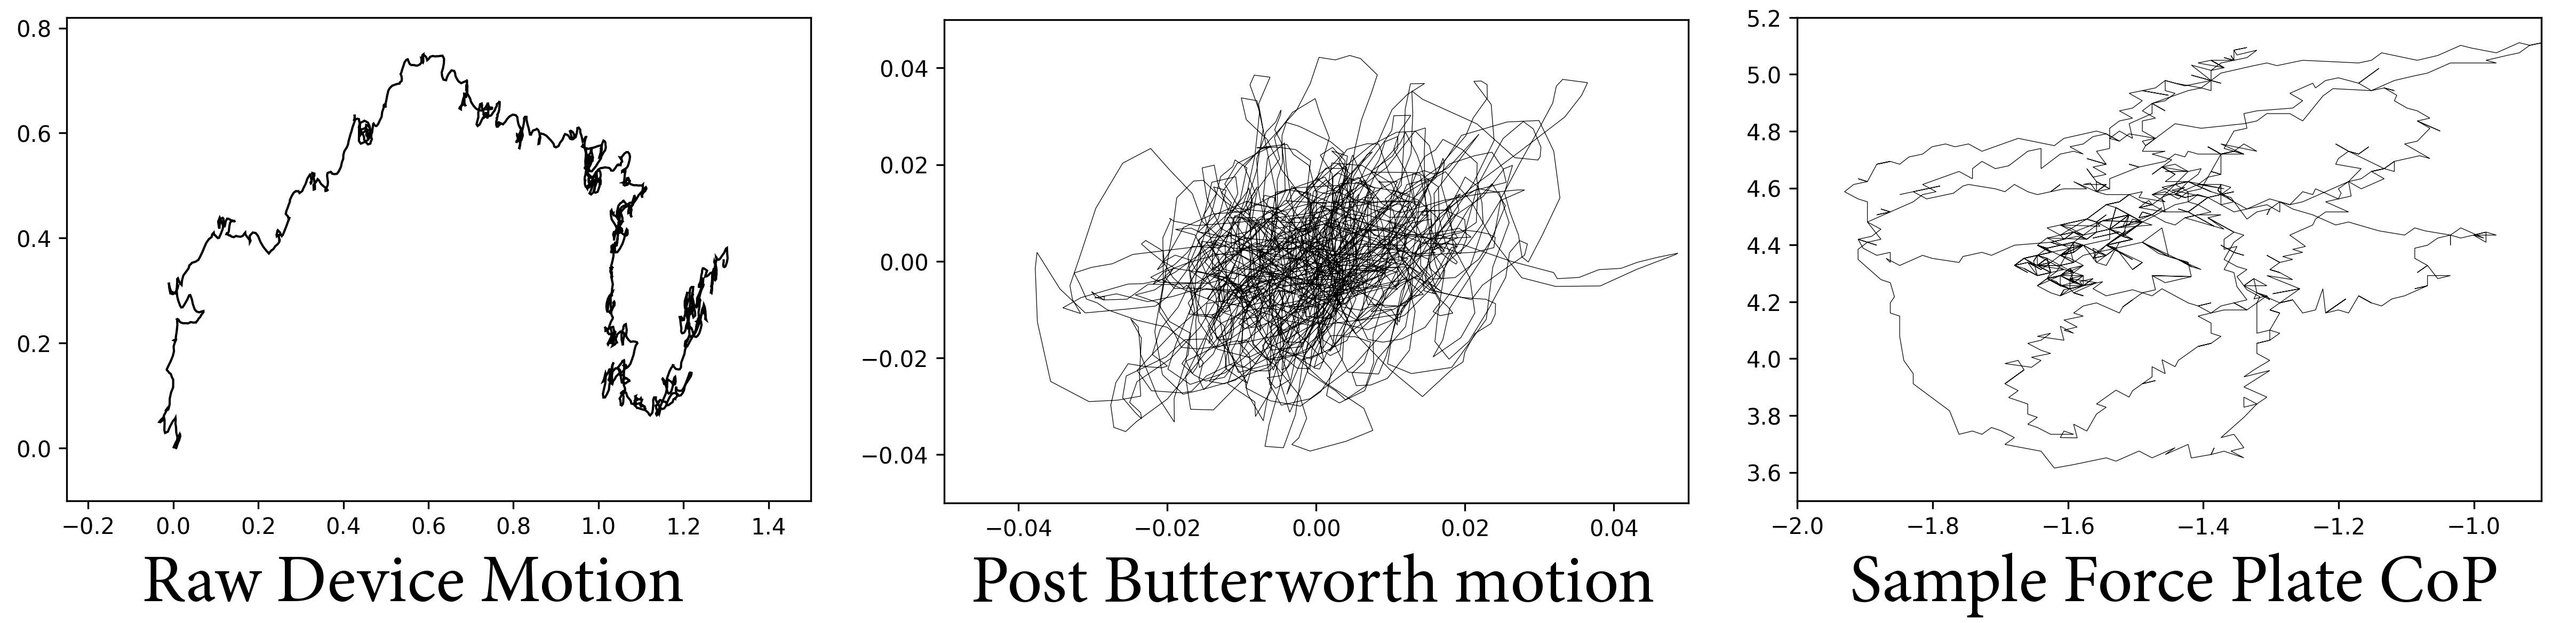
\includegraphics[width=1.1\linewidth]{butterworth.png}}
\caption{The Butterworth filter results in a device path more similar to the centre of pressure, however low frequency sway information is lost. Note that the device motion recording is 30 seconds long while the force plate is 10 seconds.}
\end{figure}


\section{Replicating Past Work}
The two key results we will be replicating on the mPower dataset are the 98.6\% accuracy from vowel phonation reported in Tsanas et~al.~(2011)~\cite{tsanas2012novel} and the 98.0\% accuracy with smartphone accelerometer data reported by Arora et~al.~(2014)~\cite{arora2014high}. 

\subsection{Vowel Phonation}
Tsanas et~al.~(2012)~\cite{tsanas2011nonlinear} uses the National Center for Voice and Speech (NCVS) dataset which consists of 33 people with PD and 10 healthy controls. 263 phonations in total were recorded in controlled circumstances using a professional grade microphone. HNR, GQ, RPDE, DFA, PPE, GNE, VFER, EMD-ER, MFCC and variants of shimmer and jitter were extracted, resulting in a set of 132 features (See \ref{featuresummary}).

Features were calculated on the 263 phonations and 10 fold, 100 repetition cross validation used for evaluation of models. It is unclear whether Tsanas~et~al. has split the phonations on a per-subject scale. Failure to do so presents a high risk of overfitting as two phonations from the same subject may appear in both the training and validation set. Random Forests and SVMs were evaluated with hyperparameters selected by gridsearch~\cite{gridsearch}. As data is limited, feature selection with four common algorithms was performed to improve results. This results in the 10 feature subsets depicted in figure \ref{tsanasresults}.

\begin{highlight}
It is unclear whether Tsanas~et~al. has split the phonations on a per-subject scale and failure to do so presents high risk of overfitting.
\end{highlight}

\begin{figure}[h]
\caption{Cross-validation accuracy of Tsanas et~al. with a SVM classifier after feature selection. Results reported as mean accuracy $\pm$ std accuracy.}
\label{tsanasresults}
\centering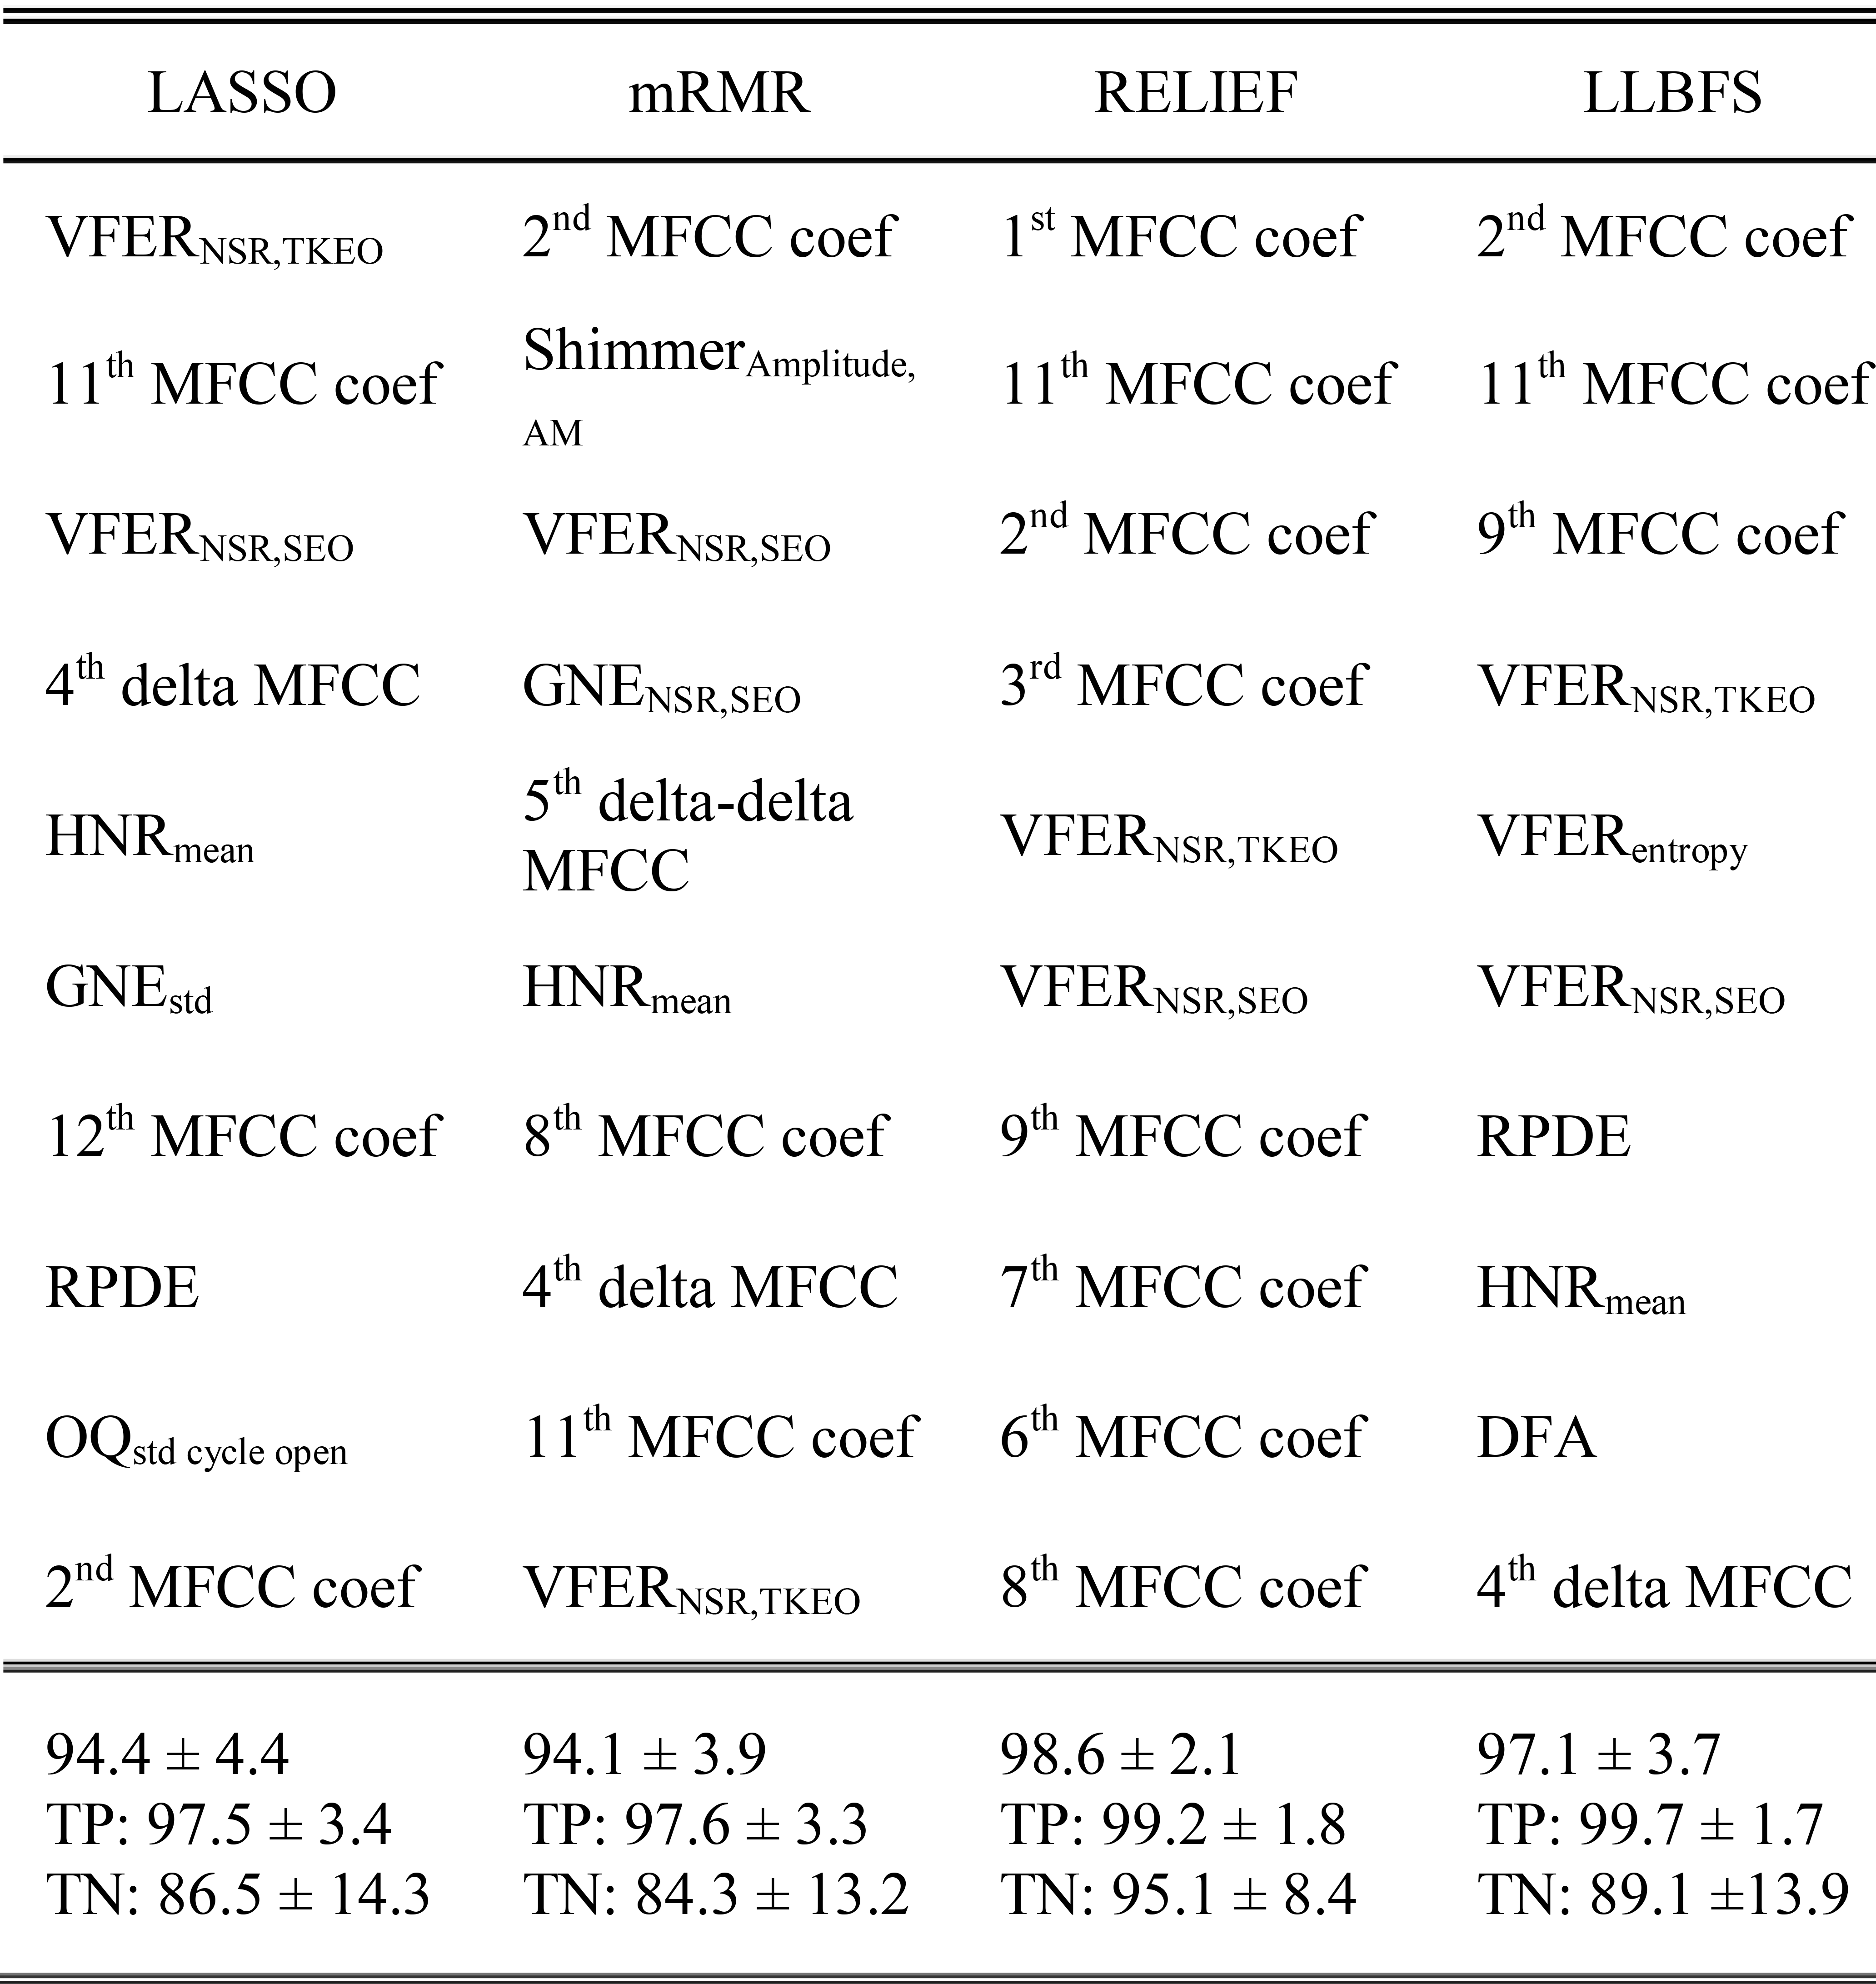
\includegraphics[width=0.75\linewidth]{tsanas.png}
\end{figure}
 
We replicated Tsanas et~al. on the 4,100 phonation samples selected after preprocessing mPower (see \ref{mpowerprocess}). Features were extracted from a 2 second window was of each audio sample which mirrors the phonation length used in fundamental frequency estimation datasets~\cite{tsanas2014robust}. Gridsearch was performed to find (near) optimal SVM hyperparameters. The best performing feature subset of Tsanas et~al., extracted with the ReliefF algorithm is initially evaluated.

Note that the NCVS data used in Tsanas et~al. is at a ratio of 33PD:10C whereas the mPower data is at a ratio of approximately 9PD:32C. We stratify the data by random sampling to simulate NCVS split. On both the NCVS and mPower ratio, the SVM classifier exhibits the false positive paradox, where the most common class is predicted for all inputs. The results are summarised in table \ref{tsanasfsresults}.

\begin{table}[h]
\caption{Cross validation results of optimal SVM from random search using Tsanas' 10 feature ReliefF subset. Presented as mean $\pm$ stdev.}
\label{tsanasfsresultsrelieff}
\centering
\begin{tabular}[t]{c c c}
{\specialcellbold{Equal Split (50P:50C)}} &&
{\specialcellbold{NCVS Split (33P:10C) }} \\[10pt]
\begin{tabular}{lcl}\hhline{~|*{2}{-}}
	\multicolumn{1}{l|}{}                                 & \multicolumn{1}{l|}{\cellcolor[HTML]{EFEFEF}Pred PD} & \multicolumn{1}{l|}{\cellcolor[HTML]{EFEFEF}Pred C} \\ \hline
	\multicolumn{1}{|l|}{\cellcolor[HTML]{EFEFEF}True PD} & \multicolumn{1}{c|}{$30.1\pm2.5$\%}                          & \multicolumn{1}{c|}{$20.0\pm2.5$\%}                         \\ \hline
	\multicolumn{1}{|l|}{\cellcolor[HTML]{EFEFEF}True C}  & \multicolumn{1}{c|}{$15.1\pm2.5$\%}                          & \multicolumn{1}{c|}{$34.9\pm2.5$\%}                         \\ \hline
	\multicolumn{2}{l}{Accuracy}                                                                                 & $65.0\pm3.3$\%                                              \\
	\multicolumn{2}{l}{Sensitivity (TP)}                                                                         & $60.1\pm5.0$\%                                              \\
	\multicolumn{2}{l}{Specificity (TN)}                                                                         & $69.8\pm5.0$\%                                             
\end{tabular}
& &
\begin{tabular}{lcl}\hhline{~|*{2}{-}}
\multicolumn{1}{l|}{}                                 & \multicolumn{1}{l|}{\cellcolor[HTML]{EFEFEF}Pred PD} & \multicolumn{1}{l|}{\cellcolor[HTML]{EFEFEF}Pred C} \\ \hline
\multicolumn{1}{|l|}{\cellcolor[HTML]{EFEFEF}True PD} & \multicolumn{1}{c|}{$76.7\pm0$\%}                          & \multicolumn{1}{c|}{$0\pm0$\%}                         \\ \hline
\multicolumn{1}{|l|}{\cellcolor[HTML]{EFEFEF}True C}  & \multicolumn{1}{c|}{$23.3\pm0$\%}                          & \multicolumn{1}{c|}{$0\pm0$\%}                         \\ \hline
\multicolumn{2}{l}{Accuracy}                                                                                 & $76.7\pm0$\%                                              \\
\multicolumn{2}{l}{Sensitivity (TP)}                                                                         & $100\pm0$\%                                              \\
\multicolumn{2}{l}{Specificity (TN)}                                                                         & $0\pm0$\%                                             
\end{tabular}
\end{tabular}
\end{table}
The results using the mPower dataset are evidently poorer than the reported 98.6\% accuracy. The ReliefF~\cite{relieff} feature subset consists primarily of MFCC coefficients. MFCC is a very powerful feature and is often the primary feature in speech recognition systems. The high and low MFCC coefficients are known to be rarely informative in speech recognition~\cite{mfcchistory} and the ReliefF feature set contains both the 1\textsuperscript{st} and 11\textsuperscript{th} coefficients. The result suggest that these coefficients may be informative when used to detect abnormal speech and more MFCC coefficients should be extracted~\cite{mfcc}. MFCC are known for being very sensitive to noise and frequency~\cite{mfccrobust,mfccrobust2}. Tsanas~et~al. used professional grade microphones whereas mPower audio data is recorded with a smartphone microphone; 

Another possibility is overfitting. It is ambiguous if Tsanas~et~al. divided phonations of a per-subject level in cross validation. Naive CV may result in  phonations from same individuals appearing in both the training and validation sets. As MFCCs are sensitive to minor changes in frequency~\cite{mfccrobust2}, phonations from different individuals are likely easily separable in the MFCC space. This is also supported by the disparity of results between the Random Forest and SVM classifiers on all features (90.2\% vs 97.7\%) as the hyperparameters of the RF classifier were not tuned by cross validation and RF is generally more robust against overfitting. 

In our testing, using all measures presented in Tsanas~et~al. results in improvements over any of the 10 feature subsets presented in figure \ref{tsanasresults}.

\begin{table}[h]
	\caption{Mean Cross validation results of optimal SVM from random search using all features presented in Tsanas~et~al. (2012)~\cite{tsanas2012novel}. Outperforms \ref{tsanasfsresultsrelieff} with a Bayes factor of $10^{17}$.}
	\label{tsanasfsresults}
	\centering
	\begin{tabular}[t]{c c c}
		{\specialcellbold{Equal Split (50P:50C)}} & &
		{\specialcellbold{mPower Split (9P:32C) }} \\[10pt]
		\begin{tabular}{lcl}\hhline{~|*{2}{-}}
			\multicolumn{1}{l|}{}                                 & \multicolumn{1}{l|}{\cellcolor[HTML]{EFEFEF}Pred PD} & \multicolumn{1}{l|}{\cellcolor[HTML]{EFEFEF}Pred C} \\ \hline
			\multicolumn{1}{|l|}{\cellcolor[HTML]{EFEFEF}True PD} & \multicolumn{1}{c|}{$32.4\pm2.8$\%}                          & \multicolumn{1}{c|}{$17.6\pm2.8$\%}                         \\ \hline
			\multicolumn{1}{|l|}{\cellcolor[HTML]{EFEFEF}True C}  & \multicolumn{1}{c|}{$13.9\pm2.4$\%}                          & \multicolumn{1}{c|}{$36.1\pm2.4$\%}                         \\ \hline
			\multicolumn{2}{l}{Accuracy}                                                                                 & 68.4$\pm$3.9\%                                              \\
			\multicolumn{2}{l}{Sensitivity (TP)}                                                                         & 64.7$\pm$5.6\%                                              \\
			\multicolumn{2}{l}{Specificity (TN)}                                                                         & 72.1$\pm$4.8\%                                             
		\end{tabular}
		& &
		\begin{tabular}{lcl}\hhline{~|*{2}{-}}
			\multicolumn{1}{l|}{}                                 & \multicolumn{1}{l|}{\cellcolor[HTML]{EFEFEF}Pred PD} & \multicolumn{1}{l|}{\cellcolor[HTML]{EFEFEF}Pred C} \\ \hline
			\multicolumn{1}{|l|}{\cellcolor[HTML]{EFEFEF}True PD} & \multicolumn{1}{c|}{$3.4\pm0.8$\%}                          & \multicolumn{1}{c|}{$17.6\pm0.8$\%}                         \\ \hline
			\multicolumn{1}{|l|}{\cellcolor[HTML]{EFEFEF}True C}  & \multicolumn{1}{c|}{$1.7\pm0.7$\%}                          & \multicolumn{1}{c|}{$77.3\pm0.7$\%}                         \\ \hline
			\multicolumn{2}{l}{Accuracy}                                                                                 & $80.7\pm1.0$\%                                              \\
			\multicolumn{2}{l}{Sensitivity (TP)}                                                                         & $16.1\pm3.7$\%                                              \\
			\multicolumn{2}{l}{Specificity (TN)}                                                                         & $97.8\pm0.9$\%                                             
		\end{tabular}
	\end{tabular}
\end{table}


\subsection{Movement}
Arora et al.~\cite{arora2014high} conducted a study with 10 control and 10 PD participants, obtaining 98.0\% accuracy on 10 fold cross validation with 100 repeats on accelerometer data alone. Participants were provided with a LG Optimus S smartphone and instructed to walk 20 steps, turn around, walk 20 steps then 
stand upright for 30 seconds. The position of the device was not specified however it can be assumed to be in the participant's pocket. No preprocessing was done to the data, and features extracted included simple statistical and entropy measures, DFA, mean TKEO and the dominant frequency. It should be noted that Zhan et al~\cite{zhan2016high} extended the dataset and performed a similar experiment on 121 PD and 105 control using additional voice and tapping features, however only achieved 71.0\% accuracy.

This thesis coincides with the Parkinson's Disease Digital Biomarker DREAM Challenge which involves using accelerometer data to classify PD or predict the UPDRS motor score~\cite{dreamchallengeinfo}. Sage Bionetworks, sponsor of the mPower dataset and a organiser for the challenge released a baseline feature set~\cite{mpowertools} which included all features in Arora et al~\cite{arora2014high} and additional jerk based measures and the peak of the Lomb-Scargle periodogram~\cite{lombscargle}. The work completed as part of this thesis was submitted to the challenge, earning Xth place. The challenge evaluated the trained models on an unreleased portion of the mPower data, validating that our models have not overfit.

After filtering out samples which are too short (<10 seconds), have too much variability in recording rate or are missing measurements, XXXX people remain with a valid walk recording. The most recent valid walk was selected for each patient and all relevant features specified in section~\ref{featuresummary} extracted. 

Before 


\section{Dynamical Systems Features and Data Boosting}
\label{databoosting}
We decided to investigate the potential of traditional 	


\section{Visualising The Features}
The models replicated in the previous sections clearly perform below the reported level in prior works. This disparity is possibly caused by differences in dataset quality, particularly in ensuring that the task is performed correctly or consistently. It is also likely that introducing a greater diversity of subjects increases the problem difficulty as there are natural variances in speech and gait. No individual feature was able to achieve greater than 60\% classification accuracy on an equal split of the data. 

\subsection{Speech}
A large number of dysphonia related measures rely on precise measurements of the length of each glottal cycle. The SWIPE~\cite{camacho2007swipe} fundamental frequency estimation algorithm was primarily used to obtain these measurements. Most $f_0$ algorithms are sensitive to changes and noise in the signal and are not yet suitable to handle the noisy mPower data gathered in real-world conditions. Issues with $f_0$ extraction would invalidate the measurements from $f_0$ based signal processing. A simple investigation shows that the standard deviation of $f_0$ exceeds 10Hz for 347 subjects, a value that is almost certainly indicates a failure of the algorithm or a poorly executed recording.

\begin{figure}[h]
	\caption{Standard Deviation of the fundamental frequency during vowel phonation. Females and older individuals exhibit notably higher variations in $f_0$. People with PD seem to exhibit an increased variation in $f_0$ compared to age matched control subjects, however the distinction is less clear.}
	\centering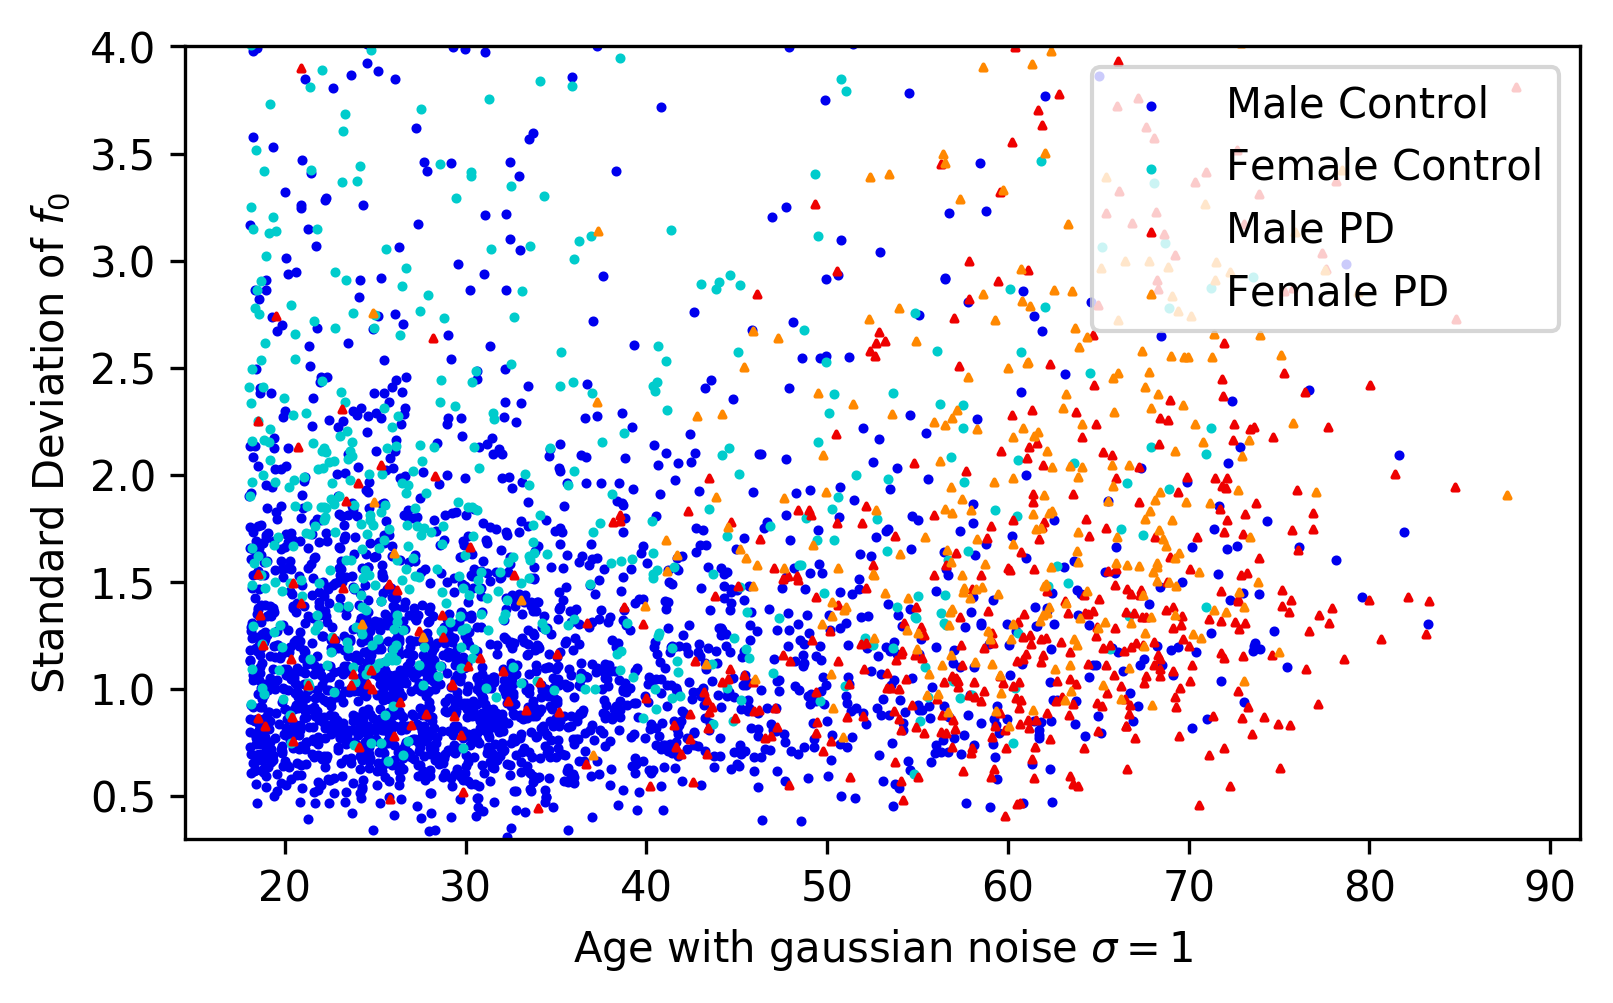
\includegraphics[width=0.75\linewidth]{f0stdev.png}
\end{figure}

Little~et~al.~\cite{splittlenonlinear2007,splittledysphonia2009} introduces three measures to distinguish dysphonia --- DFA, RPDE and PPE. DFA and RPDE are measured of the autocorrelation of a signal. As evident in figure \ref{dfapperpde}, people with PD exhibit a lower autocorrelation than age matched control subjects, indicative of a more chaotic and variable speech signal. People with PD also show an increase in PPE to age matched control, which is evidence of fluctuations in pitch above healthy speech production. However, the natural variance in speech production makes distinguishing dysphonic speech difficult.


\begin{figure}[h]
	\caption{PD subjects exhibit a lower DFA and RPDE, and a higher PPE. However these features are hardly separable.}
	\label{dfapperpde}
	\centering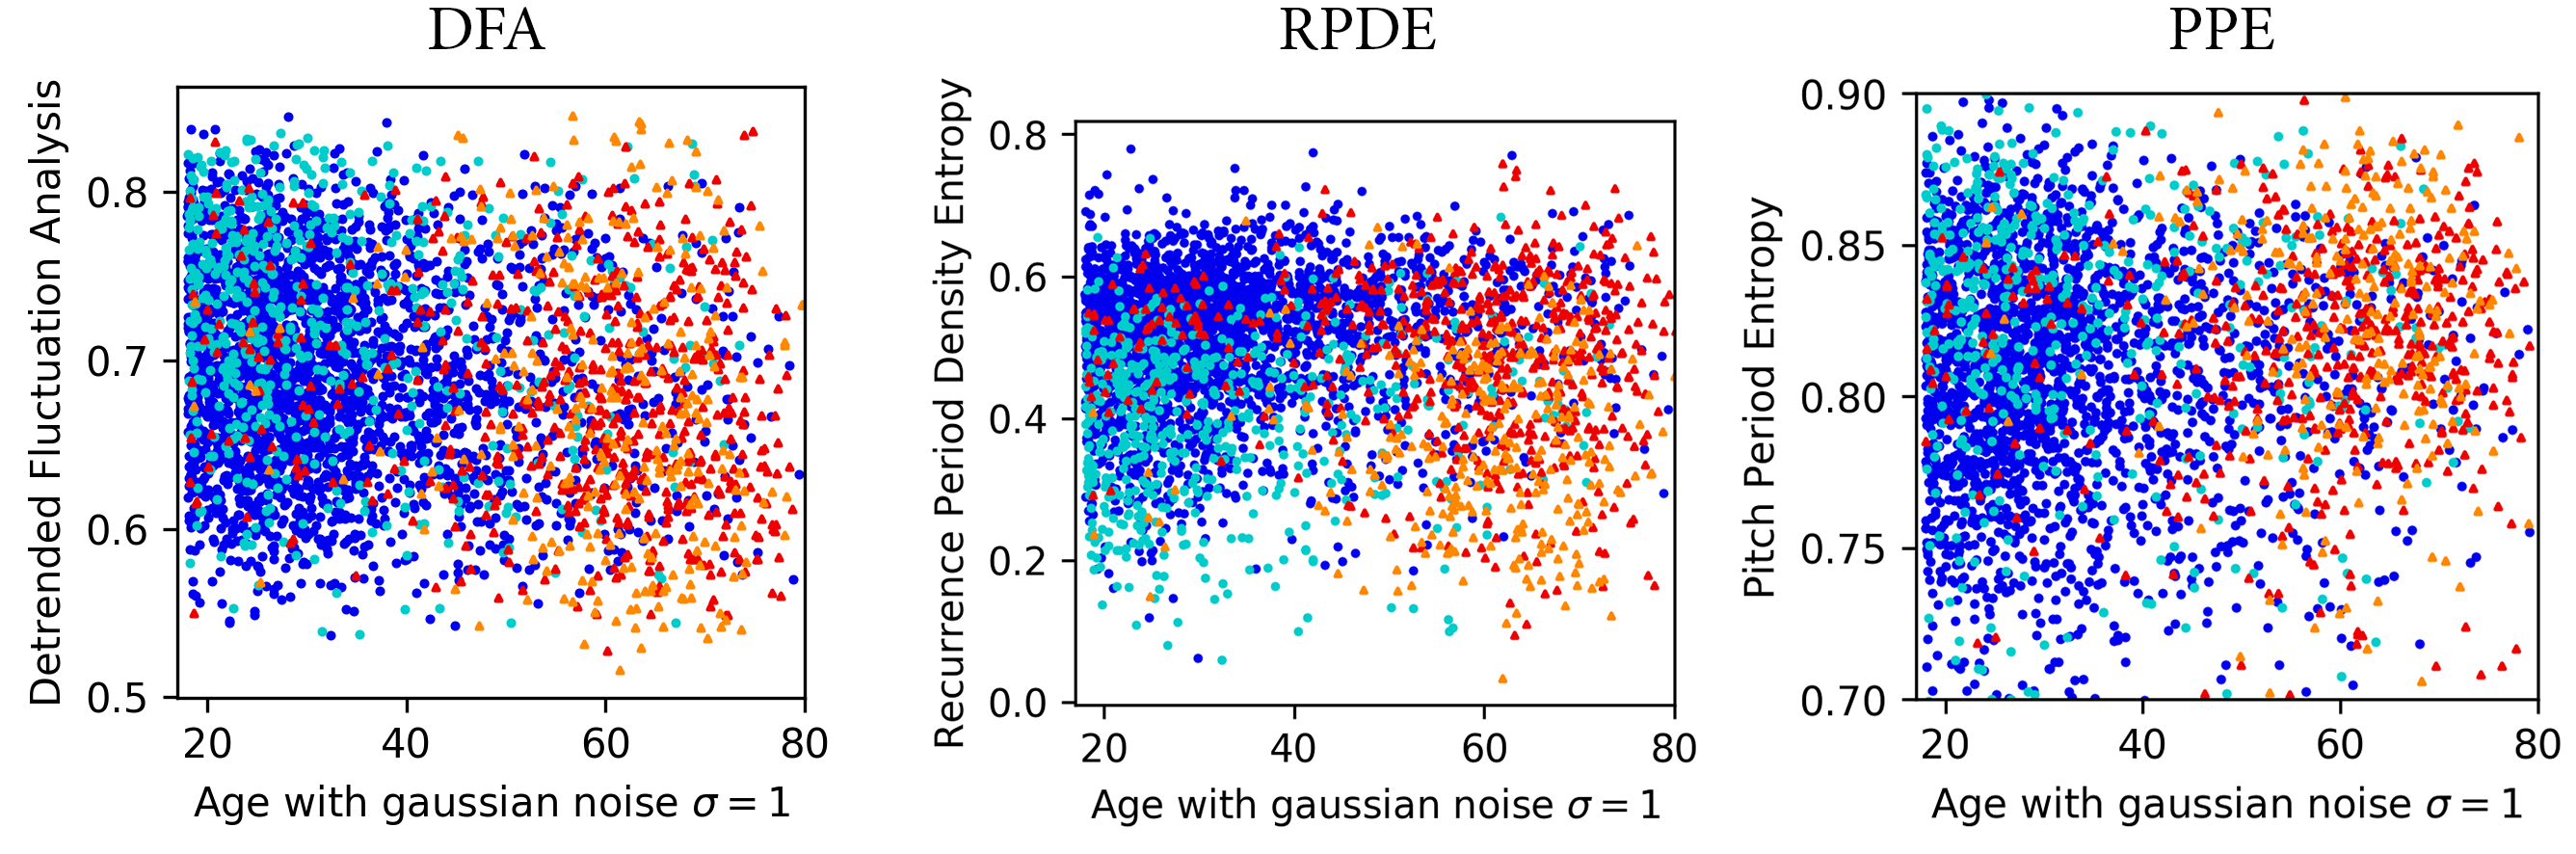
\includegraphics[width=1\linewidth]{dfapperpde.png}
\end{figure}


Benba et~al.~\cite{benba2014mfcc} distinguishes PD with a 82\% success rate primarily with MFCC. The MFCC are also present in most of the feature subsets derived by Tsanas et~al.~\cite{tsanas2012novel}. MFCC are the primary feature in most speech recognition systems so it is not surprising they are strong features in detecting dysphonia. However, figure \ref{mfcc_feat} suggests that there is a very minimal correlation between mean and standard deviation measures of the MFCC and the occurrence of PD. The MFCC are very sensitive to changes in the signal, and more advanced measures than the mean and standard deviation may be required to fully utilise them. This will be explored in section \ref{automaticfeatureextraction}.


\begin{figure}[h]
	\caption{The 8\textsuperscript{th} MFCC coefficient is not a particularly notable feature for distinguishing dysphonia. The visualisation of other coefficients appear roughly the same. }
	\label{mfcc_feat}
	\centering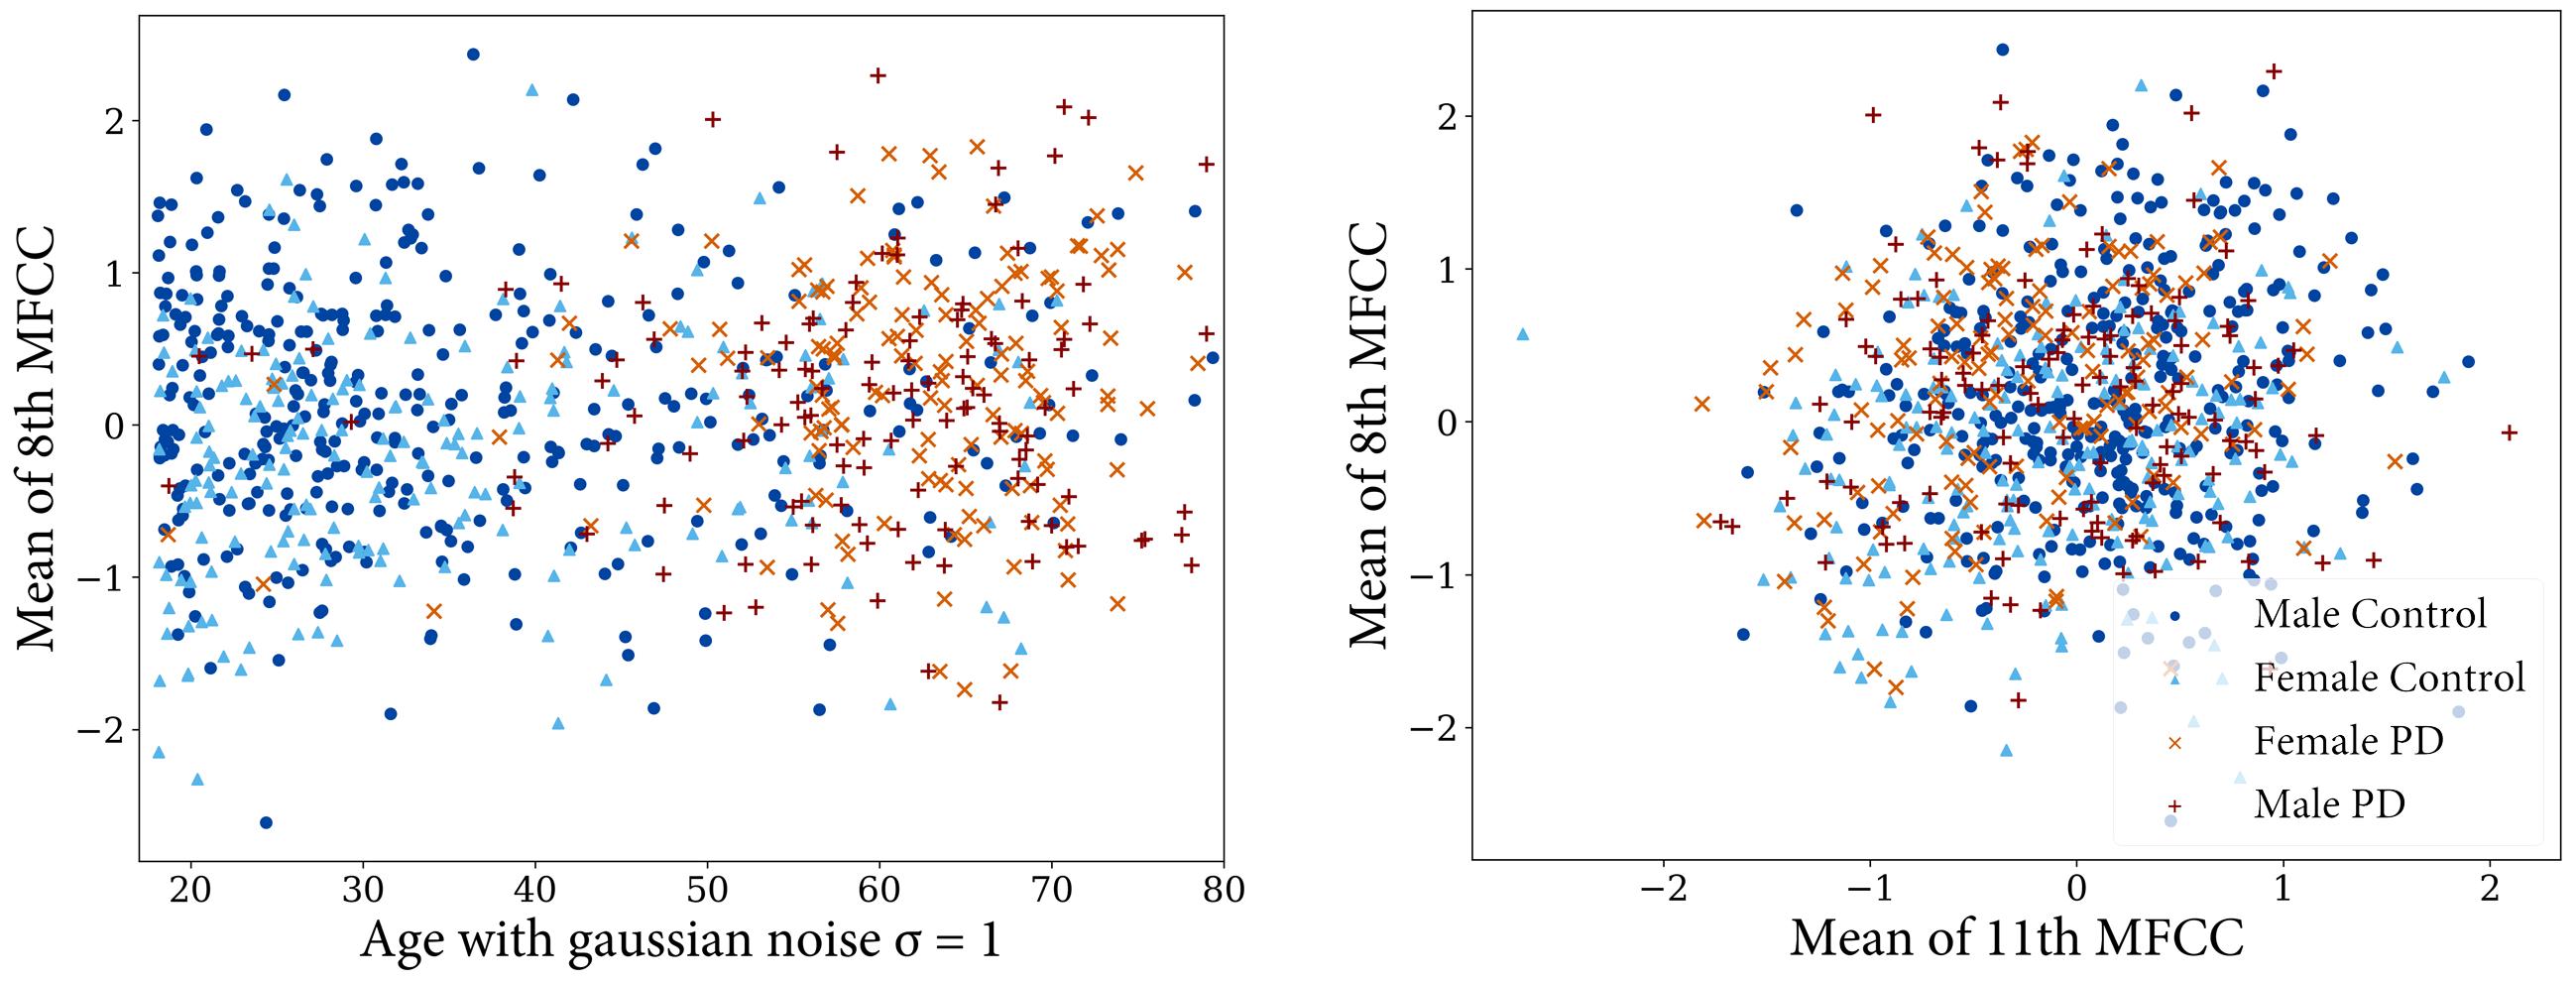
\includegraphics[width=1\linewidth]{mfcc_feat.png}
\end{figure}

YYYY was one of the stronger features in distinguishing



\subsection{Movement}



\subsection{Conclusions and Recommendations}
\label{visfeatrecommendations}
The wide variation in natural speech production makes it difficult to clearly distinguish dysphonic speech. Many features are not invariant to the fundamental frequency of the speaker as evident in the clear differences between the male and female groups. Investigating and normalising these features with respect to $f_0$ would likely improve the applicability of these features.

Many features are very sensitive to minor fluctuations in the signal and their value can change dramatically depending on the segment used, as shown in section~\ref{databoosting}. The large fluctuations in value reduces their effectiveness in simple predictors, however these may be valuable when the feature is extracted over short-time intervals. Models such as CNNs or LSTMs (ref \ref{neuralnetworkintro}) can utilise the additional temporal information and make more robust predictions. This would also solve the issue of some features being dependent on data length. Unfortunately this will not be explored due to computational limitations.

As no individual feature can achieve good classification accuracy, the machine learning model must combine multiple features to reach a reasonable level of performance. Traditional machine learning models are best suited to modelling features which are independent and often perform worse when two features are correlated despite there being additional information. Feature selection~\cite{skfeature} can be used in traditional machine learning models to reduce the impact of this however information is definitely lost. It is possible that non-linear models such as neural network may be able to utilise more of this information, however a lot of training data will be required.



\section{Automatic Feature Extraction: Neural Networks}
\label{automaticfeatureextraction}
A notable weakness of traditional machine learning to feature extraction is that information is often lost in the process as it is difficult for features to perfectly describe a signal. As evident in computer vision and EEG signal processing~\cite{bashivan2015learning}, CNN and LSTM based neural network architectures present a viable solution, automatically `learning' the best features from a more raw representation of the data. 

The biggest tradeoff in using automatic feature engineering is that understanding the features extracted is a bigger investment than developing the model. A great deal of trust must be placed on the model and that it has not conveniently overfit on the dataset. However, diagnosing PD is a difficult enough task such that many features are already difficult to understand. As explored in section \ref{visfeatrecommendations}, no individual feature is a good quantifier of PD and an similarly difficult to interpret model must be used to fit these uncertain features.

The architectures we developed 

WALK:: USE SUPPL trained model
TALK:: USE CROSS VAL.

features unclear.

add noise and understand what happens -- what do the numbers represent, if anything?



Computational power may have been too limited
Due to the sensitivity of some features, it would be very interesting to extract all features on a short time scale and use a LSTM to observe
however computational resources were too limited. 

\section{The Power of Machine Learning}

There are a non-linearities


medication on off --- difference diagnosis. Would be useful in real world diagnosis.

Most sensors can only measure a small 

to the quality of the machine learning model. 


In this thesis we setup experiments to provide evidence of machine learning's ability to classify PD and control patients. Experiments involve:

\section{Implementation}
\label{implementation}
We would like to extend our thanks to all open-source libraries and academics making their code publicly available. Without these, development would have been a significantly slower process. 

The project was primarily implemented in Python, acting as an interface between a number of libraries written in C, R (rpy2) and Matlab (Matlab Engine). The code for this project is made available .... under the CRAPL license???

Wherever possible, reliable standard libraries or implementations used in previous research were preferred to maximise reproducibility and reliability. Standard speech features used in Interspeech were extracted using the official openSMILE~\cite{opensmile} program, which uses the sub-harmonic summation method of $f_0$ estimation~\cite{shs}. Most dysphonia-specific features were extracted using Tsanas' toolbox~\cite{spoverview} with the SWIPE~\cite{camacho2007swipe,f0estimation} $f_0$ estimation algorithm. Following Tsanas~(2012)~\cite{spoverview}, 120hz and 190hz were used as the mean healthy $f_0$ for males and females respectively. The Toolbox features code for DFA and RPDE which were proposed and implemented by Little~(2007)~\cite{splittlenonlinear2007} which were also used in processing the walking code.

EEG and non-linear signal analysis was performed using the PyREM library~\cite{pyrem}, which builds upon PyEEG~\cite{pyeeg}, correcting some implementation flaws. The false nearest neighbour implementation in the pypsr~\cite{pypsr} library was used to calculate the embedding dimension for the relevant non-linear signal processing algorithms. The embedding dimension chosen for accelerometer data was 6, and speech 4.
 
Features were 
Jerk was considered~\cite{jerkfeature}


Most traditional machine learning algorithms were based on the standard scikit-learn~\cite{scikitlearn} implementation and Gaussian processes implemented with GPy~\cite{gpy2014}. Neural networks were implemented in Lasagne~\cite{lasagne} and Keras~\cite{keras}. Hyperopt~\cite{hyperopt} was used to aid in finding the optimal hyperparameters for some models. Scikit-feature~\cite{skfeature} was used to implement the filter and embedded feature selection methods. 





%A summary of the list of features extracted can be found in section \ref{featuresummary}.

\chapter{Conclusion}



\section{Recommendations for the Future}
Machine learning in PD is clearly a young field and there remains a significant amount of work that must be completed before it can feasibly be applied in a medical context. Our recommendations for the field in general are:

\begin{enumerate}
	\item Tools such as spectrograms and signal processing should definitely be introduced in the diagnosis process as they can identify markers missed by human senses.
	\item Although machine learning is not suitable as a definitive diagnosis tool, it can help in the diagnosis process under the discretion of a trained neurologist.
	\item Telemonitoring is one of the most feasible applications of current machine learning and will provide valuable feedback to 
	\item Focus on real world impact of.
\end{enumerate}


Many ideas were inspired throughout the development of this thesis, however only a small subset were explored. Some of the more interesting ones are below:


\begin{enumerate}
	\item Diagnosis based on before and after medicine.
	\item Active learning to figure out who to monitor.
	\item Improve the current set of signal processing features and develop more robust models based on short-time features, as discussed in section \ref{visfeatrecommendations}.
\end{enumerate}


\backmatter

\bibliographystyle{ieeetr}
\bibliography{bib} % -> lee miarchivo.bib



\end{document}